\documentclass{report}
\usepackage[english]{babel}
\usepackage{placeins}
\usepackage[utf8]{inputenc}
\usepackage{multicol}
\usepackage{multirow}
\usepackage{url}
\usepackage{graphicx}
\usepackage{amsfonts}
\usepackage[tbtags]{amsmath}
\usepackage{amsmath}
\usepackage{caption}
\usepackage{subcaption}
\usepackage{float}
\usepackage[letterpaper,top=2cm,bottom=2cm,left=3cm,right=3cm,marginparwidth=1.75cm]{geometry}
\usepackage{amsmath}
\usepackage{graphicx}
\usepackage{fancyvrb}
\usepackage{mdframed}
\usepackage{float}
\usepackage[colorlinks=true, allcolors=blue]{hyperref}


\definecolor{lightgray}{RGB}{211, 211, 211}

\title{
	\endgraf\bigskip
	
	\begin{center}
		\Huge {{Report on MobSF Tool} }\\\\
		\vspace{0.5cm}
		\large {CSE406: Computer Security Sessional}
	\end{center}
	\bigskip
	\bigskip
}

\author{
    \large{Md. Nafiu Rahman (1905077)}\\
	\large{Wasif Jalal (1905084)}\\
	\large{Department of Computer Science and Engineering}\\
    \large{Bangladesh University of Engineering and Technology (BUET)}
}

\date{
	\endgraf\bigskip
	\Large{\today}
}
\linespread{1.5}
\begin{document}
\maketitle
\tableofcontents

% Report starts

\chapter{Introduction}

\section{What is MobSF?}
Mobile Security Framework (MobSF) is a security research platform for mobile applications in Android, iOS and Windows Mobile. MobSF can be used for a variety of use cases such as mobile application security, penetration testing, malware analysis, and privacy analysis. The Static Analyzer supports popular mobile app binaries like APK, IPA, APPX and source code. Meanwhile, the Dynamic Analyzer supports both Android and iOS applications and offers a platform for interactive instrumented testing, runtime data and network traffic analysis. MobSF seamlessly integrates with DevSecOps or CI/CD pipeline, facilitated by REST APIs and CLI tools, enhancing security workflow with ease. Here are some of the basic features of MobSF :

\begin{itemize}
    \item \textbf{Dual Analysis Precision}: MobSF employs a two-pronged approach, combining static and dynamic analysis to uncover vulnerabilities before and during app execution respectively.
    
    \item \textbf{Versatile Compatibility}: MobSF accommodates a wide array of app formats, including APK, XAPK, IPA, and APPX, ensuring a thorough assessment of code structure and functionality.
    
    \item \textbf{Malware Vigilance}: MobSF stands out for its ability to detect and neutralize malicious elements within apps, safeguarding user devices and data integrity.
    
    \item \textbf{Seamless Integration}: With seamless integration into CI/CD pipelines and DevSecOps workflows, MobSF seamlessly weaves security into the app development process, enhancing efficiency and reliability.
    
\end{itemize}

\chapter{How to Install MobSF}


\section{Running MobSF Using Docker}

\begin{enumerate}
    \item \textbf{Install Docker}: First, ensure that Docker is installed on your system. You can download and install Docker Desktop from the official Docker website: \href{https://www.docker.com/products/docker-desktop}{https://www.docker.com/products/docker-desktop}
    
    \item \textbf{Pull MobSF Docker Image}: Open a terminal or command prompt and pull the MobSF Docker image from Docker Hub using the following command:
    
    \begin{mdframed}[backgroundcolor=lightgray]
    \begin{BVerbatim}
docker pull opensecurity/mobile-security-framework-mobsf:latest
    \end{BVerbatim}
    \end{mdframed}
    You should always download the latest tagged MobSF docker image to get the most upto date version, features, security, and bug fixes. They also offer versioned releases which are behind the latest version.
    
   

    
    \item \textbf{Run MobSF Container}: Once the image is downloaded, you can run MobSF in a Docker container using the following command:
    \begin{mdframed}[backgroundcolor=lightgray]
    \begin{BVerbatim}
docker run -it --rm -p 8000:8000 opensecurity/mobile-security-framework-mobsf
:latest
    \end{BVerbatim}
    \end{mdframed}
    This command will start the MobSF container and map port 8000 on the host to port 8000 inside the container, allowing you to access the MobSF web interface. Your terminal will look like this -
    \begin{figure}[hbt!]
        \centering
        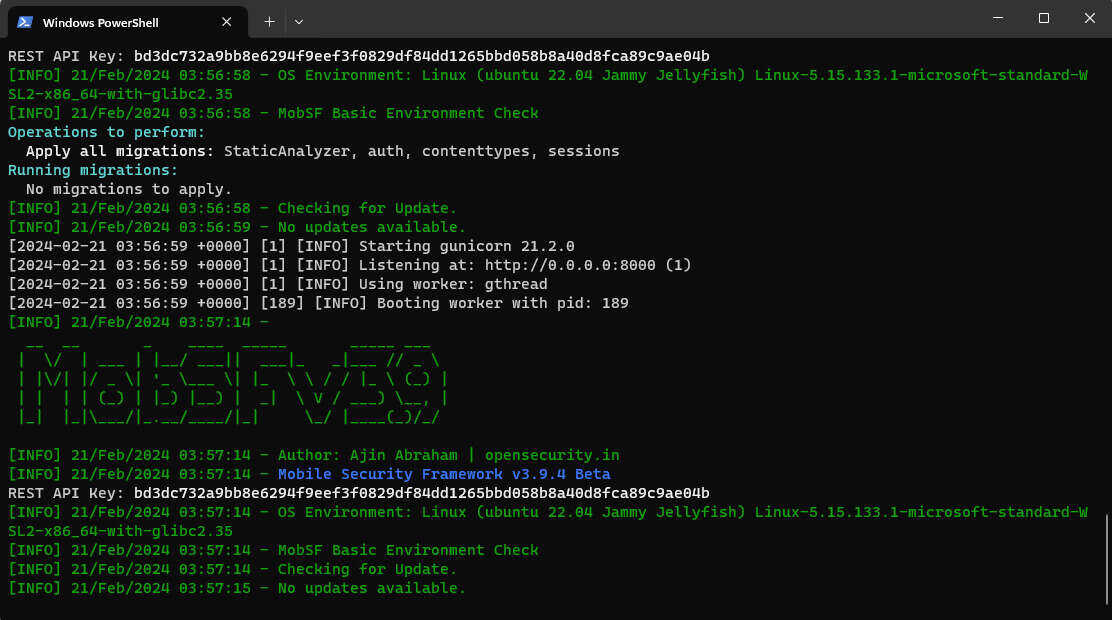
\includegraphics[width=1\textwidth]{images/terminal.jpg}
        \caption{Terminal View}
        \label{fig:example}
    \end{figure}
    \FloatBarrier 
    \item \textbf{Access MobSF Web Interface}: Open your web browser and navigate to \texttt{http://127.0.0.1:8000} (or \texttt{http://localhost:8000}). You should see the MobSF web interface, where you can begin using the framework to analyze mobile applications. It will look like this-
    \begin{figure}[hbt!]
        \centering
        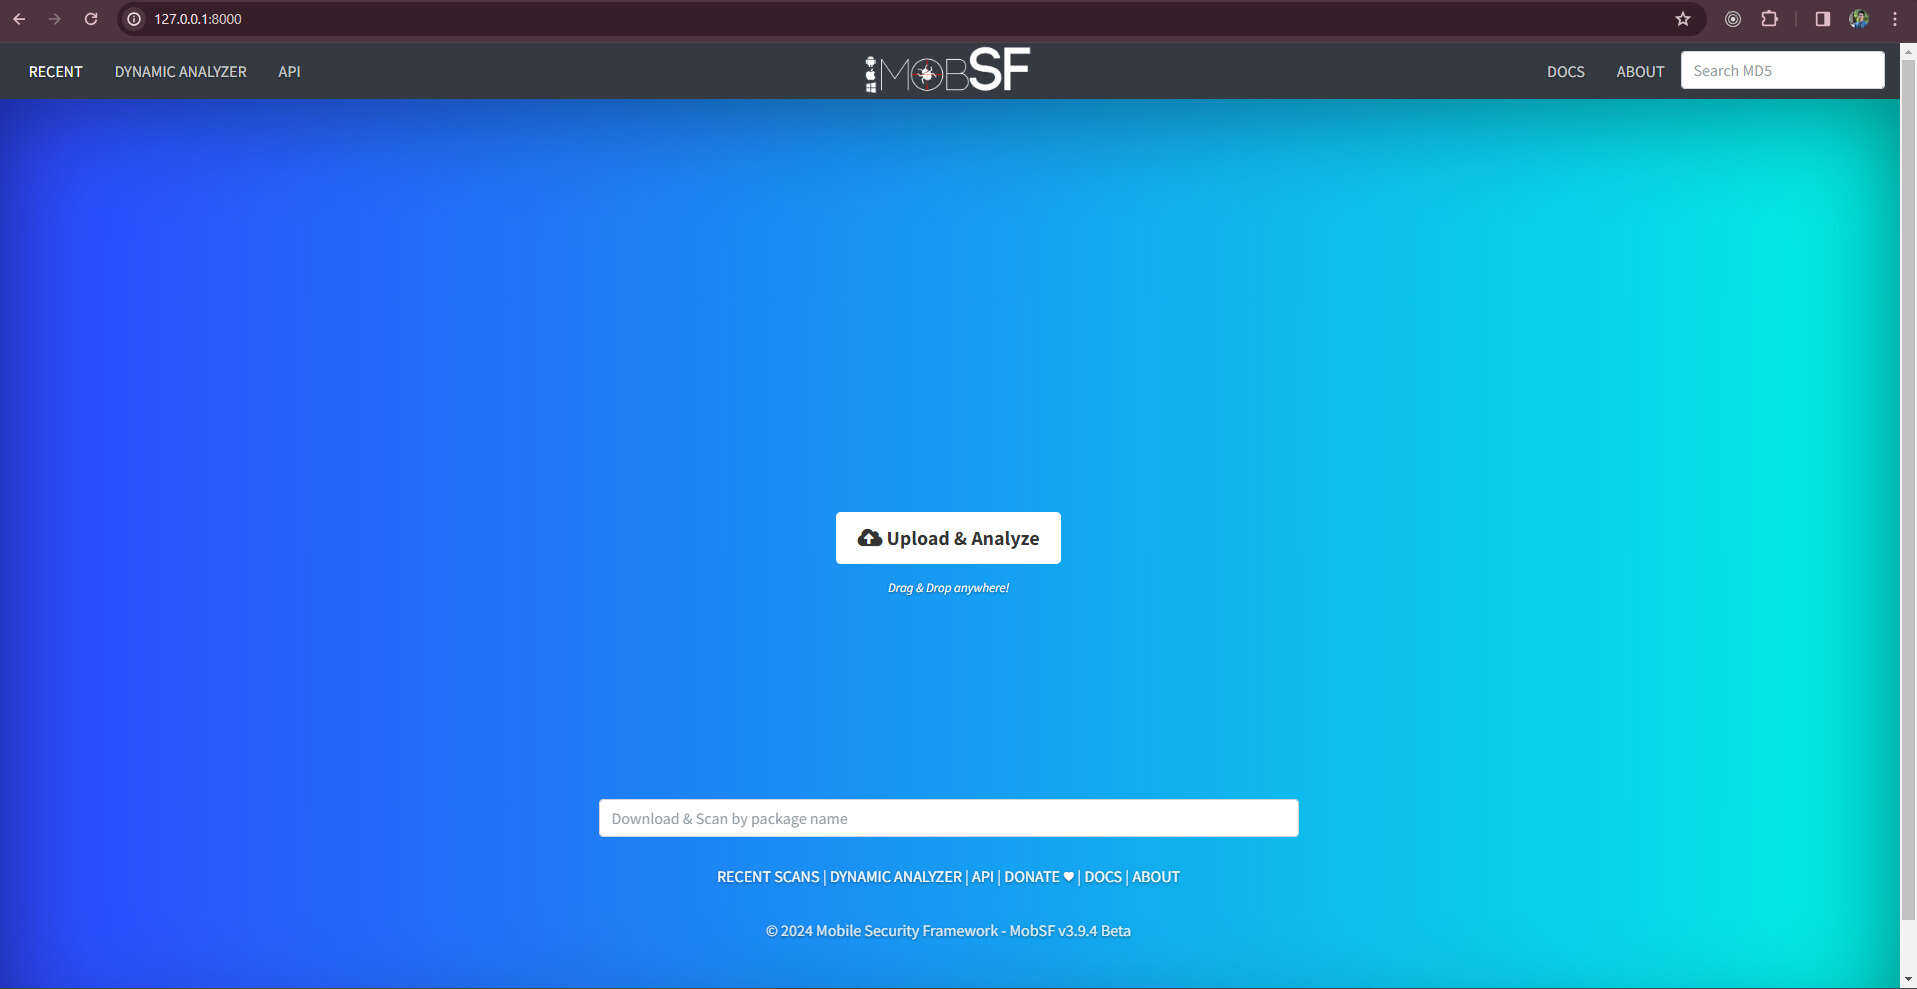
\includegraphics[width=1\textwidth]{images/mobsfwebview.jpg}
        \caption{Web View}
        \label{fig:example}
    \end{figure}
    \FloatBarrier 
    
    \item \textbf{Using MobSF}: You can now use MobSF to upload, analyze, and perform security assessments on mobile applications through the web interface. Follow the on-screen instructions and refer to the MobSF documentation for guidance on using the framework's features.
    
    \item \textbf{Stopping MobSF Container}: To stop the MobSF container, you can press \texttt{Ctrl + C} in the terminal where the container is running. This will gracefully stop the container and exit.

   
\end{enumerate}

That's it! You now have MobSF running using Docker on your system. Docker provides isolation and portability, making it easy to set up and use MobSF in various environments without worrying about dependencies or conflicts.

\chapter{Static Analysis}
We carried out static analysis on an APK Sonali e-wallet. 
\section{Basic Information About The App}
The "Information" feature within MobSF's static analysis procedure offers a significant overview of the mobile application's security and characteristics. It provides important data such as tracker detection count, which reveals possible privacy issues. Additionally, the security score gives an indication of the overall security status of the app. This feature also provides detailed file information, identifying potential risks within the application's components. Furthermore, it offers a thorough summary of the app, covering metadata, permissions, and intent filters, assisting in comprehending its functionality and potential interaction paths. If it is in the playsstore, it also provides a detailed analysis of the playstore information.

\begin{figure}[hbt!]
        \centering
        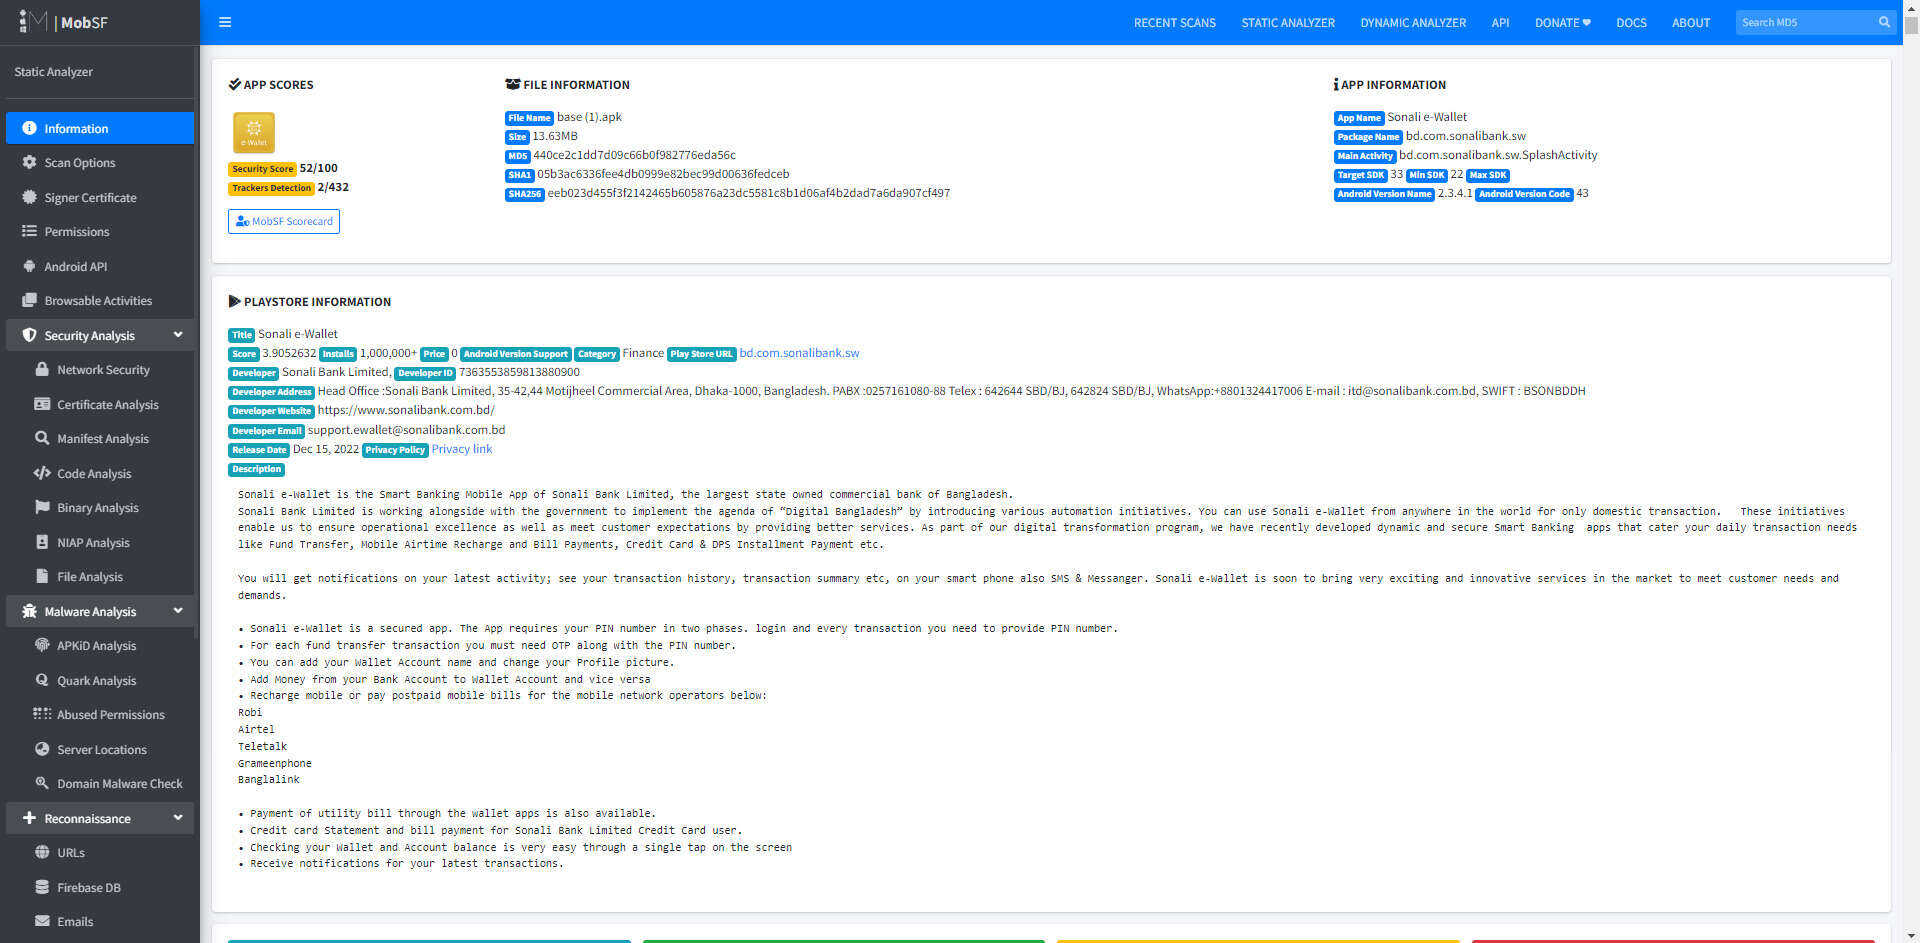
\includegraphics[width=1\textwidth]{images/information.jpg}
        \caption{Basic Information}
        \label{fig:example}
\end{figure}
\FloatBarrier 

\section{Scan Options} 
MobSF's "Scan Options" grant users dynamic control. "Rescan" updates security assessments based on new data or modifications. "Manage Suppressions" aids in handling false positives or ignored findings. "Start Dynamic Analysis" initiates runtime assessment, revealing behavioral vulnerabilities.  Users can also download/view source code and inspect AndroidManifest.xml. 
\begin{figure}[hbt!]
        \centering
        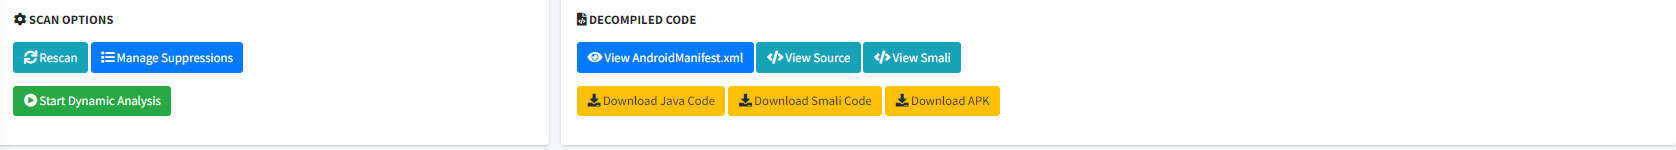
\includegraphics[width=1\textwidth]{images/scan.jpg}
        \caption{Scan Options}
        \label{fig:example}
\end{figure}

\section{Signer's Certificate}
One important element in MobSF that provides information about the legitimacy and dependability of the APK is the "Signer Certificate" function. By providing facts about the signer certificate and the digital signature that was used to confirm the provenance of the app, \newline 
This feature guarantees that the application has not been tampered with or compromised. Users and developers are further reassured by this information that the program originates from a reliable source and hasn't undergone any unauthorized modifications. We can find information like hashing algorithm, public key algorithm, issuer etc in this section. 

\begin{figure}[hbt!]
        \centering
        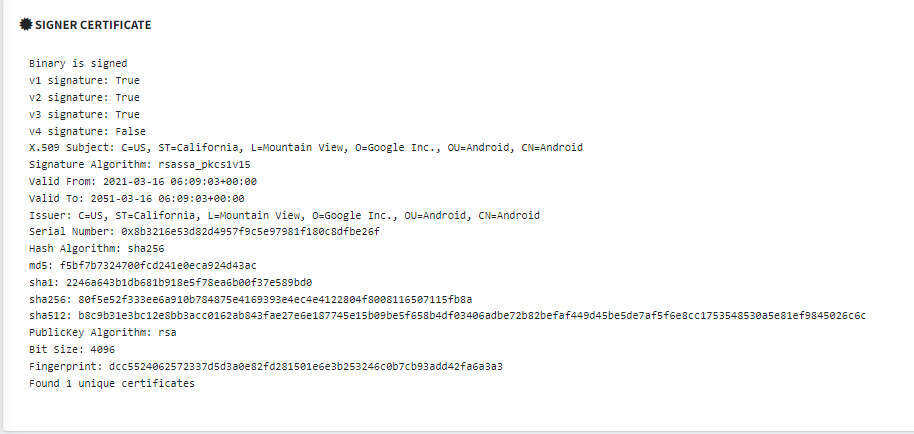
\includegraphics[width=1\textwidth]{images/signer's certificate.jpg}
        \caption{Signer's Certificate}
        \label{fig:example}
\end{figure}

\section{Permissions}
MobSF's "Application Permissions" function provides a detailed analysis of the permissions that the app requests, providing insight into how it uses device resources. For example, "android.permission.ACCESS COARSE LOCATION" or "android.permission.ACCESS NETWORK STATE" is detailed, providing information on whether
it falls under categories like "normal" or "dangerous."  Additionally, the functionality makes it apparent to users how much access each permission entails, providing a clear picture of the applications capabilities.  
By clicking on "Show Files" , users can see which files require this permission and the description section allows a fluent understanding of what the permission encompasses. A point to be noted here is that not all entries that are labelled "dangerous" is actually isn't, it depends on the context whether it is malicious or not.

\begin{figure}[hbt!]
        \centering
        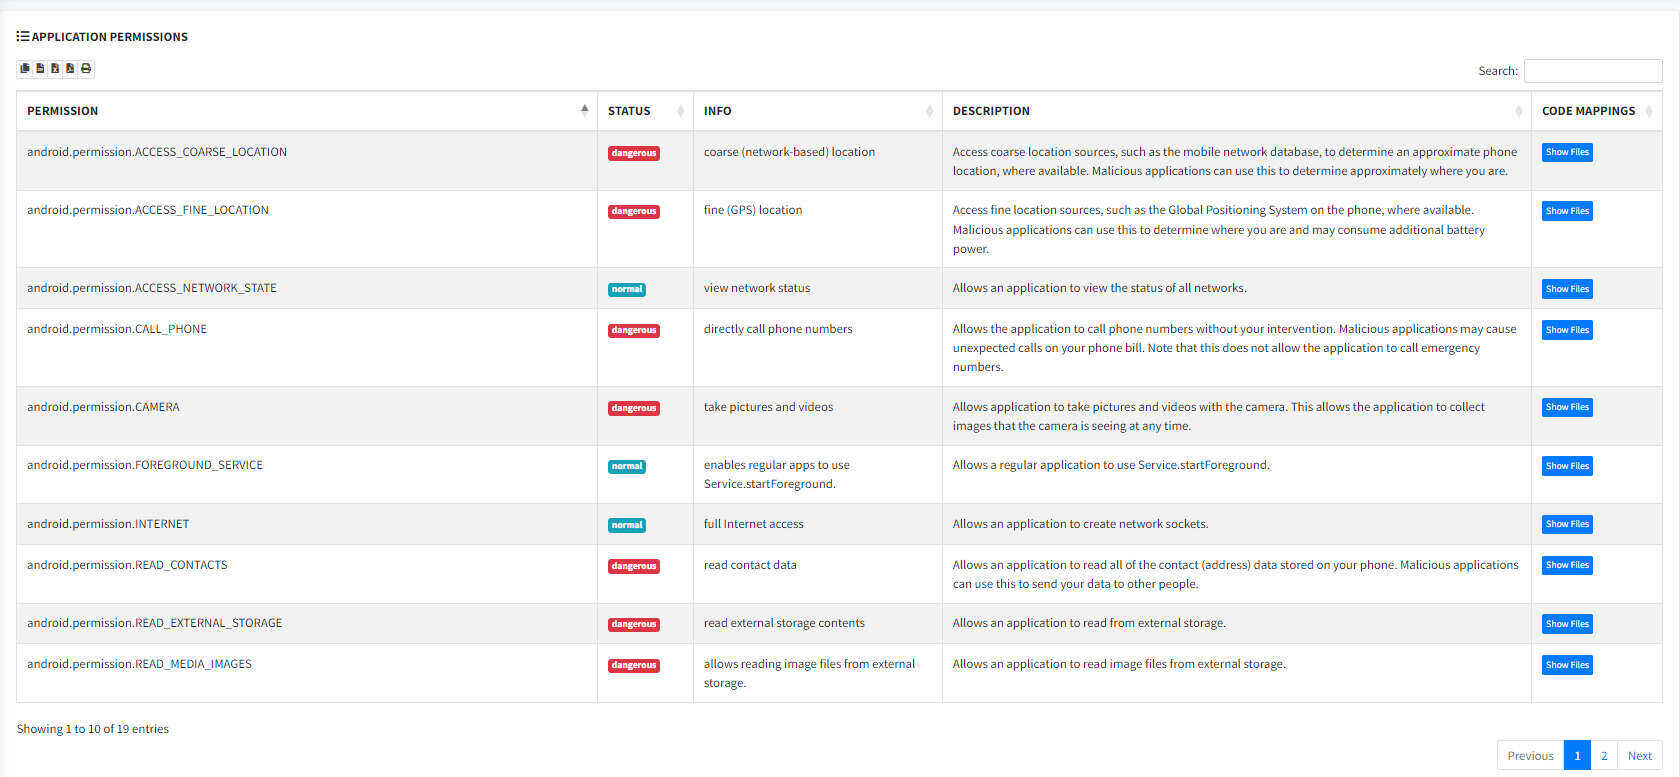
\includegraphics[width=1\textwidth]{images/permisssions.jpg}
        \caption{Application Permission}
        \label{fig:example}
\end{figure}

\FloatBarrier

\section{Android API}

The "Android API" functionality in MobSF provides a concise overview of the mobile app's interaction with the Android API. Presented in an easy-to-read table format, it comprises "API" and "Files" columns. The "API" column lists utilized Android functions, while the "Files" column identifies code files employing each API. This breakdown aids developers in understanding app functionalities, dependencies, and potential security risks, facilitating a deeper comprehension of the app's behavior.

\begin{figure}[hbt!]
        \centering
        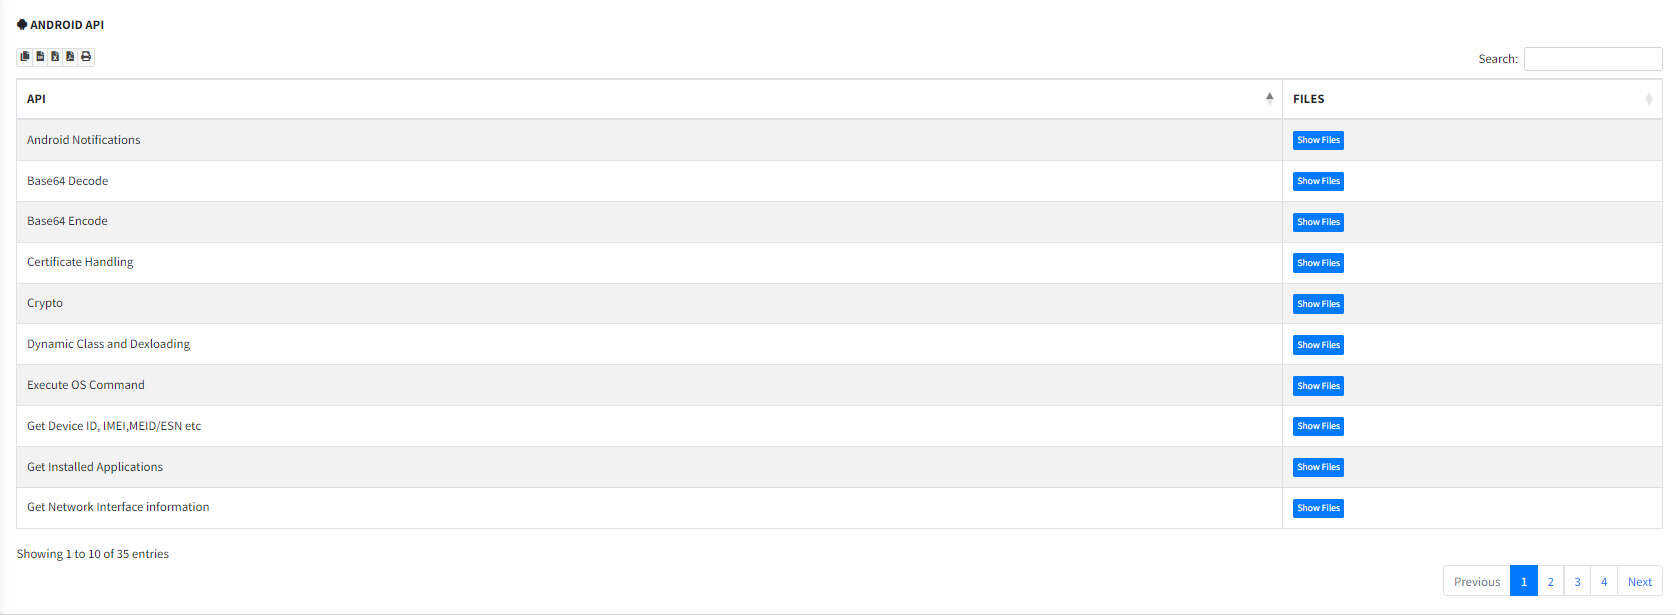
\includegraphics[width=1\textwidth]{images/androidapi.jpg}
        \caption{Android API section}
        \label{fig:example}
\end{figure}

\FloatBarrier

\section{Browsable Activities}
The "Browsable Activities" section in MobSF offers a detailed overview of a mobile app's activities designated as "browsable." which are all the activities that can be browsed by a particular scheme. These activities serve as entry points accessible by other apps or components. MobSF identifies and highlights these activities, providing crucial insights into accessible app sections from external sources. This feature is vital for pinpointing security vulnerabilities, as certain browsable activities may inadvertently expose sensitive functionalities to unauthorized entities. By detecting such risks, developers can proactively mitigate security concerns, ensuring the protection of user data and bolstering the app's overall security posture within a comprehensive security assessment framework.

\begin{figure}[hbt!]
        \centering
        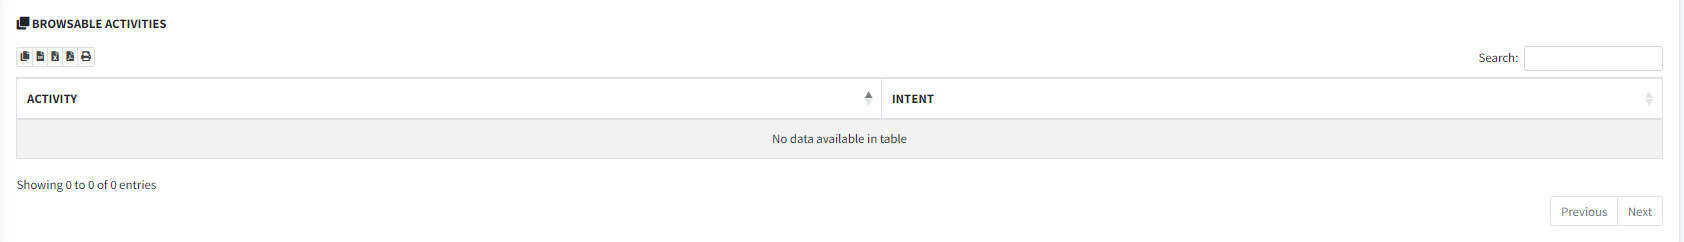
\includegraphics[width=1\textwidth]{images/browsable.jpg}
        \caption{Browsable Activities}
        \label{fig:example}
\end{figure}
\FloatBarrier

\section{Security Analysis}
\subsection{Network Security}
MobSF's "Network Security" function is crucial for assessing network-related aspects of mobile apps. It organizes findings into "High," "Warning," and "Info" categories, facilitating prioritization. Counts for each category offer insight into issue severity and prevalence. A detailed table presents key details including "Scope," "Severity," and "Description," aiding comprehension of network security threats by outlining context, impact, and explanation for developers and security experts.
\begin{figure}[hbt!]
        \centering
        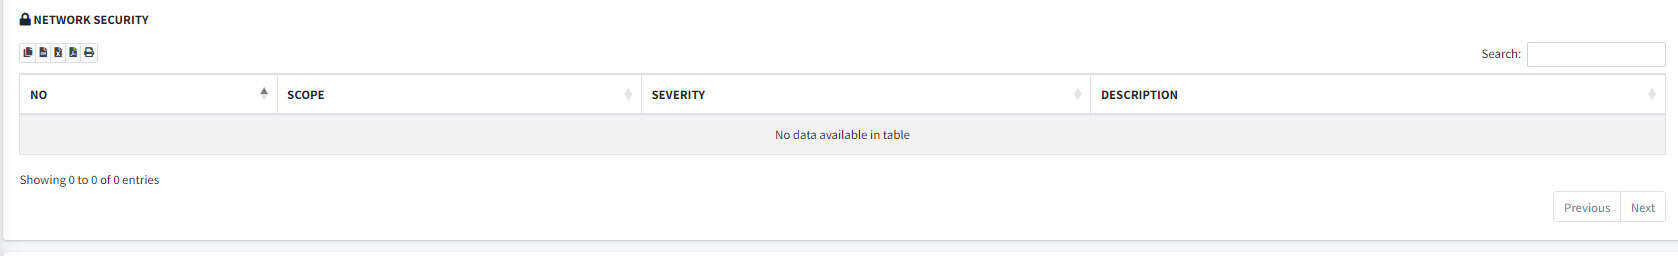
\includegraphics[width=1\textwidth]{images/networksecu.jpg}
        \caption{Network Security}
        \label{fig:example}
\end{figure}
\FloatBarrier

\subsection{Certificate Analysis}
The "Certificate Analysis" functionality in MobSF is a crucial aspect that assesses the security of certificates utilized by a mobile app. It categorizes findings into "High," "Warning," "Info," and "Secure," indicating the severity of certificate-related issues. Counts for each category offer a quick overview of prevalence and severity. Furthermore, a detailed table presents key details including "Title," "Severity," and "Description," aiding understanding of certificate vulnerabilities for developers and security professionals.
\begin{figure}[hbt!]
    \centering
    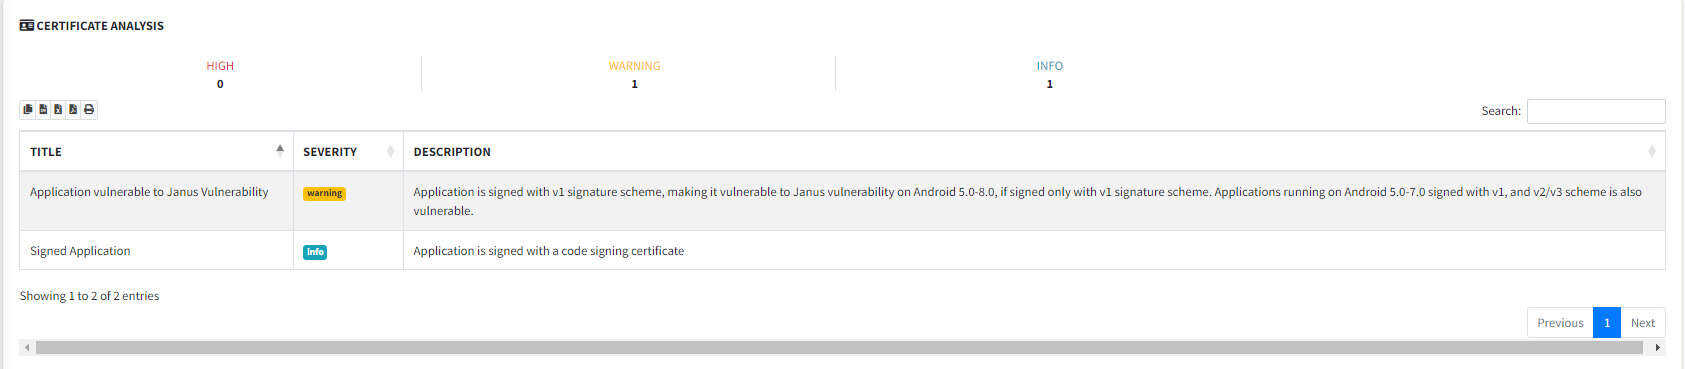
\includegraphics[width=1\textwidth]{images/certificate_analysis.jpg}
    \caption{Certificate Analysis}
    \label{fig:example}
\end{figure}
\FloatBarrier

\subsection{Manifest Analysis}
The "Manifest Analysis" function in MobSF is essential for assessing the security of an app's manifest file, which contains vital information about its components and permissions. It sorts findings into categories like "High," "Warning," "Info," and "Suppressed," clarifying the severity of manifest-related issues. Counts for each category offer a quick summary of severity. A comprehensive table is also provided, including important columns such as "Issue," "Severity," "Description," and "Options," to help users comprehend and efficiently resolve vulnerabilities connected to manifests. The "Options" column can be used to suppress the rules for that particular manifest. Clicking "Suppress" on the pop-up window, the users can suppress that rule.
\begin{figure}[hbt!]
        \centering
        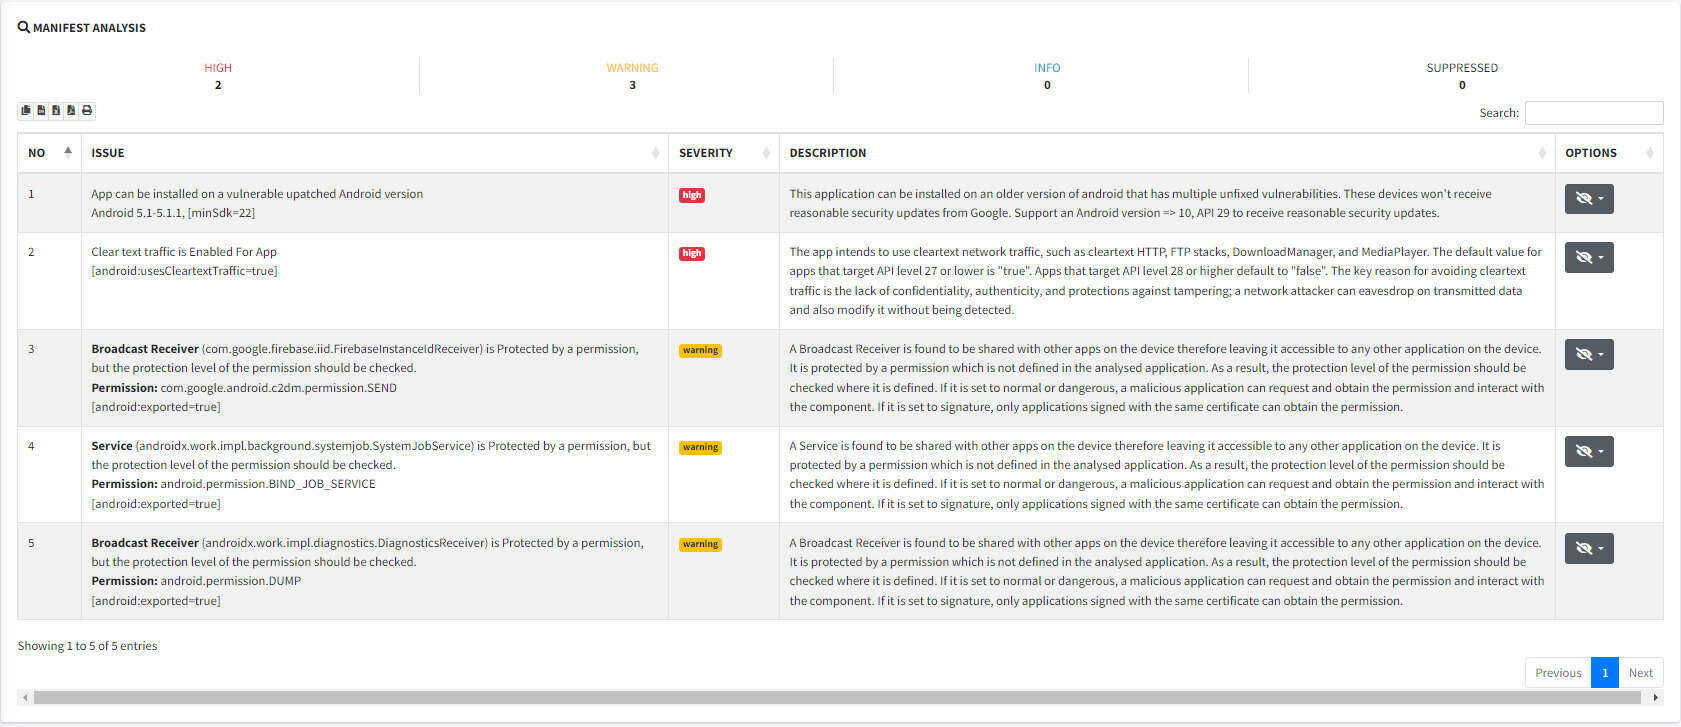
\includegraphics[width=1\textwidth]{images/manifest.jpg}
        \caption{Manifest Analysis}
        \label{fig:example}
\end{figure}
\FloatBarrier
\begin{figure}[hbt!]
    \centering
    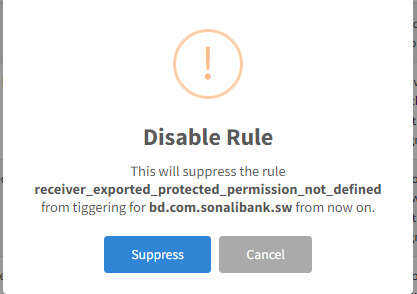
\includegraphics[width=0.5\textwidth]{images/supressrule.jpg}
    \caption{Supression Rule}
    \label{fig:example}
\end{figure}
\FloatBarrier

\subsection{Code Analysis}

The "Code Analysis" feature in MobSF is integral for evaluating the security of an application's underlying codebase. This is where MobSF has performed analysis on all of the decompiled java files.  It categorizes findings into distinct levels, including "High," "Warning," "Info," "Secure," and "Suppressed," based on different standards like CW. OWASP etc. facilitating users' understanding of the seriousness and nature of code-related issues. Providing counts for each category offers a concise representation of the prevalence and severity of these concerns.\newline
This feature presents a comprehensive table with key columns such as "Issue," "Severity," "Standards," "Files," and "Options." In the "Issue" column, it succinctly outlines the specific code-related problem detected, offering clarity on the identified issues. The "Severity" column indicates the potential impact of these issues on the application's security, allowing users to prioritize remediation efforts effectively.
\newline
Moreover, the "Standards" column may highlight relevant security standards or best practices that the detected issues violate, guiding developers towards compliance with industry norms. The "Files" column points to specific code files associated with each concern, enabling targeted analysis and resolution.
\newline
Lastly, the "Options" column provides users with choices to suppress certain issues if necessary, offering flexibility in managing and addressing identified vulnerabilities. This multifaceted approach empowers users to comprehensively assess, understand, and mitigate code-related security risks within their applications\newline
\begin{figure}[hbt!]
    \centering
    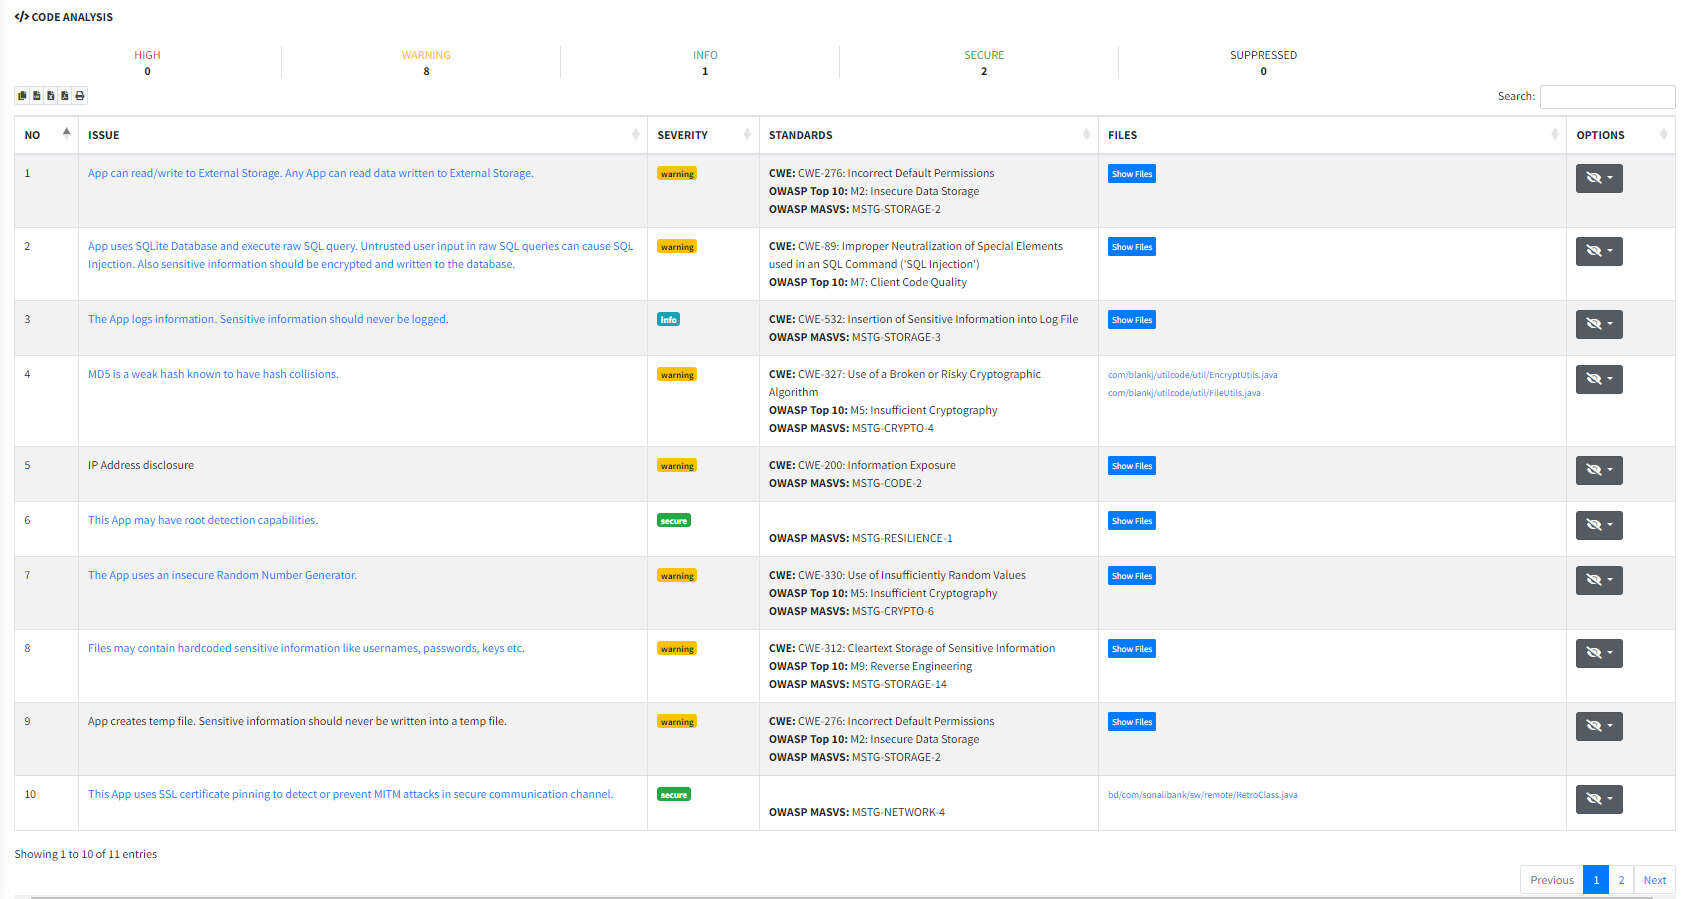
\includegraphics[width=1\textwidth]{images/codeanalysis.jpg}
    \caption{Code Analysis}
    \label{fig:example}
\end{figure}
\FloatBarrier

\subsection{Binary Analysis}
Shared library binary analysis is important if your code has native files, i.e is any of the files isn't compiled properly. MobSF's "Binary Analysis" assesses app security through compiled binary files. It provides a detailed table with the following key attributes:
\begin{itemize}
    \item \textbf{NX}: Marks a memory page non-executable, preventing execution of injected shellcode. Either True or False.
    \item \textbf{Stack Canary}: Detects and prevents exploits from overwriting return addresses. Applicable with -fstack-protector-all option. Not applicable for Dart/Flutter libraries unless Dart FFI is used. Either True or False.
    \item \textbf{RELRO}: Ensures the Global Offset Table (GOT) cannot be overwritten in vulnerable ELF binaries. "Full" indicates the entire GOT (.got and .got.plt both) is read-only. Either Full or Not Applicable.
    \item \textbf{RPATH}: Represents the runtime path (RPATH) of the binary, indicating locations where the binary searches for shared libraries.
    \item \textbf{RUNPATH}: Specifies library search paths with different loading semantics. Similar to RPATH.
    \item \textbf{FORTIFY}: Indicates presence of buffer overflow protection mechanism. Either True or False depending on presence.
    \item \textbf{SYMBOLS STRIPPED}: Denotes if binary's symbols have been stripped, making reverse engineering more difficult. Either True or False depending on presence.
\end{itemize}

\begin{figure}[hbt!]
    \centering
    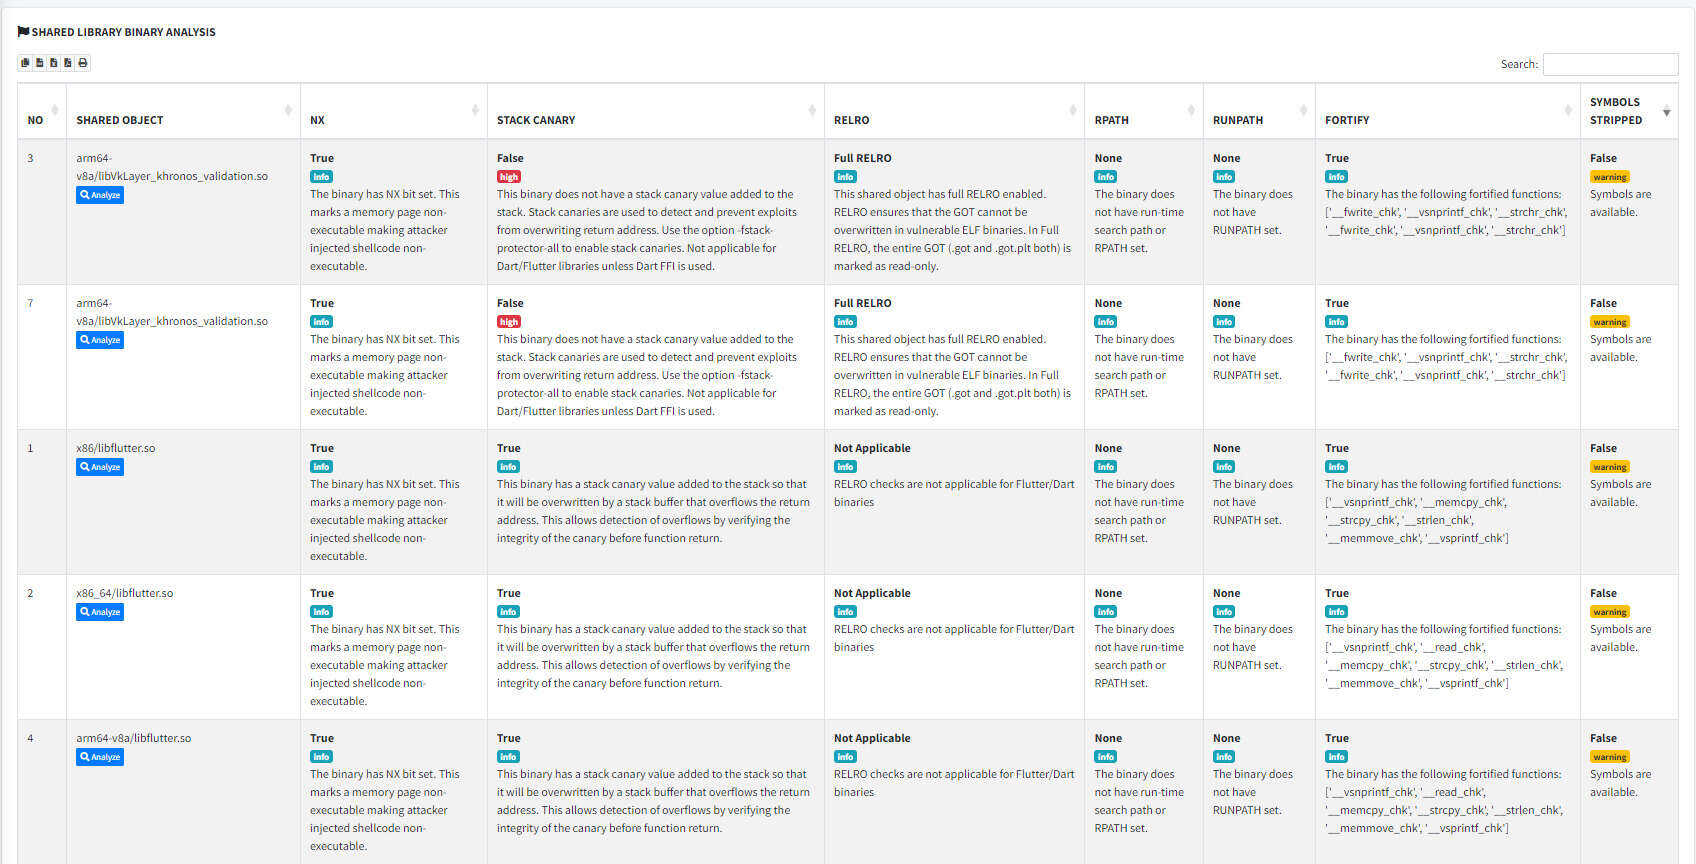
\includegraphics[width=1\textwidth]{images/binaryanalysis.jpg}
    \caption{Binary Analysis}
    \label{fig:example}
\end{figure}
\FloatBarrier

\subsection{NIAP Analysis}
The National Information Assurance Partnership (NIAP) is a United States government initiative that oversees the evaluation and certification of commercial off-the-shelf (COTS) information technology (IT) products for conformance to the international Common Criteria security evaluation standards. his functionality presents users with a detailed table comprising four essential columns: "Identifier," "Requirement," "Feature," and "Description."
The "Identifier" column showcases a unique code associated with each NIAP requirement, aiding users in quickly distinguishing and referencing individual requirements.
In the "Requirement" column, specific security or compliance standards mandated by NIAP are outlined, serving as benchmarks for the evaluation process.
The "Feature" column illuminates the application's characteristics or functionalities that directly align with or fulfill the NIAP requirements. This linkage between requirements and app features facilitates a clear understanding of how the application meets established standards.
Providing further context, the "Description" column offers additional explanations for each NIAP requirement. These descriptions elaborates the significance of adhering to these standards, aiding users in understanding the importance of meeting each criterion for robust security and compliance.

\begin{figure}[hbt!]
    \centering
    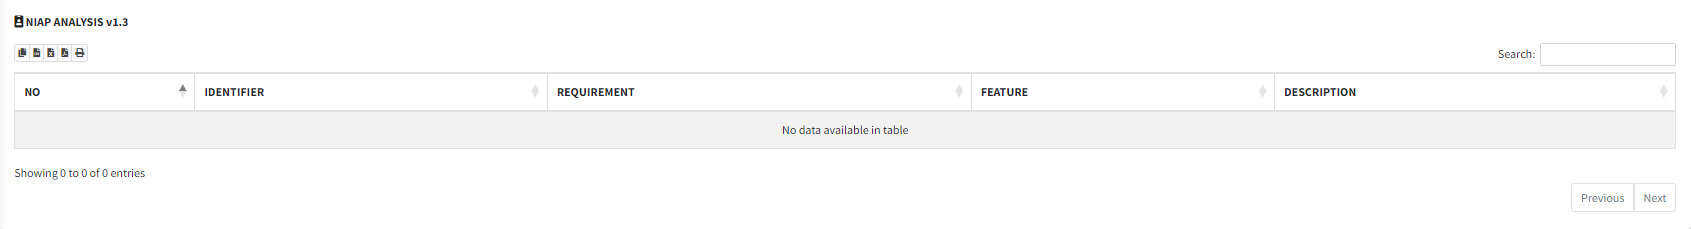
\includegraphics[width=1\textwidth]{images/niap.jpg}
    \caption{NIAP Analysis}
    \label{fig:example}
\end{figure}
\FloatBarrier

\subsection{File Analysis}
This section will actually star out all the the sensitive files that are hardcoded inside the application, for example- if anyone uploads private keys accidentally.
In the "Issue" column, the feature concisely describes specific vulnerabilities, or discrepancies detected within the application's files. These issues may encompass a wide range of potential problems, including security vulnerabilities or deviations from established best practices.\newline
Meanwhile, the "Files" column enumerates the individual files within the application that are associated with each identified issue. This direct correlation between the issue and the implicated files facilitates a clear understanding of where within the application the problem resides, enabling users to address and remediate issues effectively.

\begin{figure}[hbt!]
    \centering
    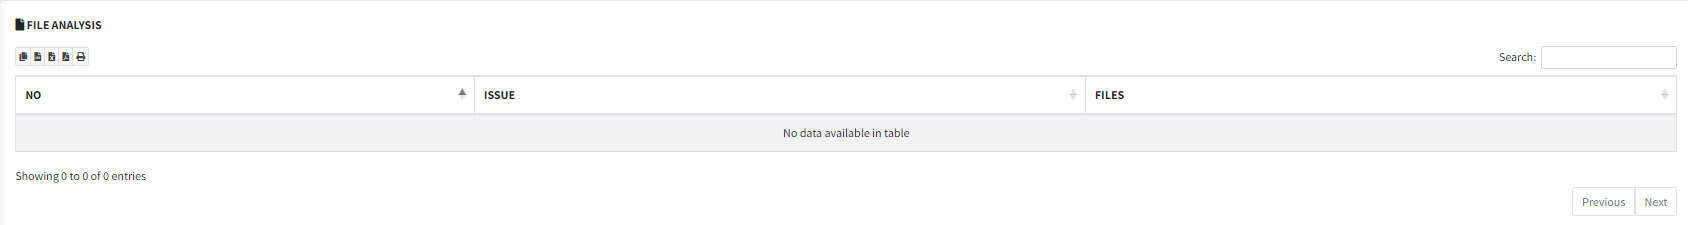
\includegraphics[width=1\textwidth]{images/fileanalysis.jpg}
    \caption{File Analysis}
    \label{fig:example}
\end{figure}
\FloatBarrier


\section{Malware Analysis}
\subsection*{APKiD Analysis}
Apk id analysis apk-id looks into the dex files and
tells us the possible behavioral patterns like the kind of compiler being used if
an obfuscator was used or does the dex file has code that corresponds to a vm detection or anti-debugging checks things like that so it gives you a good idea about the behavior of the application from code perspective. This feature presents a structured table comprising two essential columns: "DEX" and "Detection."
In the "DEX" column, details regarding the Dalvik Executable (DEX) files within the APK are presented. These files contain the executable bytecode that runs on Android devices. The "Detection" column succinctly indicates the detection results, highlighting the presence of compilers, packers, obfuscators, or other notable attributes identified during the analysis process.

\begin{figure}[hbt!]
    \centering
    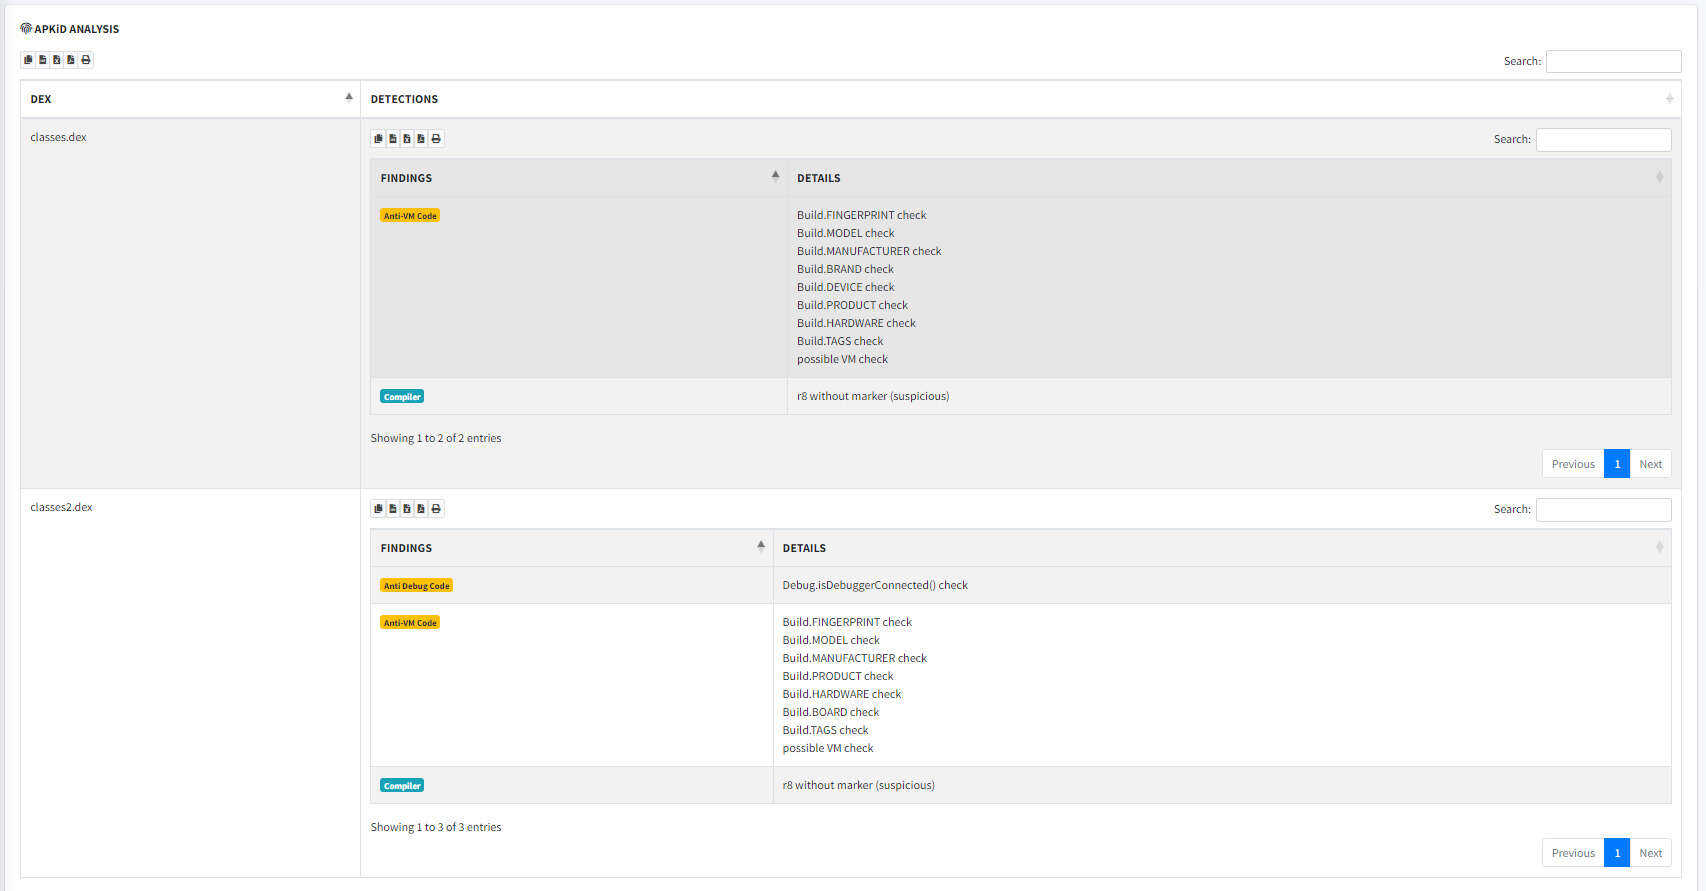
\includegraphics[width=1\textwidth]{images/apkid.jpg}
    \caption{APKiD Analysis}
    \label{fig:example}
\end{figure}
\FloatBarrier

\subsection{Quark Analysis}
Quark-Engine is indeed a powerful Android analysis framework designed to delve into APK and DEX files to uncover potential threats and gather intelligence regarding malicious activities. When integrated into MobSF, Quark-Engine enhances the platform's capabilities by providing advanced analysis features. It consists of two fields "Potential Malicious Behavior" and "Evidence" from which details about the malicious behaviors can be known.  

\begin{figure}[hbt!]
    \centering
    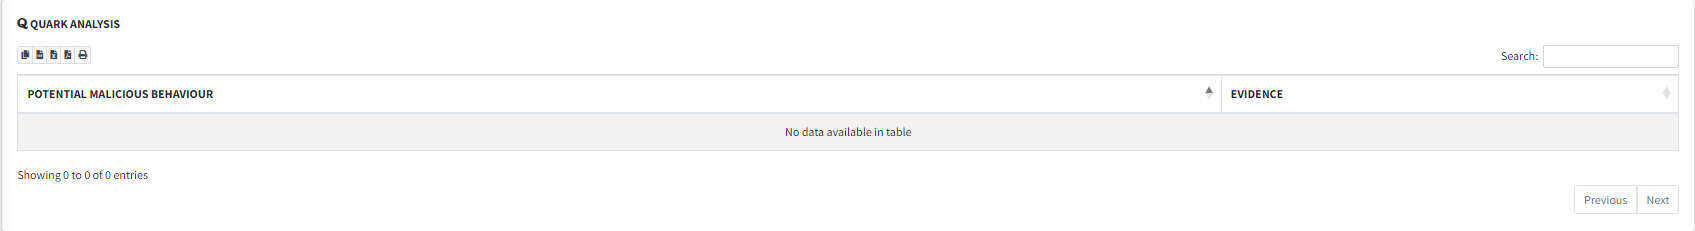
\includegraphics[width=1\textwidth]{images/quark.jpg}
    \caption{Quark Analysis}
    \label{fig:example}
\end{figure}
\FloatBarrier

\subsection{Abused Permissions}
In MobSF, the abused permission section highlights the potential permissions that are widely used by common malware and other common permissions that are used by known malware.\newline
Malware Permissions: Permissions commonly exploited by malware for malicious activities.\newline
Other Common Permissions: Permissions commonly requested by legitimate apps but could pose security or privacy risks if misused.\newline
This categorization helps users quickly identify potential security concerns associated with permissions requested by Android applications.
\begin{figure}[hbt!]
    \centering
    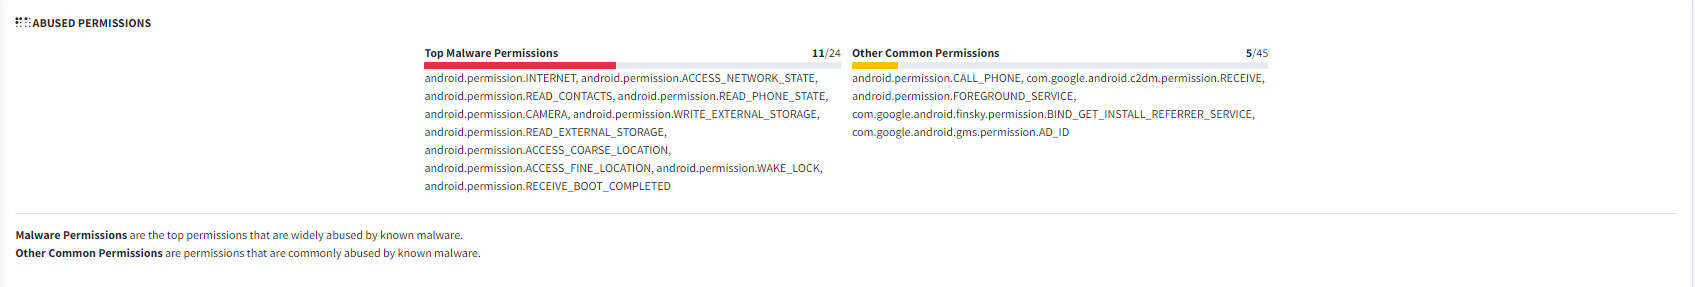
\includegraphics[width=1\textwidth]{images/abusedpermissions.jpg}
    \caption{Abused Permissions}
        \label{fig:example}
\end{figure}
\FloatBarrier

\subsection*{Server Locations}
Server Locations denote where the servers used in this app resides. The domain sanction provides OFAC sanctioned list of countries with which this app may communicate.
\begin{figure}[hbt!]
    \centering
    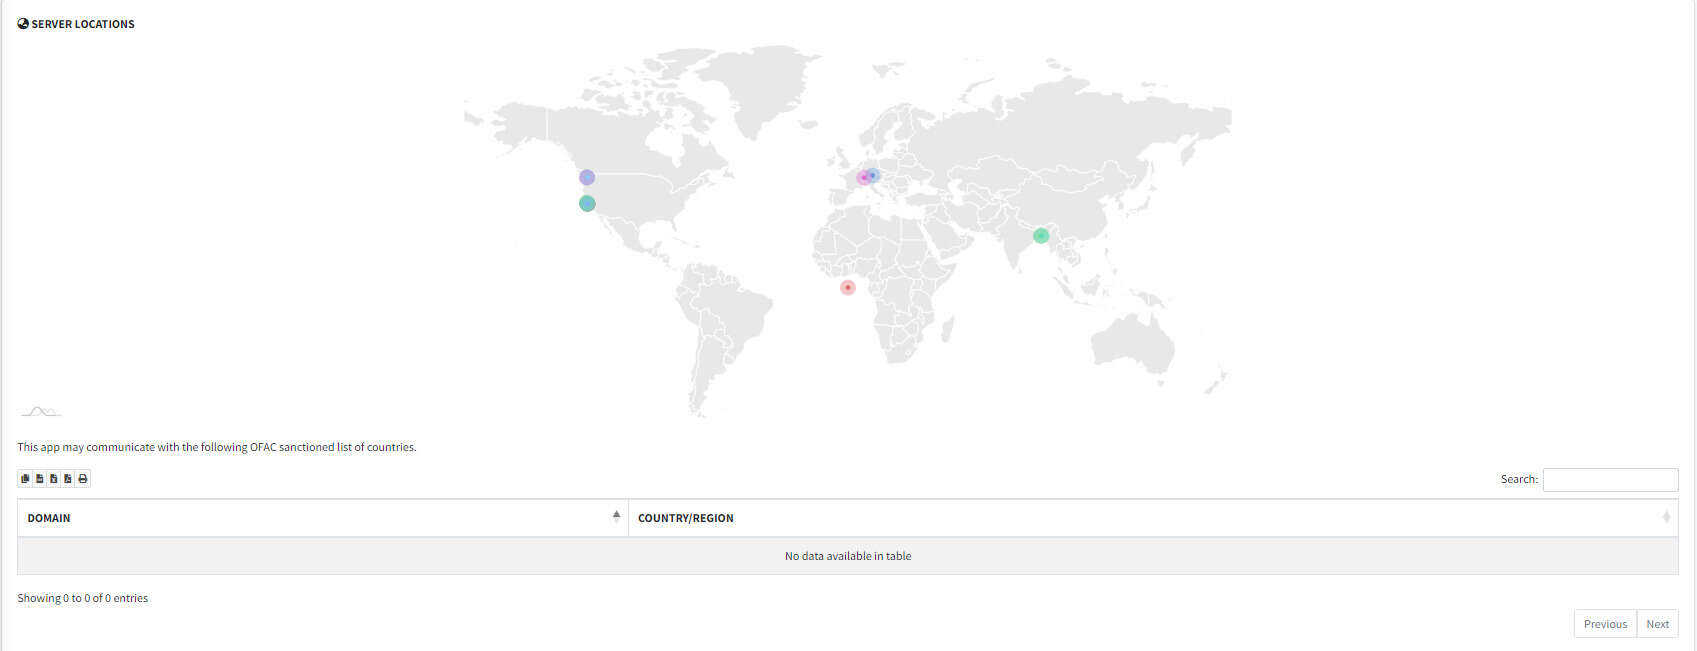
\includegraphics[width=1\textwidth]{images/serverlocations.jpg}
    \caption{Server Locations}
    \label{fig:example}
\end{figure}
\FloatBarrier

\subsection{Domain Malware Check}
The Domain Malware Check feature essentially extracts all domains from the binary and cross-references them against a database of known malicious or suspicious domains and IPs. This database contains entries of non-malware-related IPs and domains. Each domain found within the binary is compared against this database to determine if it is present, thereby assessing its status as either good or bad. \newline
Additionally, geolocation data is retrieved for all identified domains within the application. This information can then be visualized, potentially on a platform like Google Maps, to provide insight into the geographical locations associated with the IP addresses. \newline
Overall, this feature offers a comprehensive assessment of the domains within the binary, allowing users to identify potential security threats and gain insight into the geographical distribution of the associated IP addresses.
\begin{figure}[hbt!]
    \centering
    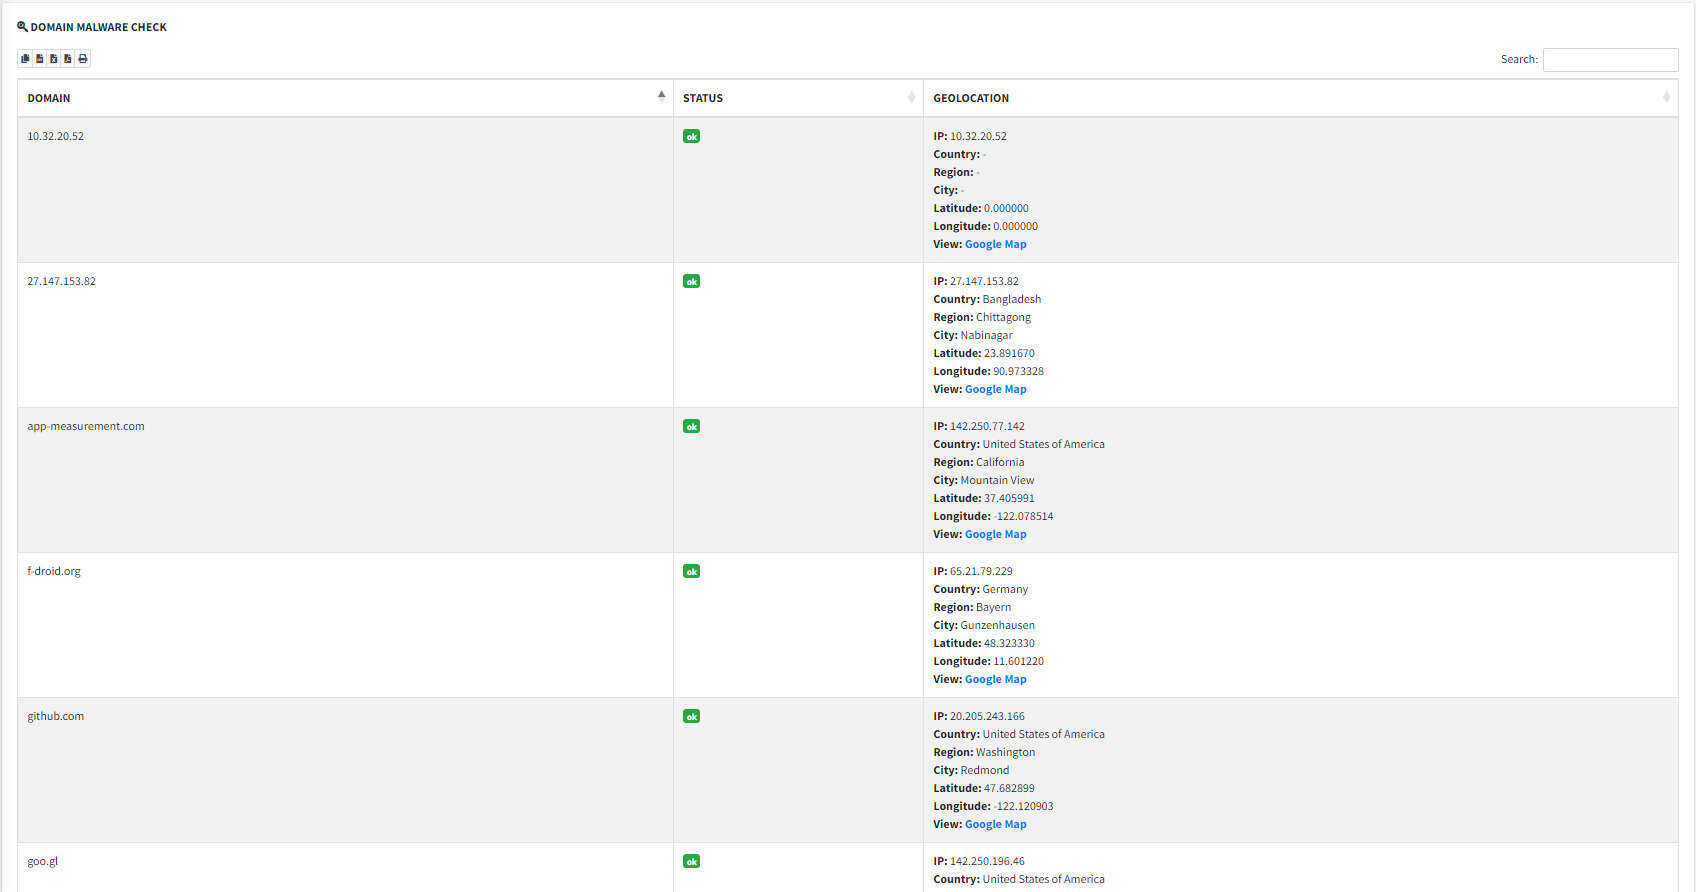
\includegraphics[width=1\textwidth]{images/domain_malware_check.jpg}
    \caption{Domain Malware Check}
    \label{fig:example}
\end{figure}
\FloatBarrier

\section{Reconnaissance}
\subsection{URLs}
MobSF will list all URLs extracted from various parts of the application's source code, including manifest files, Java code, native code, resources, JavaScript, and HTML files. 
\begin{figure}[hbt!]
    \centering
    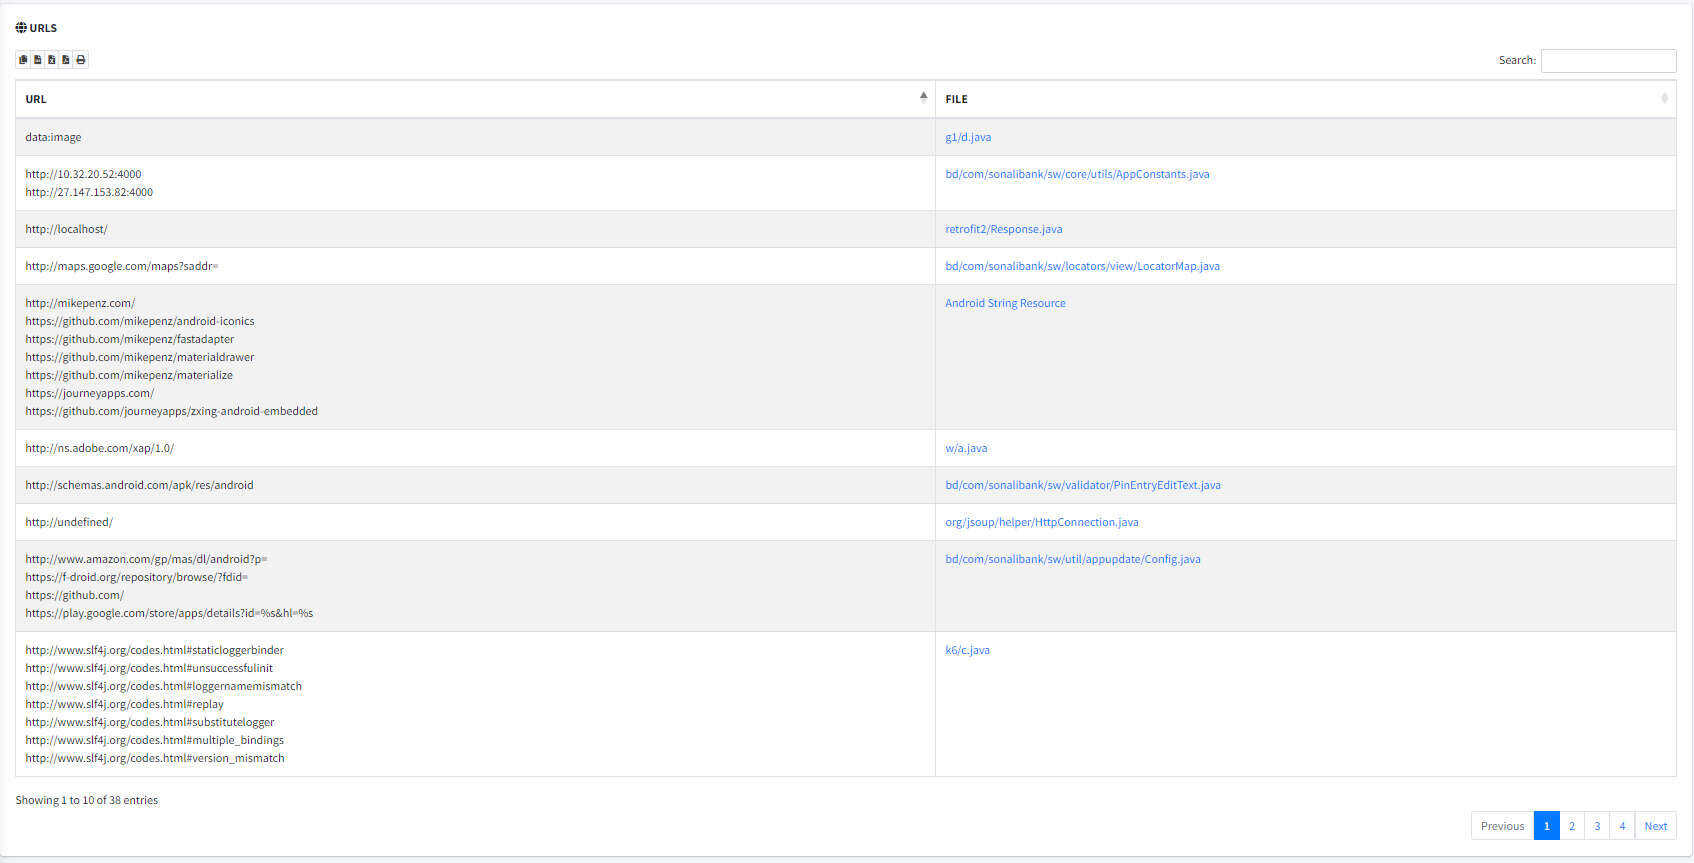
\includegraphics[width=1\linewidth]{images/url.jpg}
    \caption{URL}
    \label{fig:example}
\end{figure}
\FloatBarrier

\subsection{Firebase DB}
MobSF will also extract all the firebase database url from the app and it also performs an additional check to see if the database is exposed to the internet
\begin{figure}[hbt!]
    \centering
    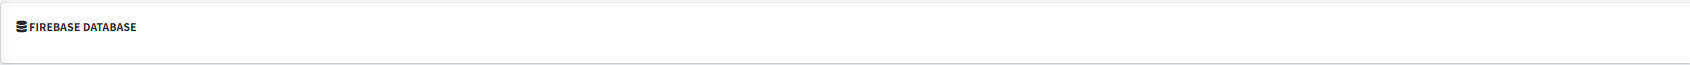
\includegraphics[width=1\linewidth]{images/firebase.jpg}
    \caption{Firebase DB}
    \label{fig:example}
\end{figure}
\FloatBarrier

\subsection{Emails}
MobSF shows all the email ids used in the code along with their corresponding file location in this section.
\begin{figure}[hbt!]
    \centering
    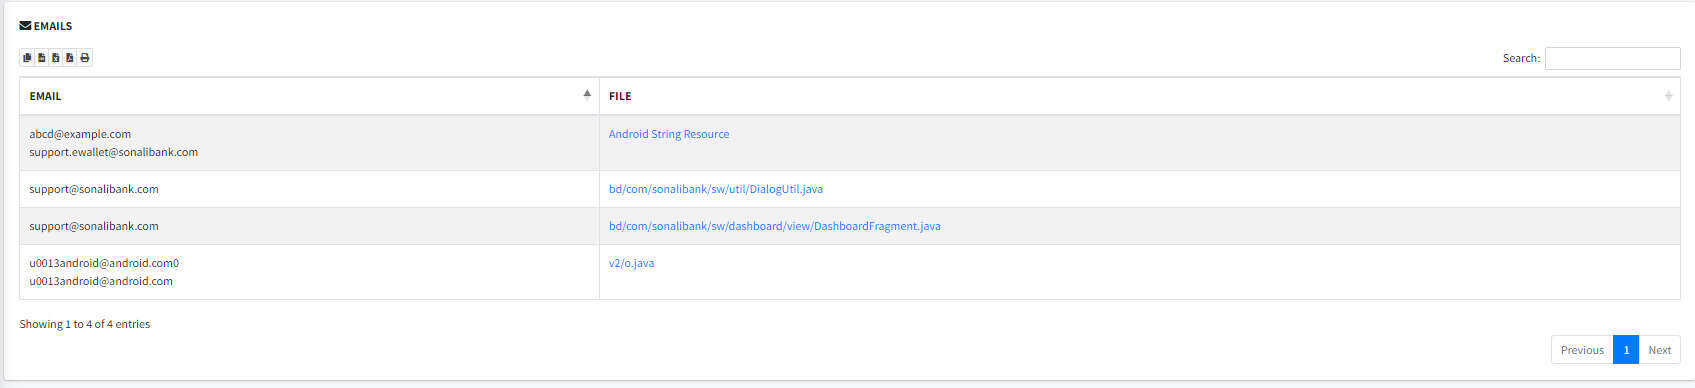
\includegraphics[width=1\linewidth]{images/email.jpg}
    \caption{Emails}
    \label{fig:example}
\end{figure}
\FloatBarrier

\subsection{Possible Hardcoded Secrets}
In this section, MobSF highlights possible hardcoded secrets such as Google API keys, Map API keys, and crash reporting API keys etc. found within the application's source code. By identifying these hardcoded secrets, MobSF helps developers detect and address potential security vulnerabilities related to sensitive information exposure.section.
\begin{figure}[hbt!]
    \centering
    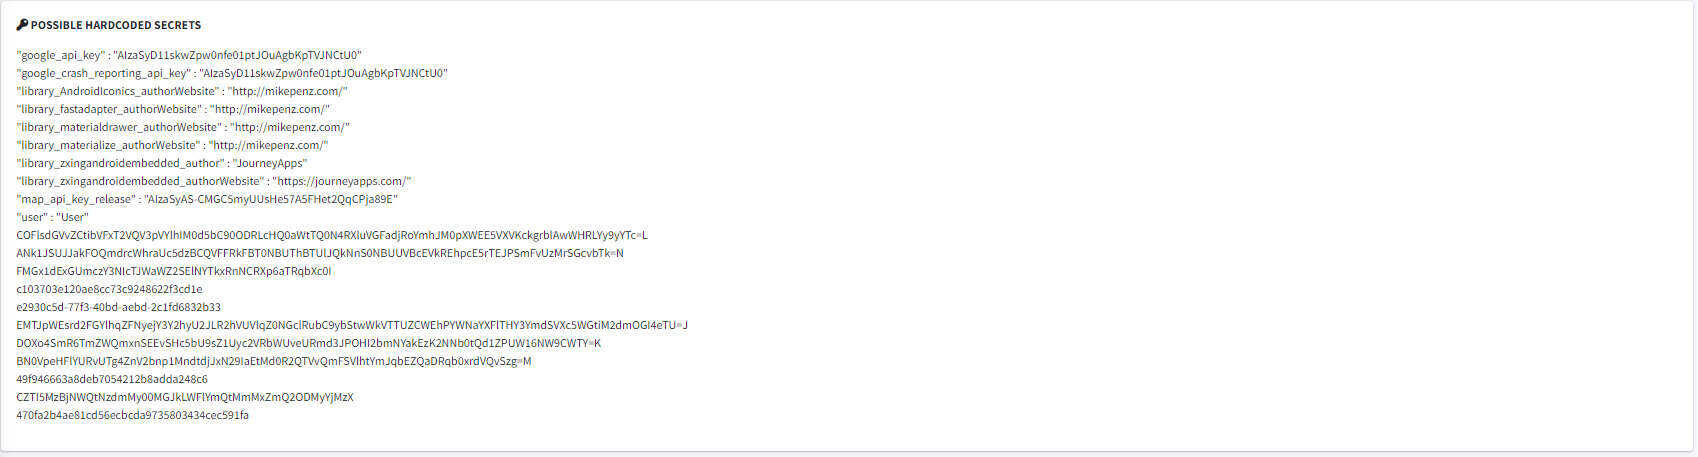
\includegraphics[width=1\linewidth]{images/psbl_secrets.jpg}
    \caption{Possible Hardcoded Secrets}
    \label{fig:example}
\end{figure}
\FloatBarrier

\subsection{Strings}
In this section, MobSF presents all the hardcoded strings extracted from the binary, including those from string resources. This includes sensitive information such as API keys and other secrets that may have been hardcoded into the application.
11:49
dumbed and shown over heresection.
\begin{figure}[hbt!]
    \centering
    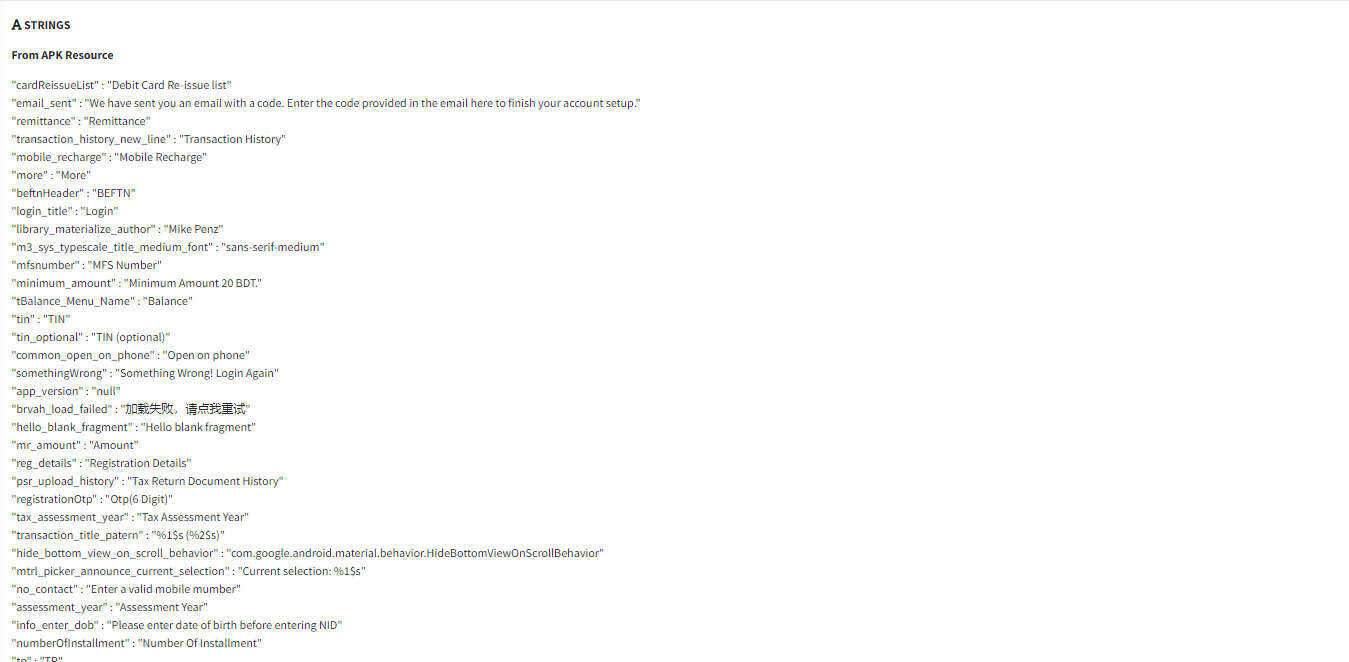
\includegraphics[width=1\linewidth]{images/strings.jpg}
    \caption{Strings}
    \label{fig:example}
\end{figure}
\FloatBarrier

\chapter{Dynamic Analysis}
\section{Setup for Dynamic Analysis}
MobSF supports certain rooted Android VMs/emulators created with: Genymotion, Genymotion Cloud VM, Android Studio Emulator, Corellium .MobSF also supports jailbroken iOS virtual devices created with Corellium. Detailed steup for each processes can be found in this link - \newline \href{https://mobsf.github.io/docs/#/dynamic_analyzer}{https://mobsf.github.io/docs/\#/dynamic\_analyzer}
\section{Start Dynamic Analysis}
Do the static analysis first. Then click on the Start Dynamic Analysis button. You can find it on "Scan Options" tab. After some time this screen will appear -

% will add image

\begin{figure}[hbt!]
    \centering
    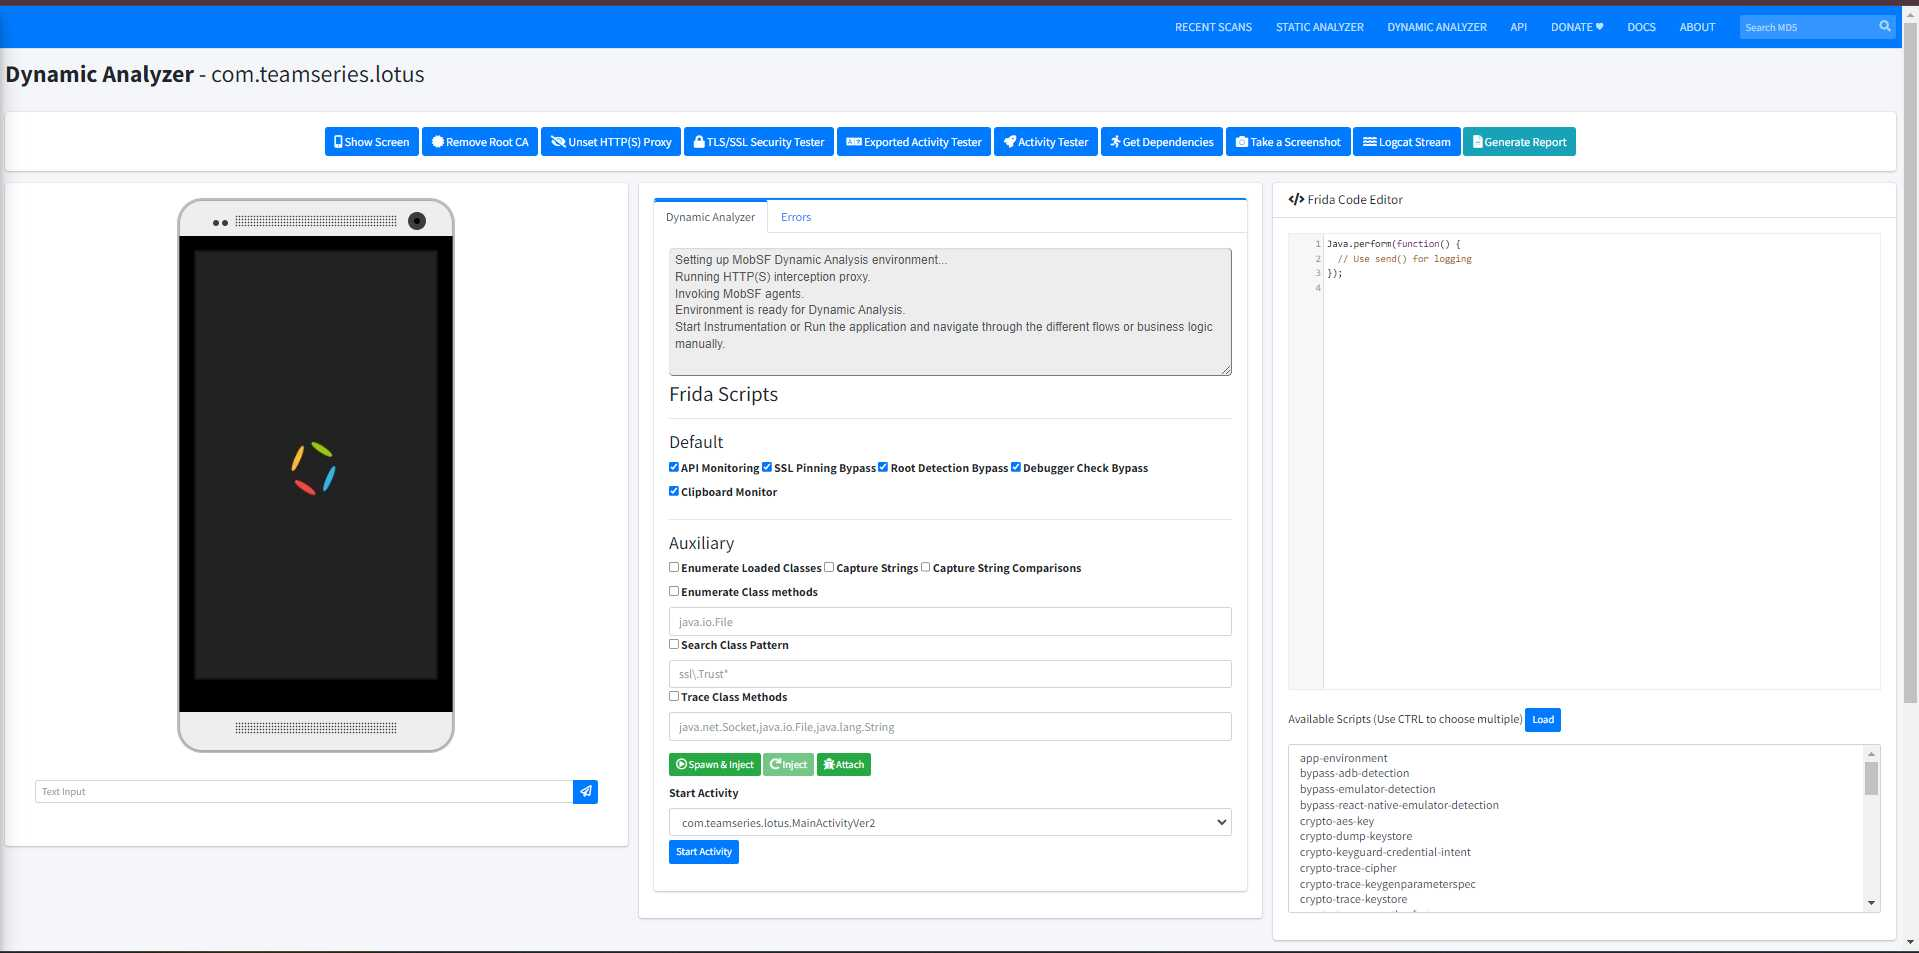
\includegraphics[width=1\linewidth]{Dynamic Analyzer/dynamic_screen.jpg}
    \caption{Dynamic Analysis}
    \label{fig:example}
\end{figure}
\FloatBarrier


Inside the dynamic analyzer there is this screen with the options-

\begin{figure}[hbt!]
    \centering
    
\includegraphics[width=1\linewidth]{Dynamic Analyzer/options.jpg}
    \caption{Options}
    \label{fig:example}
\end{figure}
\FloatBarrier

\subsection{Show Screen}
There is a show screen option to view current screen of the emulator.
\begin{figure}[hbt!]
    \centering
    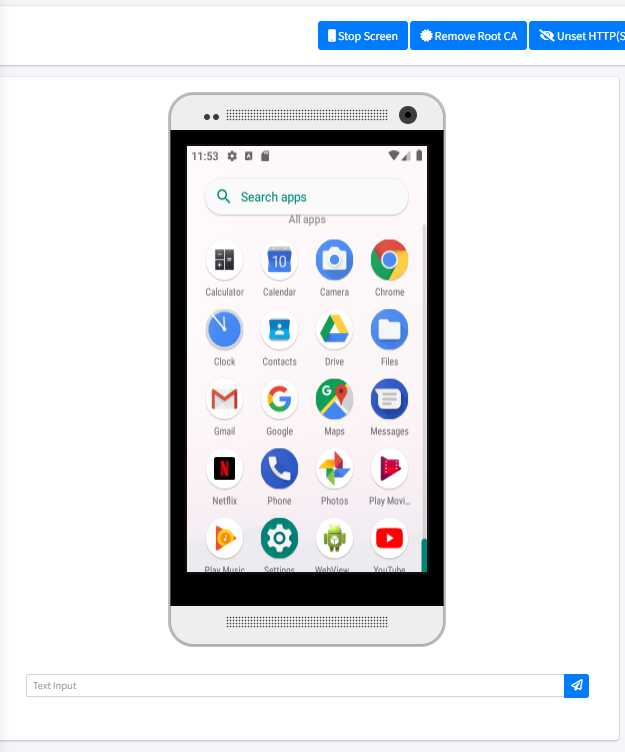
\includegraphics[width=1\linewidth]{Dynamic Analyzer/show_screen.jpg}
    \caption{Show Screen}
    \label{fig:example}
\end{figure}
\FloatBarrier
\subsection{Remove Root CA}
Removing the root CA in mobile security testing, such as with MobSF, disables HTTPS traffic interception during dynamic analysis. This action is often undertaken due to privacy concerns, legal restrictions, or application behavior constraints. It prevents the decryption of secure communications, potentially containing sensitive data. Root CA can be installed again.

\subsection{TLS/SSL Security Tester}
A TLS/SSL Security Tester evaluates the configuration and implementation of TLS/SSL protocols on servers or applications. It inspects protocol versions, cipher suites, and certificate validity to identify vulnerabilities. 
%will add image
\begin{figure}[hbt!]
    \centering
    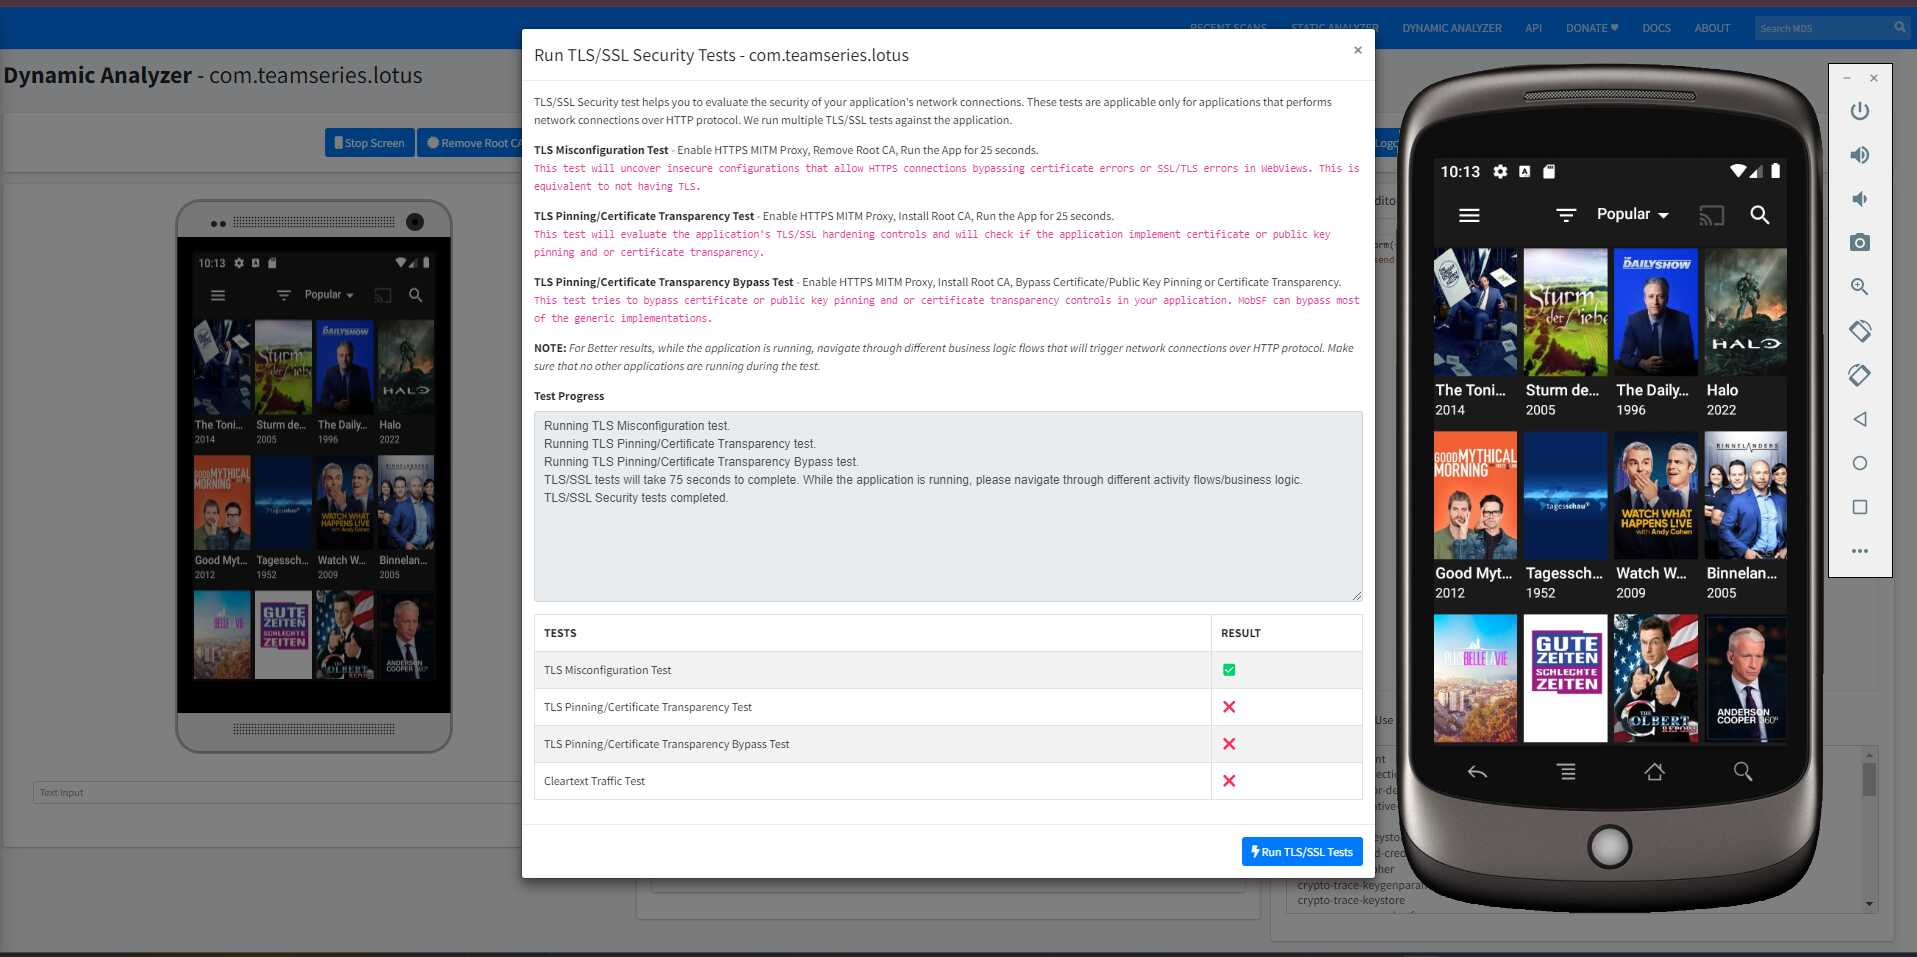
\includegraphics[width=1\linewidth]{Dynamic Analyzer/tsl.jpg}
    \caption{TLS/SSL Security Tester}
    \label{fig:example}
\end{figure}
\FloatBarrier

\subsection{Exported Activity Tester}
This feature allows MobSF to test the exported activities of the mobile application. In the background, MobSF will initiate each exported activity of the app and capture screenshots of their interfaces. This process aids in evaluating the functionality and behavior of the app's activities, providing insights into their appearance and functionality.

\subsection{Activity Tester}
The Activity Tester feature of MobSF launches every activity within the app and captures screenshots of each one. This thorough process ensures comprehensive testing coverage but may result in extended completion times, especially for complex applications. By capturing screenshots, analysts gain insights into the appearance and functionality of each activity, aiding in the detection of potential issues. 

% image
\begin{figure}[hbt!]
    \centering
    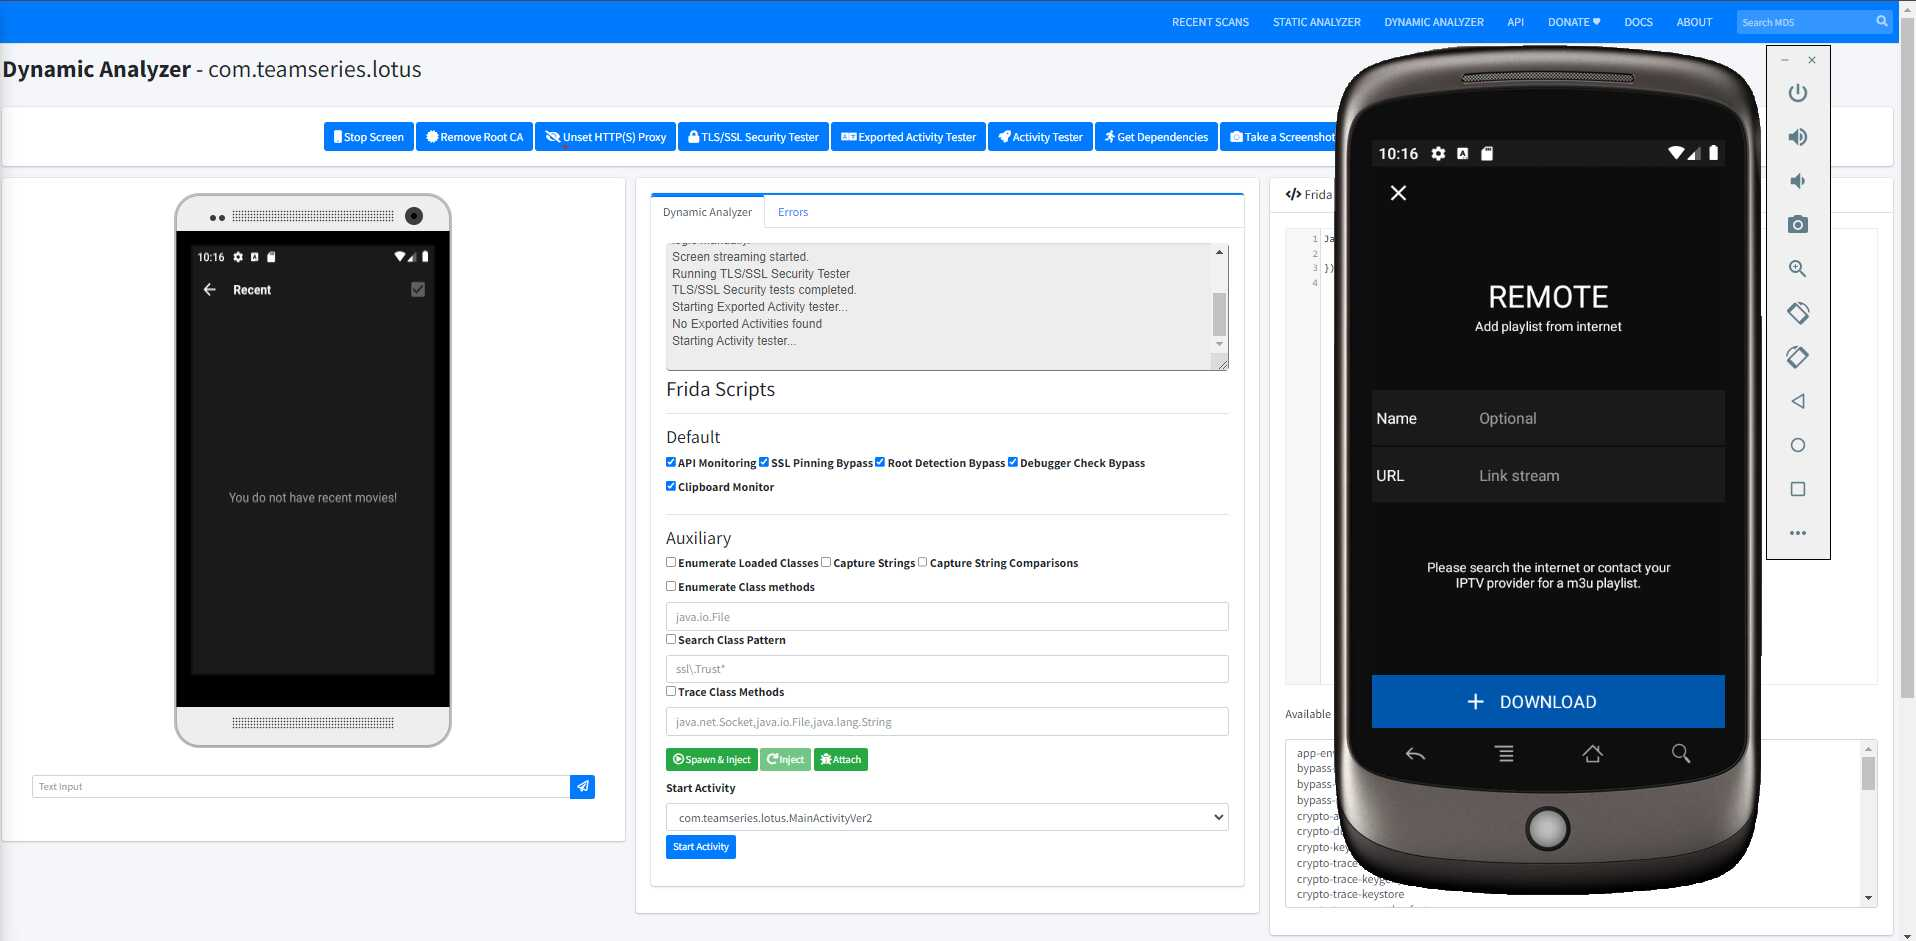
\includegraphics[width=1\linewidth]{Dynamic Analyzer/activitytester.jpg}
    \caption{Activity Tester}
    \label{fig:example}
\end{figure}
\FloatBarrier

\subsection{LogCat Stream}
The LogCat Stream feature opens a new window to display the live logcat stream of the mobile application. Logcat is a system log provided by Android devices that contains messages from various sources, including system processes, apps, and the Android operating system itself. By showing the logcat stream of the app, analysts can monitor real-time messages and events generated by the application during its execution. This visibility allows for the detection of errors, warnings, debug information, and other relevant events, facilitating troubleshooting, debugging, and security analysis of the application.

 %image
 \begin{figure}[hbt!]
    \centering
    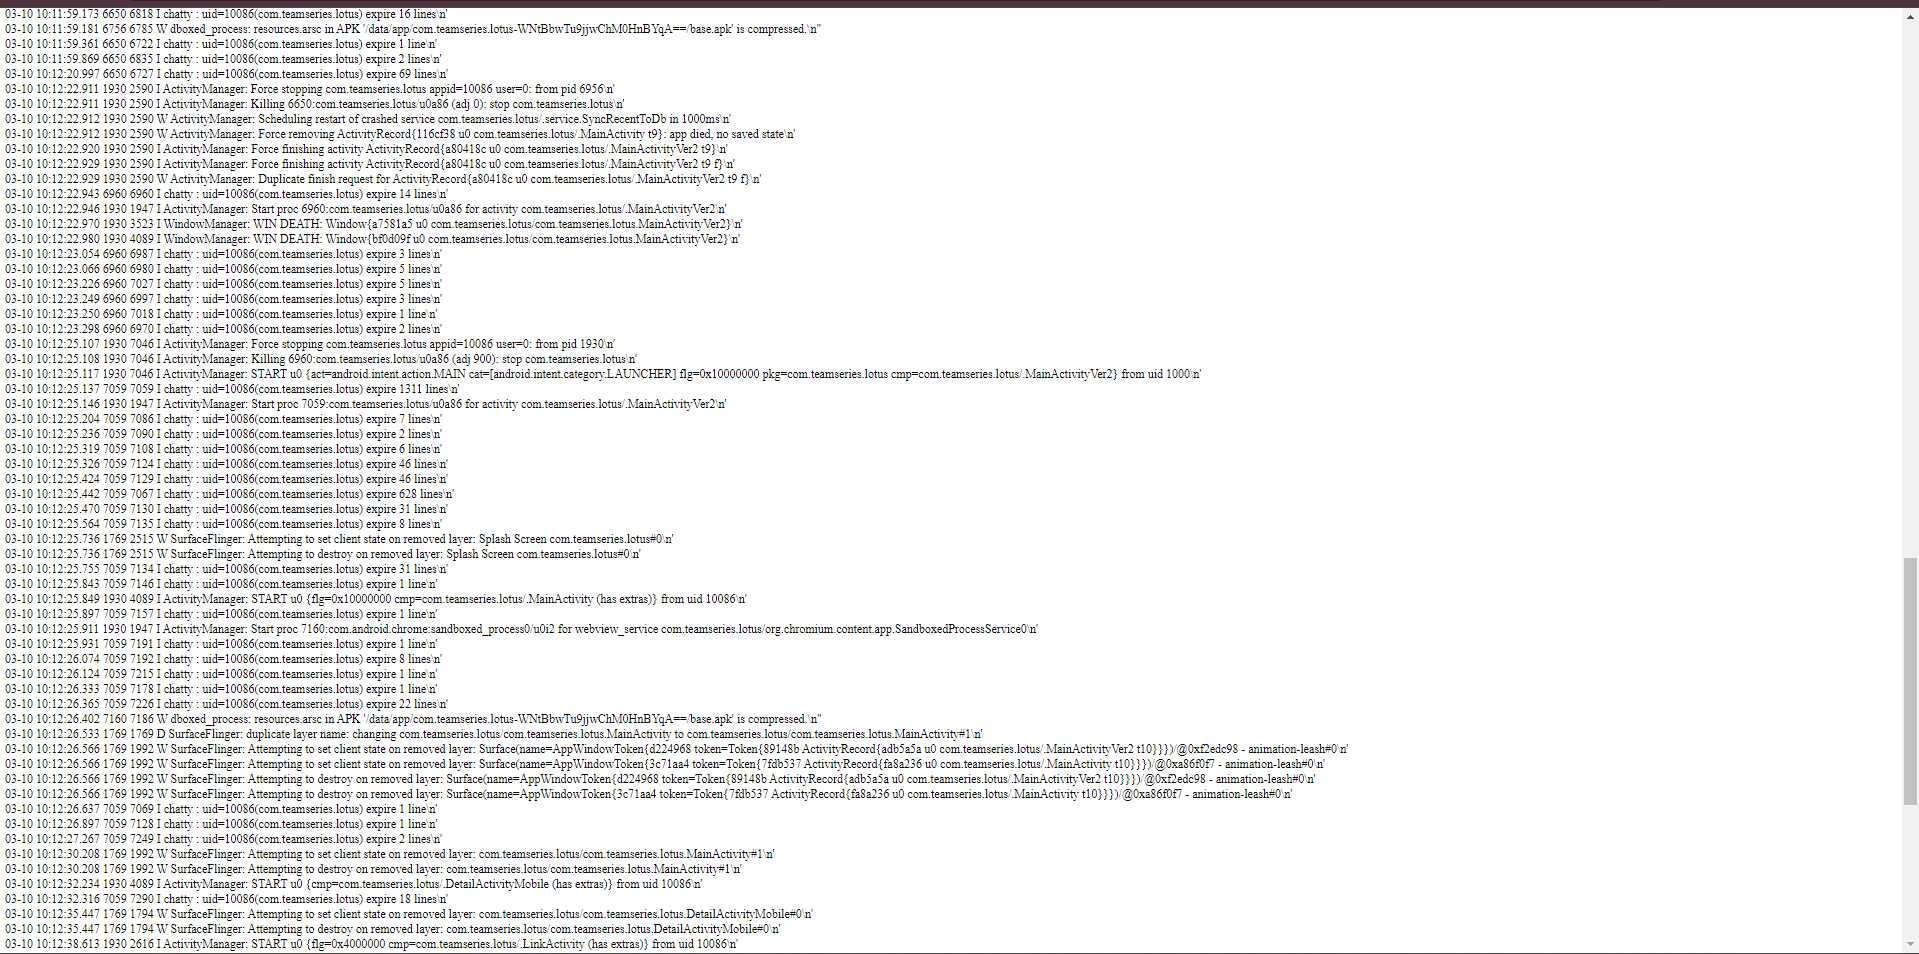
\includegraphics[width=1\linewidth]{Dynamic Analyzer/logcat.jpg}
    \caption{Logcat Stream}
    \label{fig:example}
\end{figure}
\FloatBarrier
 
\subsection{Live API Monitor}
The "Live API Monitoring" ssection in MobSF displays real-time API calls made by the app, aiding in understanding its functionality and interactions with external components like web services. This live monitoring offers insights into invoked functions, helping identify security issues, abnormal behavior, or unauthorized access. By observing API calls dynamically, analysts can detect malicious activities, assess adherence to security best practices, and pinpoint vulnerabilities efficiently. 

%% image
\begin{figure}[hbt!]
    \centering
    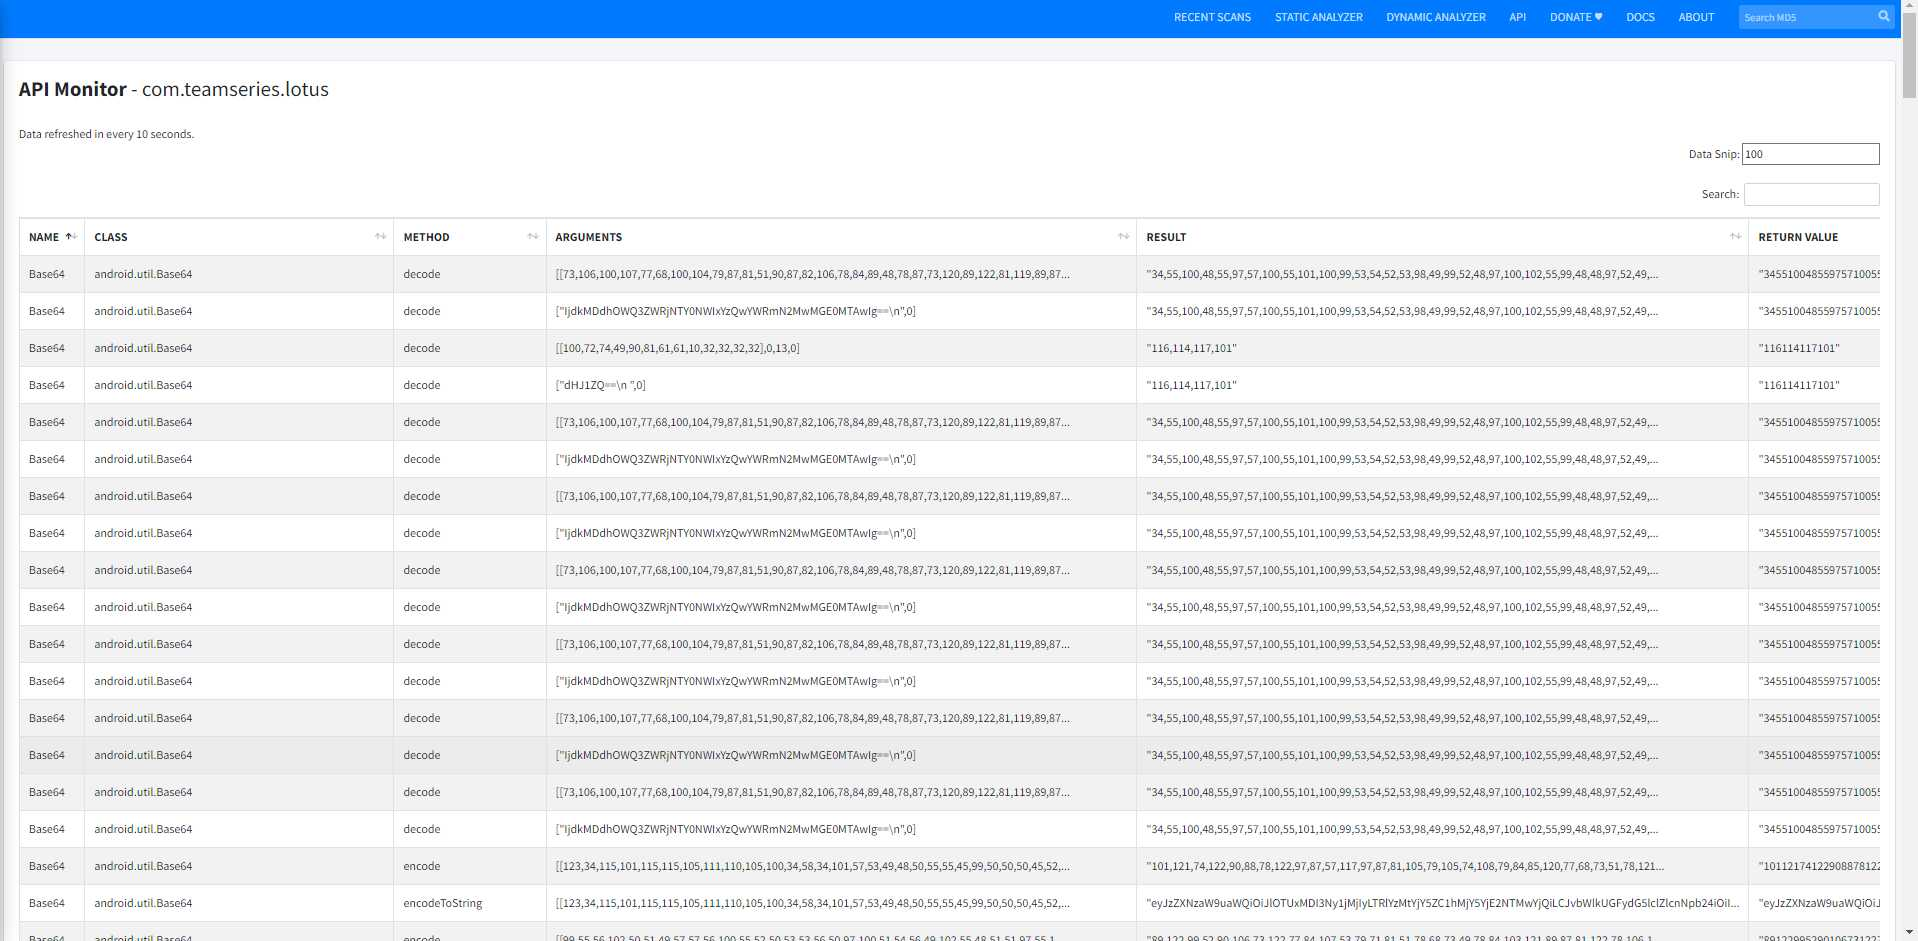
\includegraphics[width=1\linewidth]{Dynamic Analyzer/liveapimonitor.jpg}
    \caption{Live API Monitor}
    \label{fig:example}
\end{figure}
\FloatBarrier

\subsection{Frida Code Editor}
The Frida Code Editor feature in MobSF enables users to craft and upload custom Frida scripts for application analysis. This editor provides a dedicated space to write, modify, and debug scripts https://www.overleaf.com/project/6595b08ea0bacae28234d03etailored to specific testing objectives.
\begin{figure}[hbt!]
    \centering
    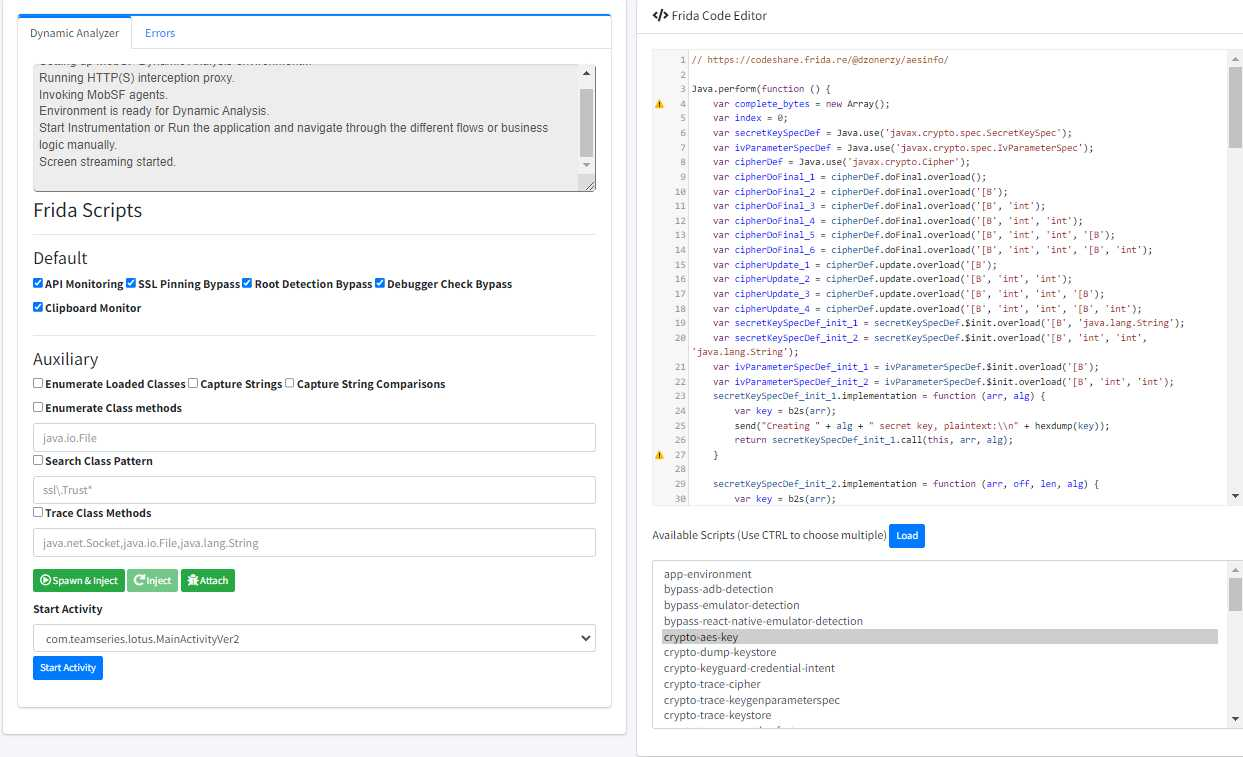
\includegraphics[width=1\linewidth]{Dynamic Analyzer/frida.jpg}
    \caption{Frida Code Editor}
    \label{fig:example}
\end{figure}
\FloatBarrier

\subsection{Shell Access}
There is also a shell access to the emulator.Which can run adb commands.

\subsection{Generate Report}
Report contains the following sections-
\begin{figure}[hbt!]
    \centering
    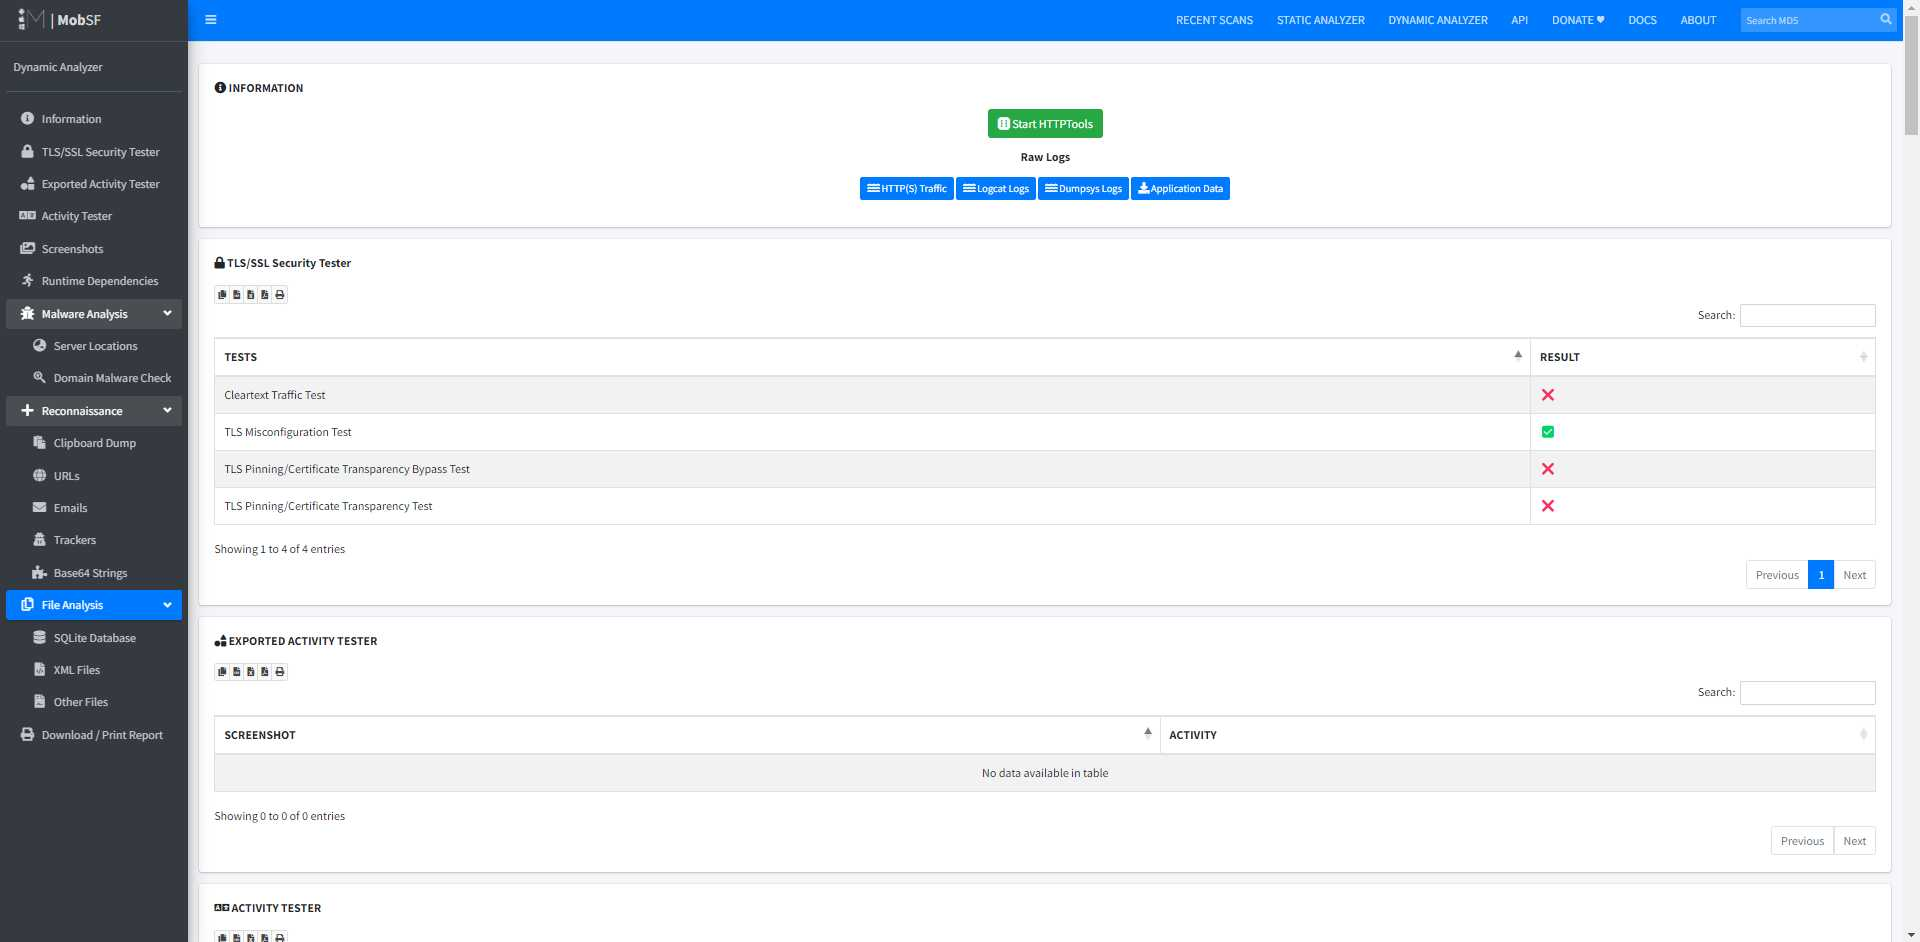
\includegraphics[width=1\linewidth]{Dynamic Analyzer/generate_report.jpg}
    \caption{Reports}
    \label{fig:example}
\end{figure}
\FloatBarrier

\subsubsection{Information}
Information contains "startHTTPTools" section. "startHTTPTools" triggers functionalities related to analyzing HTTP traffic during runtime. This could include launching an HTTP proxy server to intercept and analyze HTTP requests and responses, enabling sniffing capabilities to monitor network traffic, and activating modules for analyzing and fuzzing HTTP communication for security vulnerabilities.

Report Section looks like this-
\begin{figure}[hbt!]
    \centering
    
\includegraphics[width=1\linewidth]{Dynamic Analyzer/info.jpg}
    \caption{Activity Tester}
    \label{fig:example}
\end{figure}
\FloatBarrier

\subsubsection{TLS/SSL Security Tester}
The TLS/SSL Tester in MobSF encompasses several critical tests for evaluating the security posture of TLS/SSL implementations within applications:
\begin{itemize}

\item \textbf{Cleartext Traffic Test:} This test examines whether the application sends sensitive data over unencrypted, cleartext channels. Detecting such behavior is crucial for identifying potential security risks, such as data leakage or interception by malicious actors.

\item \textbf{TLS Misconfiguration Test:} This test assesses the configuration of the TLS protocol used by the application. It checks for common misconfigurations that could weaken the security of TLS connections, such as outdated cipher suites, insecure protocol versions, or improper certificate validation settings.

\item \textbf{TLS Pinning/Certificate Transparency Bypass Test:} This test focuses on bypassing TLS pinning mechanisms implemented by the application. It evaluates the effectiveness of certificate pinning and verifies whether the application properly enforces trust only for predefined certificates, preventing potential attacks that rely on certificate manipulation.

\item \textbf{TLS Pinning/Certificate Transparency Test:} This test verifies the implementation of TLS pinning and certificate transparency mechanisms within the application. It ensures that the application correctly validates server certificates against predefined trust anchors and checks for the presence of certificates in public certificate transparency logs, enhancing the overall security of TLS connections.

\end{itemize}

\begin{figure}[hbt!]
    \centering
    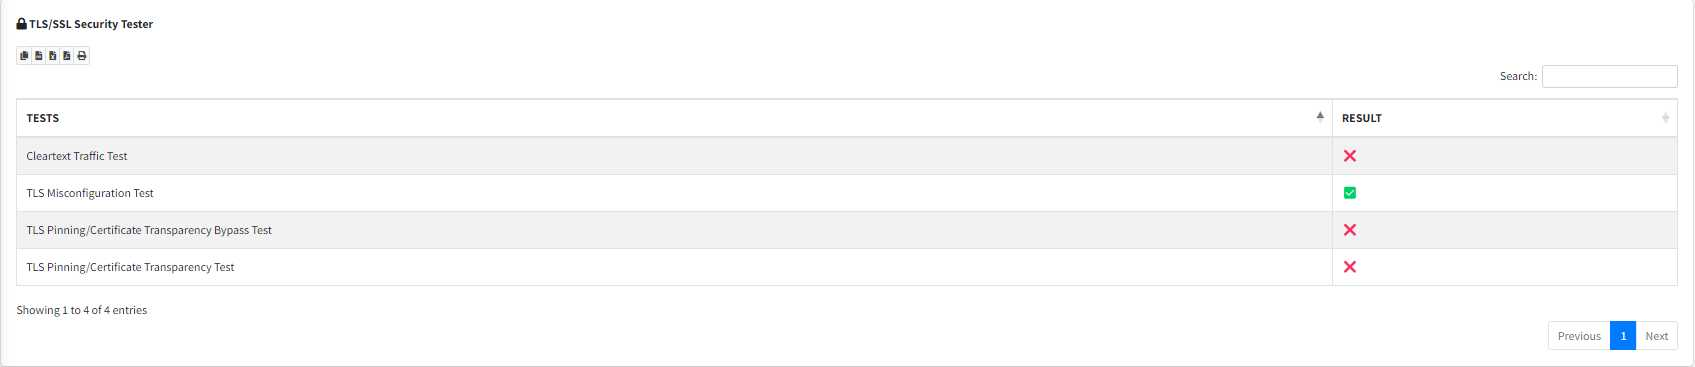
\includegraphics[width=1\linewidth]{Dynamic Analyzer/tls_rep.jpg}
    \caption{TLS/SSL Security Tester}
    \label{fig:example}
\end{figure}
\FloatBarrier

\subsubsection{Exported Activity Tester}

This allows MobSF to test the exported activities of the mobile application. In the background, MobSF will initiate each exported activity of the app and capture screenshots of their interfaces. This process aids in evaluating the functionality and behavior of the app's activities, providing insights into their appearance and functionality.
\begin{figure}[hbt!]
    \centering
    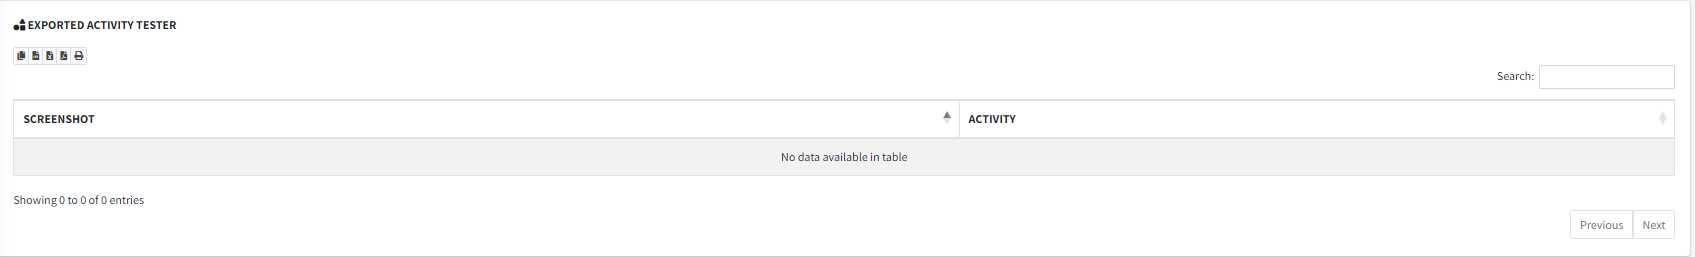
\includegraphics[width=1\linewidth]{Dynamic Analyzer/exported_rep.jpg}
    \caption{Exported Activity Tester}
    \label{fig:example}
\end{figure}
\FloatBarrier

\subsubsection{Activity Tester}
The Activity Tester launches every activity within the app and captures screenshots of each one. This thorough process ensures comprehensive testing coverage but may result in extended completion times, especially for complex applications. By capturing screenshots, analysts gain insights into the appearance and functionality of each activity, aiding in the detection of potential issues. 
\begin{figure}[hbt!]
    \centering
    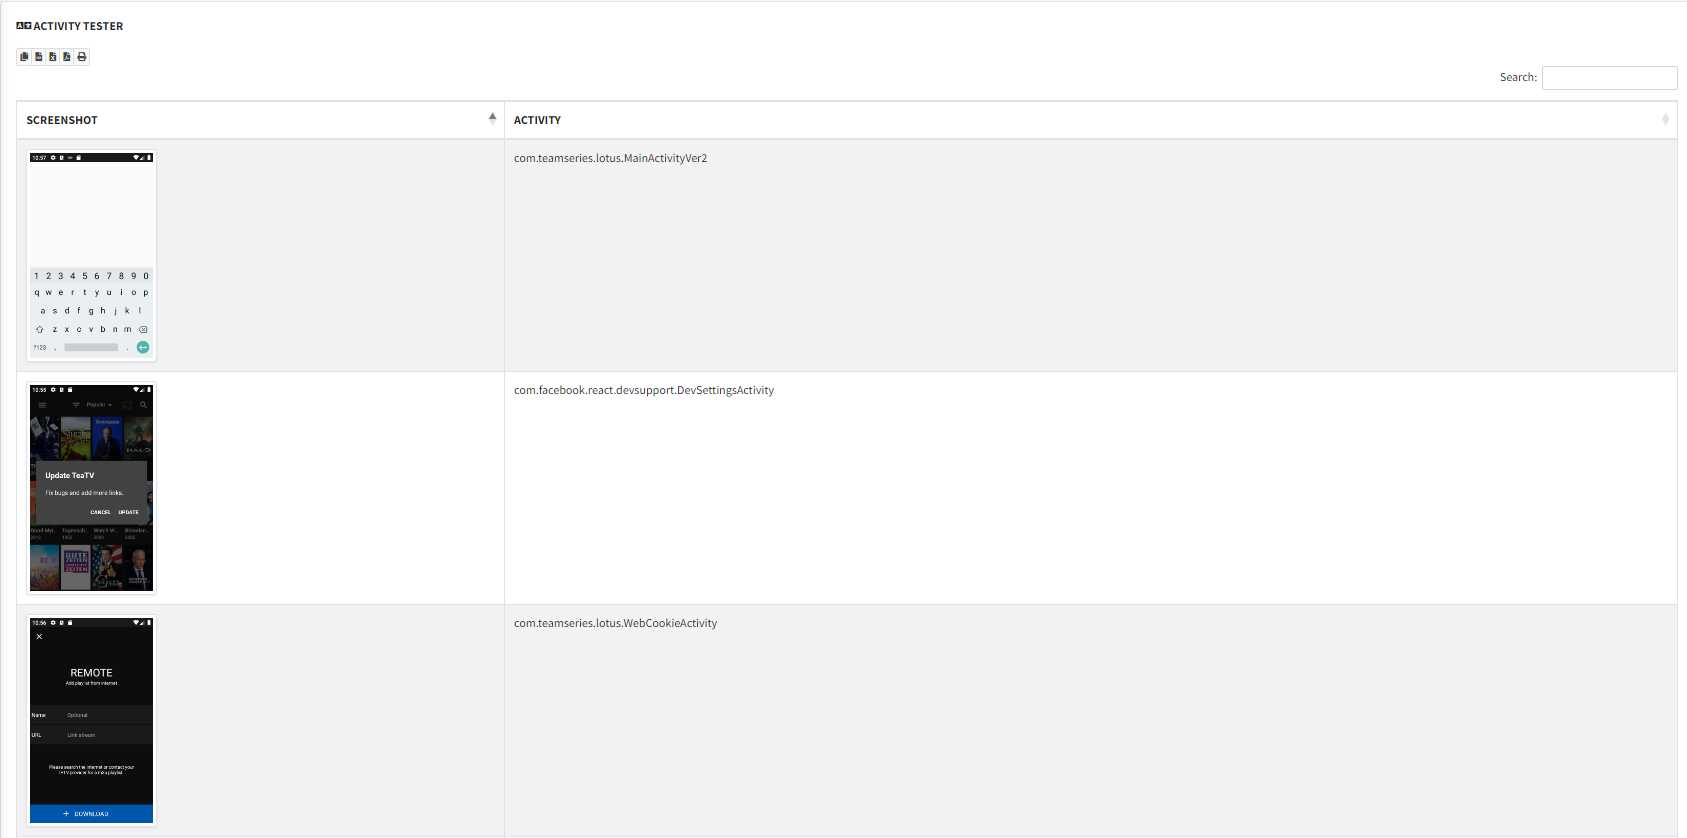
\includegraphics[width=1\linewidth]{Dynamic Analyzer/activity_rep.jpg}
    \caption{Activity Tester}
    \label{fig:example}
\end{figure}
\FloatBarrier

\subsubsection{Screenshots}
Shows screenshots of activities during runtime.


\subsubsection{Runtime Dependencies}
In MobSF's dynamic analysis, runtime dependencies include third-party libraries, system APIs, and network services critical for app functionality. MobSF scrutinizes how apps interact with these dependencies to uncover security risks like insecure data transmission or improper API usage. By evaluating runtime dependencies, MobSF aids in identifying vulnerabilities introduced by outdated libraries or insecure interactions. It ensures compliance with security standards, enhances app security, and guides informed decisions on dependency management.

\subsection{Malware Analysis}
It has two sections-
\begin{itemize}
    \item \textbf {Server Locations: } Server locations in MobSF's dynamic analysis reveal the geographic hosting of app servers, pivotal for privacy, compliance, and security evaluations. By scrutinizing server locations, MobSF assesses data residency compliance, detects potential data leakage, and evaluates security risks associated with server communication.
    \begin{figure}[hbt!]
    \centering
    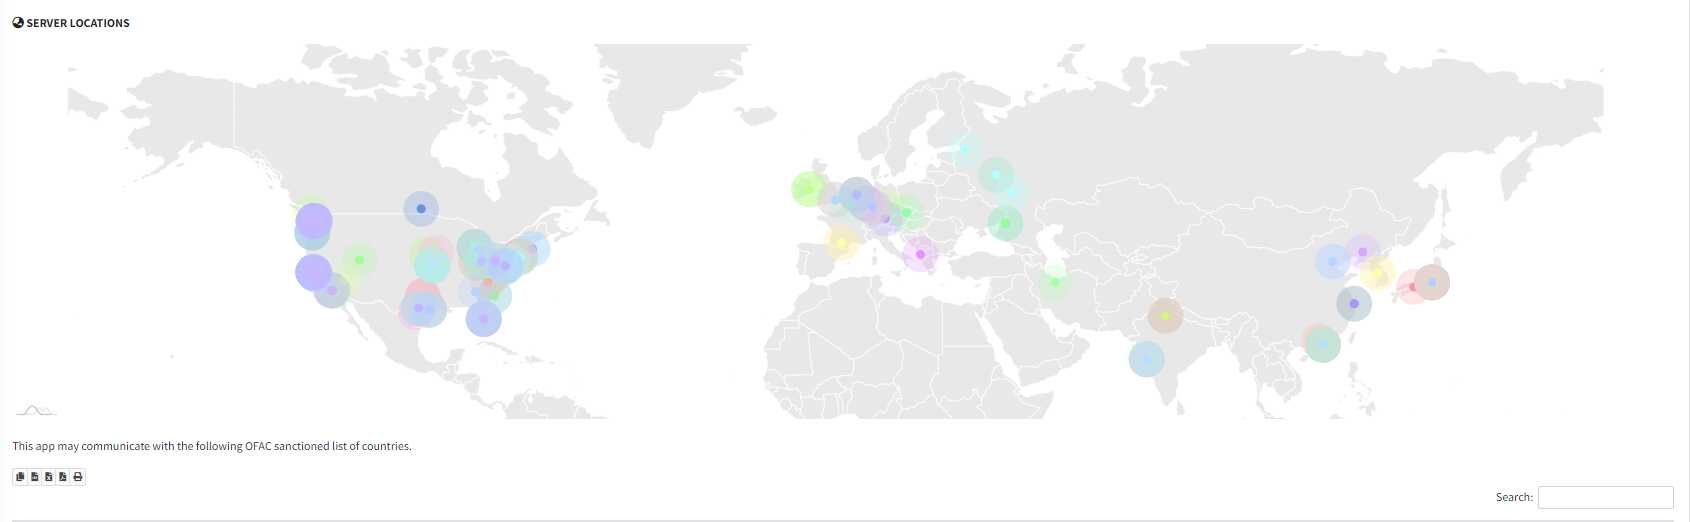
\includegraphics[width=0.5\linewidth]{Dynamic Analyzer/server_rep.jpg}
    \caption{Server Locations}
    \label{fig:example}
    \end{figure}
    \FloatBarrier

    \begin{figure}[hbt!]
    \centering
    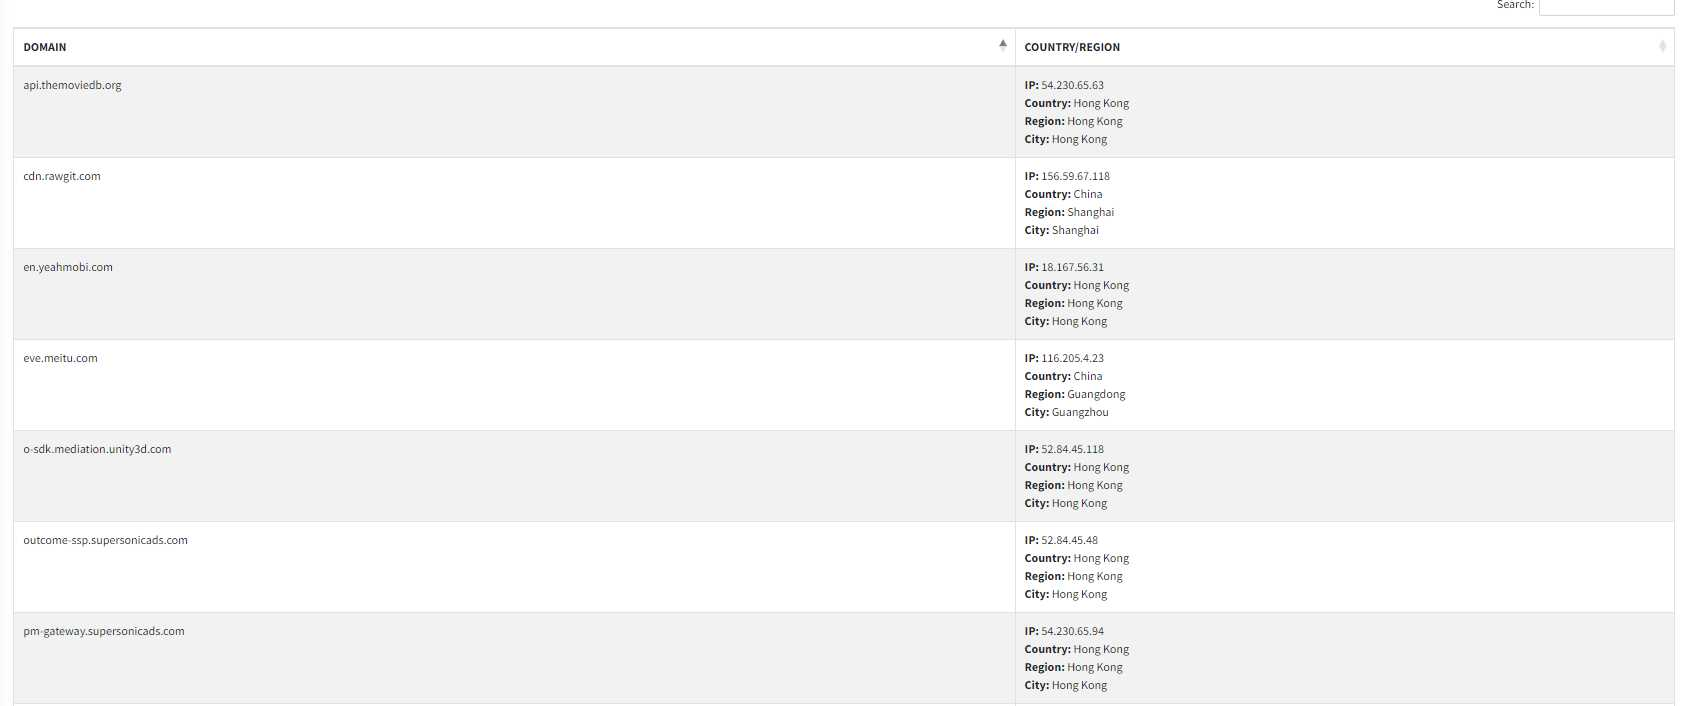
\includegraphics[width=0.5\linewidth]{Dynamic Analyzer/server_rep2.jpg}
    \caption{Server Locations}
    \label{fig:example}
    \end{figure}
    \FloatBarrier
    
    \item \textbf {Domain Malware Check: }
    Domain Malware Check is a feature within MobSF's dynamic analysis toolkit designed to inspect domains accessed by the mobile application for potential malware or malicious activity. During runtime, MobSF scrutinizes the URLs or domains contacted by the app, cross-referencing them with known malware databases and blacklists. This process helps identify suspicious domains associated with malware distribution, phishing attempts, or other malicious activities.
    \begin{figure}[hbt!]
    \centering
    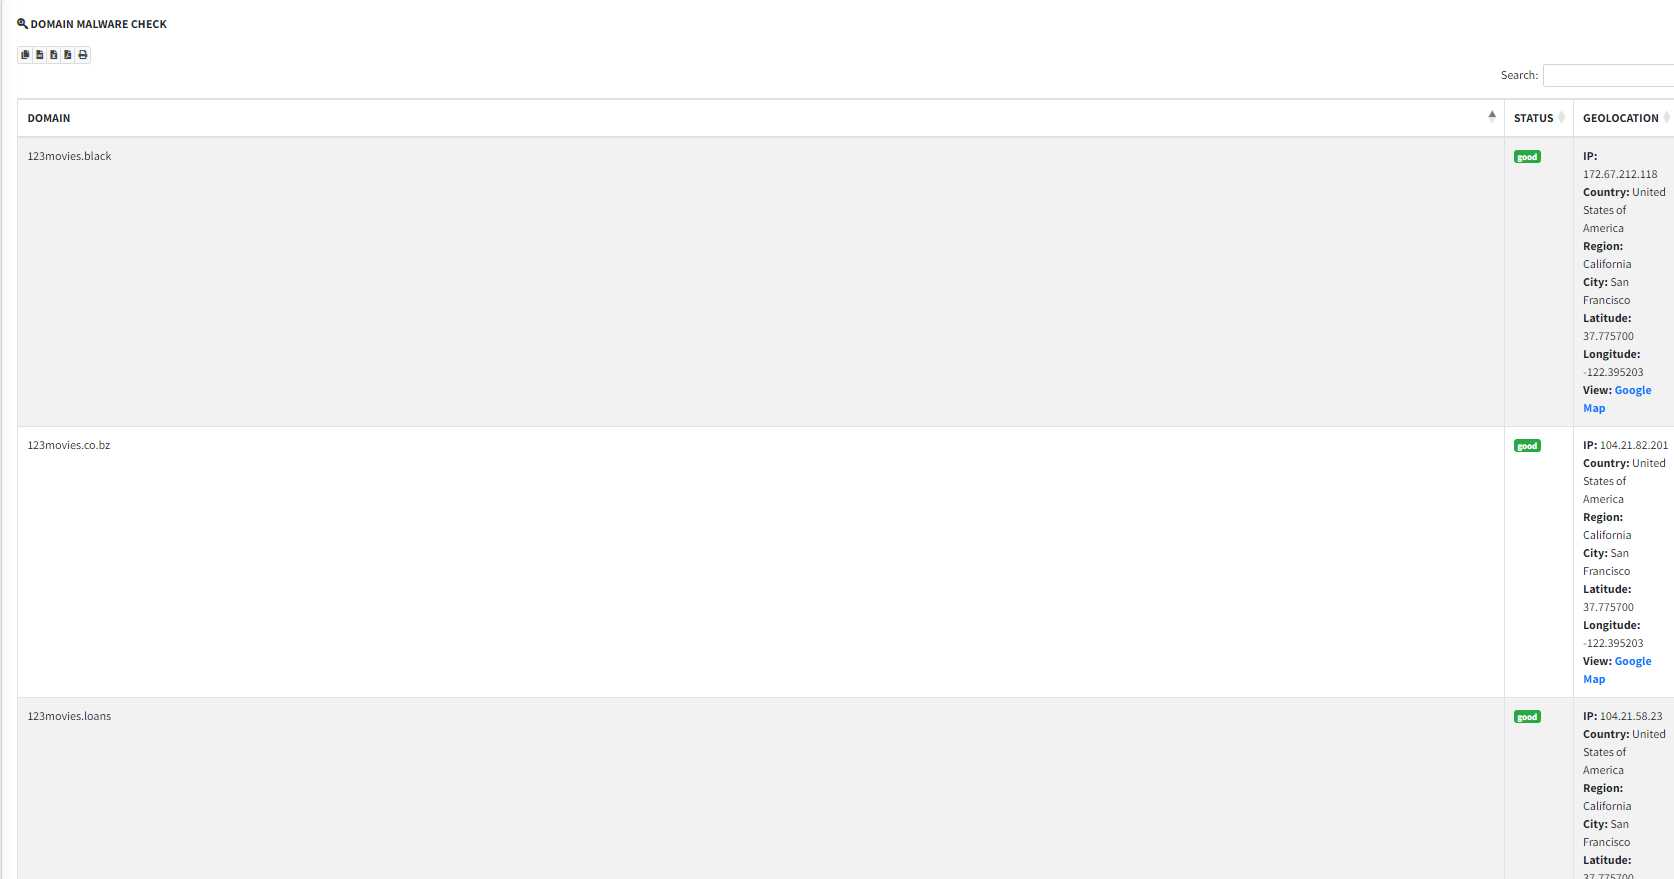
\includegraphics[width=1\linewidth]{Dynamic Analyzer/domain_mal_rep.jpg}
    \caption{Domain Malware Check}
    \label{fig:example}
    \end{figure}
    \FloatBarrier

    
\end{itemize}

\subsubsection{Reconnaissance}
It has following sections:
\begin{itemize}
    \item \textbf {Clipboard dump: } Shows any clipboard dumps while running app.
    \item \textbf {URLs : }This section focuses on analyzing the URLs or domains accessed by the mobile application during runtime, providing insights into its network behavior and potential security risks associated with external communication
    \item \textbf {Emails : } SHows emails accessed during runtime. 
    \begin{figure}[hbt!]
    \centering
    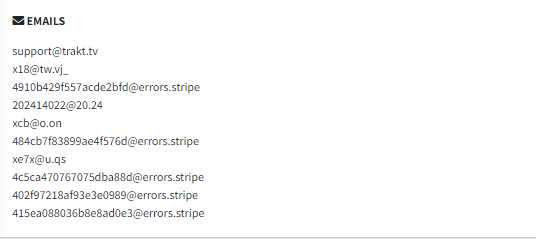
\includegraphics[width=1\linewidth]{Dynamic Analyzer/email_rep.jpg}
    \caption{Email}
    \label{fig:example}
    \end{figure}
    \FloatBarrier

    \item \textbf {Trackers : }Refers to third-party components in mobile apps that collect user data, monitor behavior, or serve ads. MobSF analyze trackers by identifying their presence, scrutinizing data collection behavior, assessing privacy risks, and ensuring regulatory compliance.
    \begin{figure}[hbt!]
    \centering
    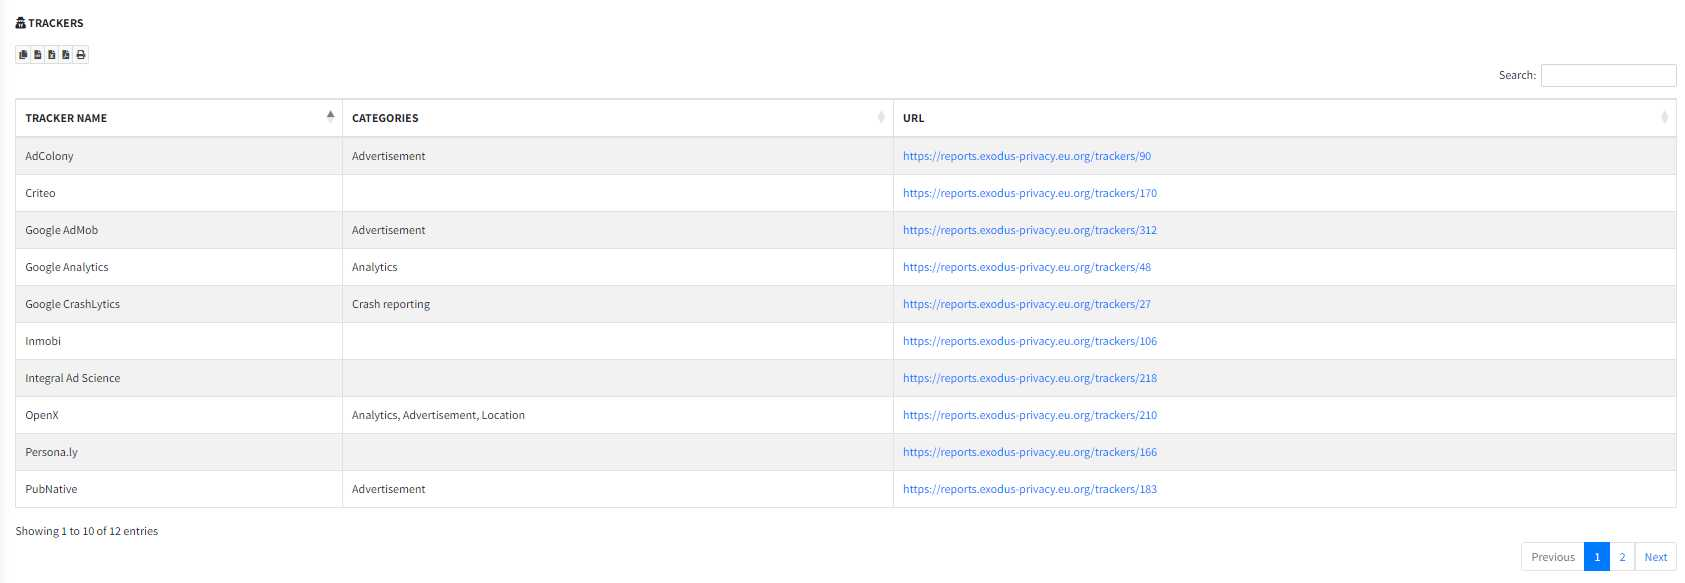
\includegraphics[width=1\linewidth]{Dynamic Analyzer/trackers_rep.jpg}
    \caption{Trackers}
    \label{fig:example}
    \end{figure}
    \FloatBarrier
    

    \item \textbf{Base64 Strings}
    Shows base64 strings used during runtime. 

\end{itemize}

\subsubsection{File Analysis}
\begin{itemize}
    \item \textbf {SQLite Database : }In dynamic analysis, SQLite databases in mobile apps undergo scrutiny. This involves analyzing the database schema, extracting stored data, and assessing data manipulation. Examining how the app interacts with SQLite reveals its functionality and security measures, such as encryption and access controls. 
    \begin{figure}[hbt!]
    \centering
    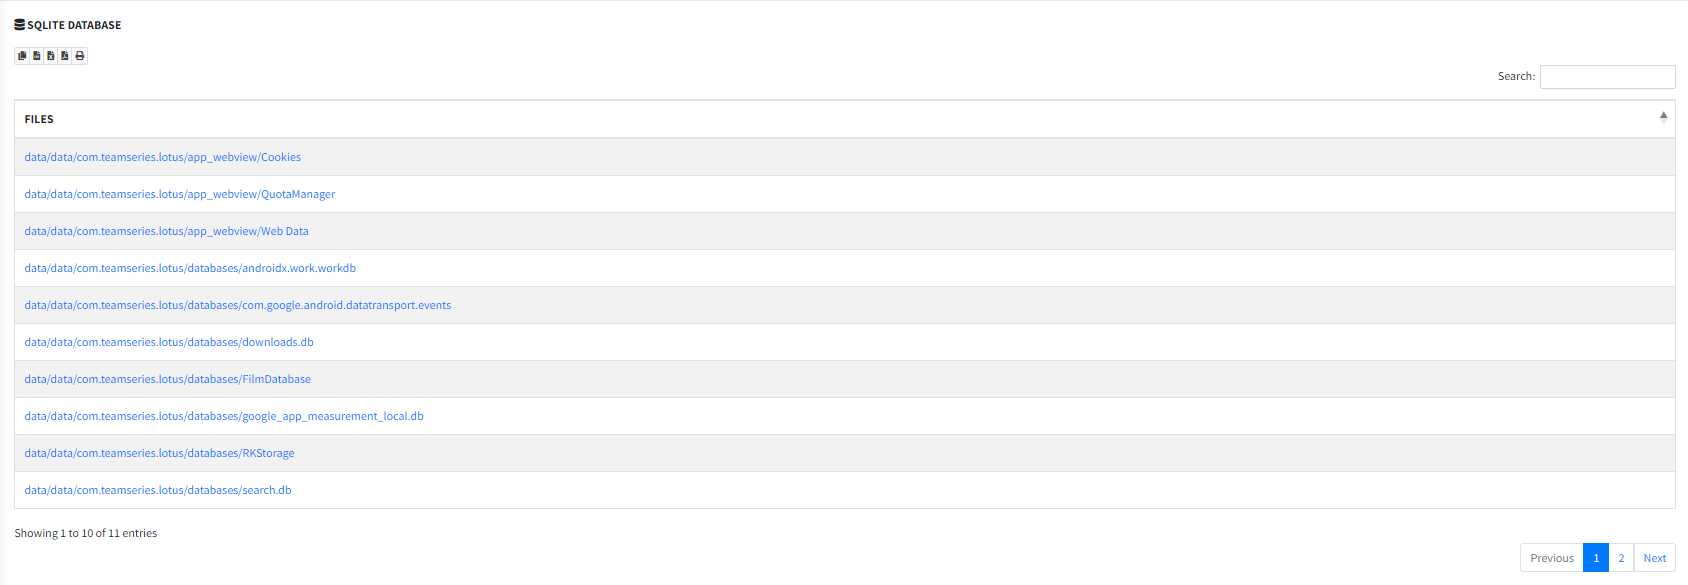
\includegraphics[width=1\linewidth]{Dynamic Analyzer/sqlite.jpg}
    \caption{SQLite Database}
    \label{fig:example}
    \end{figure}
    \FloatBarrier

    \item \textbf {XML Files : }
    XML files in mobile app dynamic analysis, such as with MobSF, reveal crucial information about app structure, configurations, and communication protocols. Analyzing AndroidManifest.xml unveils permissions and components. Inspection of layout and configuration XMLs uncovers UI design and settings. Examination of XMLs for hardcoded URLs aids in assessing security risks. 
    \begin{figure}[hbt!]
    \centering
    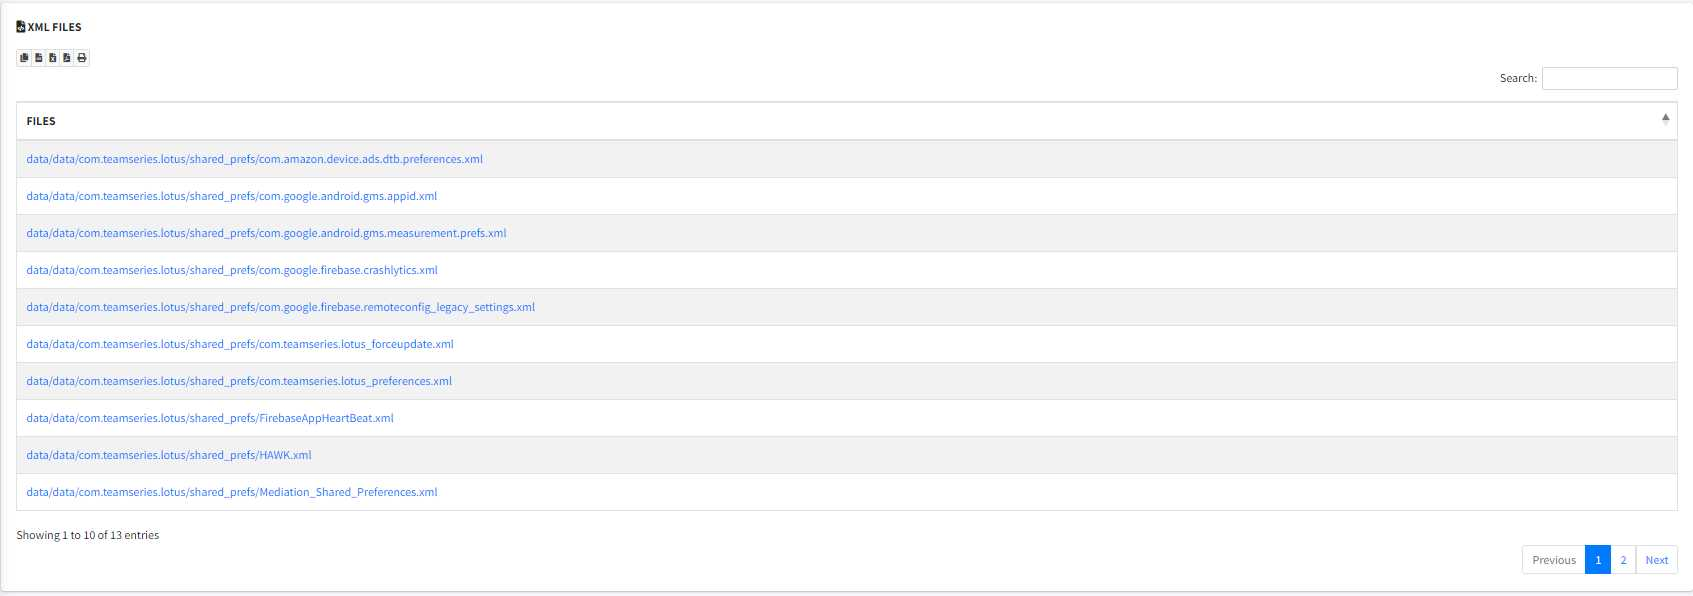
\includegraphics[width=1\linewidth]{Dynamic Analyzer/xml.jpg}
    \caption{XML FIles}
    \label{fig:example}
    \end{figure}
    \FloatBarrier

    \item \textbf{Other Files : } Show other files accessed during runtime. 
    \begin{figure}[hbt!]
    \centering
    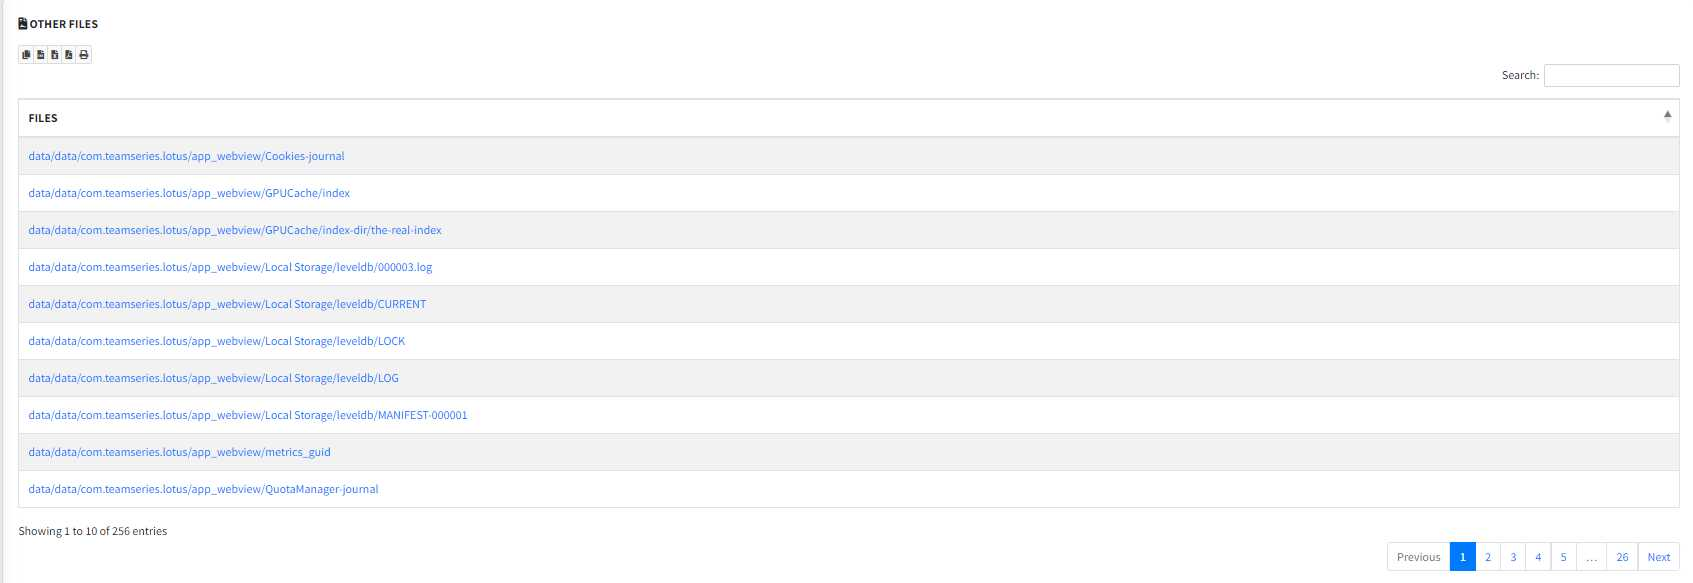
\includegraphics[width=1\linewidth]{Dynamic Analyzer/others.jpg}
    \caption{Other Files}
    \label{fig:example}
    \end{figure}
    \FloatBarrier
\end{itemize}
\chapter{Codebase}
The whole code can be found in the github link \url{https://github.com/MobSF/Mobile-Security-Framework-MobSF}. Inside the repository, we have a folder named "mobsf". The backbone codes are mostly in this folder. Some of the prominent folders are listed below along with the explanation of their codes.
\section{MobSF}
Inside the MObSF folder, we have a views folder and some files-
\begin{itemize}
    \item \textbf\textbf{utils.py :} Some utility functions are present here.    
    \item \textbf\textbf{urls.py :} file is defining the URL patterns specifically for the Mobile Security Framework (MobSF) Django application.
    % \begin{figure}[hbt!]
    %     \centering
    %     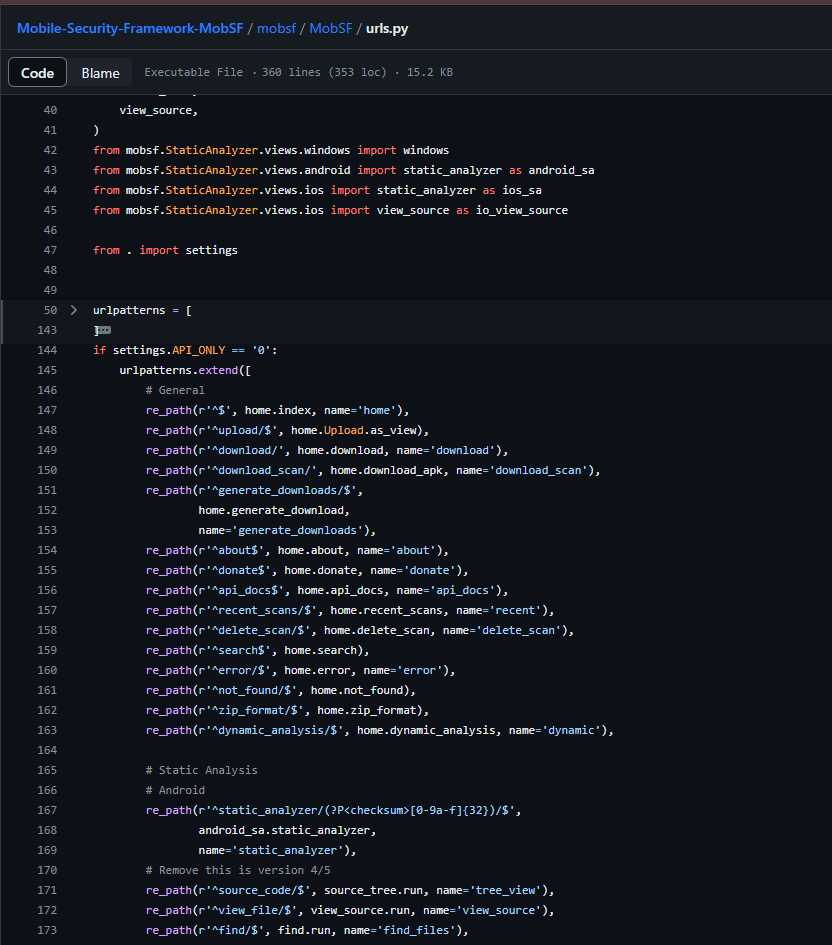
\includegraphics[width=0.5\linewidth]{MobSF/urlspy.jpg}
    %     \caption{urls.py}
    %     \label{fig:example}
    % \end{figure}
    % \FloatBarrier
    \item \textbf\textbf{settings.py :} 
    This settings.py file for MobSF's Django project configures directories, databases, middleware, URLs, and enterprise features. It also loads user configurations and sets up logging, allowing customization and control over the application's behavior and interactions with external resources.
    % \begin{figure}[hbt!]
    %     \centering
    %     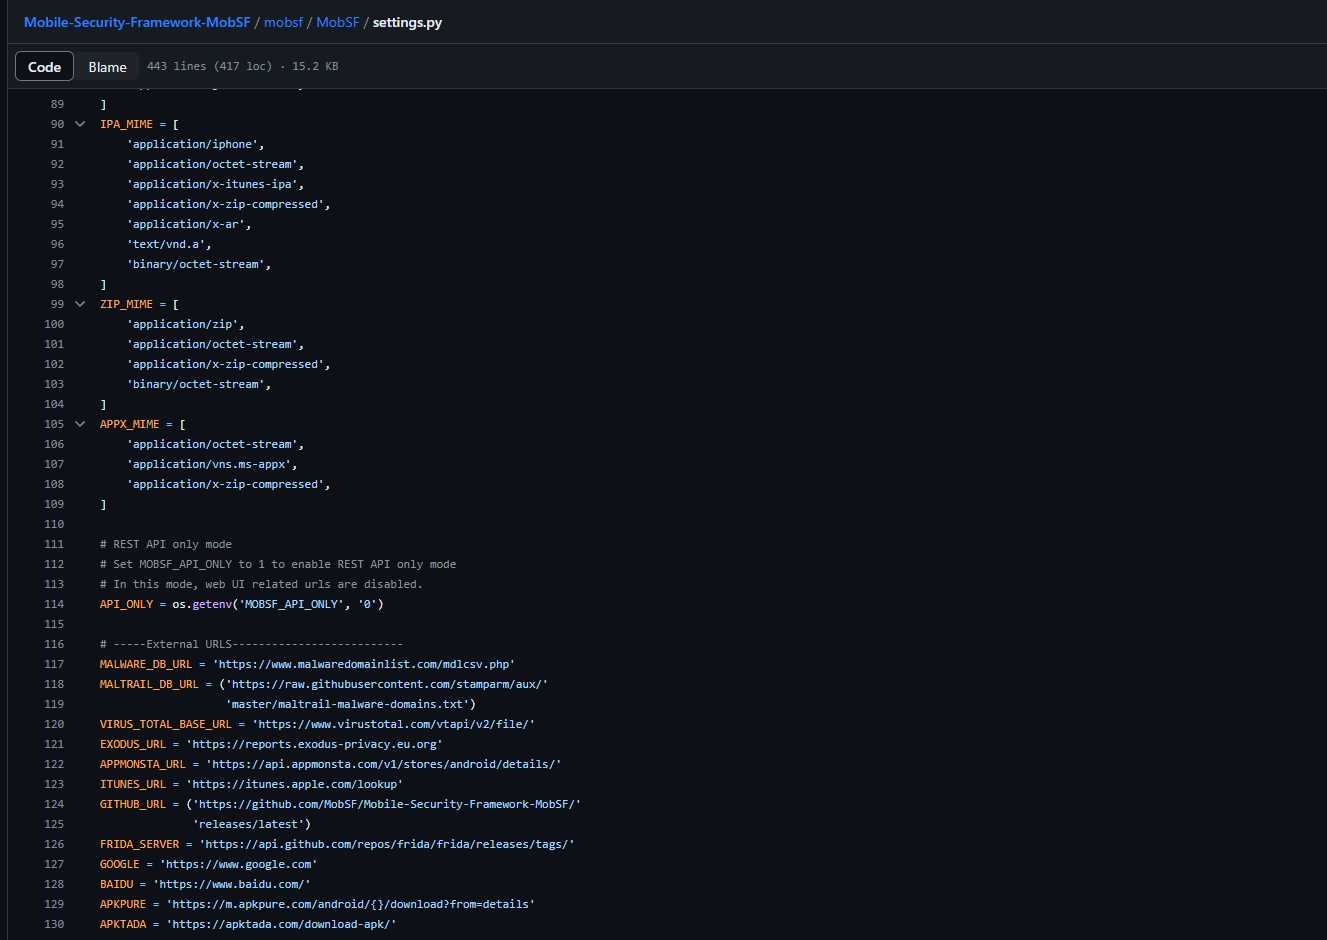
\includegraphics[width=0.8\linewidth]{MobSF/settings.jpg}
    %     \caption{settings.py}
    %     \label{fig:example}
    % \end{figure}
    % \FloatBarrier
    \item \textbf\textbf{security.py :} This script in MobSF detects tampering with runtime executables. It calculates SHA-256 hashes of files, checks for changes during execution, and logs discrepancies.
    % \begin{figure}[hbt!]
    %     \centering
    %     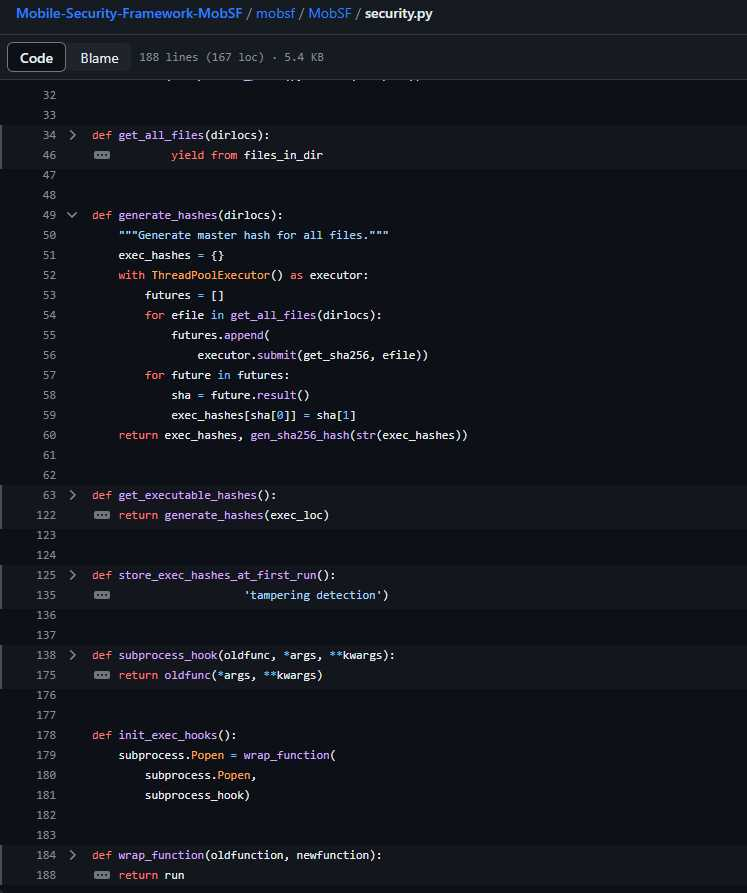
\includegraphics[width=0.6\linewidth]{MobSF/securitypng.jpg}
    %     \caption{settings.py}
    %     \label{fig:example}
    % \end{figure}
    % \FloatBarrier
    \item \textbf\textbf{init.py :}
    This script initializes MobSF on first run by generating a secret key, creating necessary directories, and performing database migrations.
    % \begin{figure}[hbt!]
    %     \centering
    %     \includegraphics[width=0.6\linewidth]{MobSF/initpy.jpg}
    %     \caption{init.py}
    %     \label{fig:example}
    % \end{figure}
    % \FloatBarrier
    \item \textbf\textbf{forms.py :}This script defines a Django form for uploading files and a utility class for handling form errors and returning them in a specific format.
    % \begin{figure}[hbt!]
    %     \centering
    %     \includegraphics[width=0.6\linewidth]{MobSF/formspy.jpg}
    %     \caption{forms.py}
    %     \label{fig:example}
    % \end{figure}
    % \FloatBarrier


    \item \textbf{views folder}
    \begin{itemize}
        \item \textbf\textbf {apkdownloader.py :}This script is for downloading Android APK files from various sources. It includes functions to fetch HTML content from URLs, download files, determine the type of APK file (regular APK or split APK), and add APK files to MobSF (Mobile Security Framework). The apk\_download function is the main entry point, attempting to download an APK file based on the provided package name.
        % \begin{figure}[hbt!]
        %     \centering
        %     \includegraphics[width=0.6\linewidth]{MobSF/views/apkdownloader.jpg}
        %     \caption{apkdownloader.py}
        %     \label{fig:example}
        %     \end{figure}
        % \FloatBarrier
        
        \item \textbf\textbf {helpers.py :}
        The code snippet provides two key functionalities for a Django application. Firstly, the FileType class helps identify file types based on their content type and name. It offers methods to determine if a file type is allowed, such as checking for APKs, SO files, or ZIP archives. Secondly, the request\_method decorator ensures that a view function only responds to HTTP request methods specified in a list or tuple. If the incoming request method is not allowed, it returns a "405 Method Not Allowed" response. These utilities enhance file handling and enforce HTTP method constraints in the Django application.
        % \begin{figure}[hbt!]
        %     \centering
        %     \includegraphics[width=0.6\linewidth]{MobSF/views/helpers.jpg}
        %     \caption{helpers.py}
        %     \label{fig:example}
        %     \end{figure}
        % \FloatBarrier
        \item \textbf\textbf {home.py :}
        
        \begin{itemize}
        This Python code implements Django views and utility functions for handling file uploads, managing API routes, and rendering HTML templates for different pages in a web application. Key features include:
            \item \textbf{Index Route:} Displays the home page of the application.
            \item \textbf{Upload:} Handles file uploads, distinguishing between different file types such as APK, IPA, JAR, etc., and initiates scanning based on the file type.
            \item \textbf{API Docs, About, Donate, Error, Zip Format, Dynamic Analysis, Not Found:} Routes for displaying various static pages like API documentation, about page, donation page, etc.
            \item \textbf{Recent Scans:} Renders a page showing the recently scanned files with their details.
            \item \textbf{Download APK:} Allows downloading APK files based on the provided package name.
            \item \textbf{Search:} Enables searching for a particular scan by its MD5 hash.
            \item \textbf{Download:} Handles file download requests, ensuring security checks to prevent path traversal attacks.
            \item \textbf{Generate Download:} Generates downloads for uploaded binaries or source code files.
            \item \textbf{Delete Scan:} Deletes a scan from the database along with related files.
            \item \textbf{Recent Scans:} Provides functionality to paginate and retrieve recent scan data.
            % \begin{figure}[hbt!]
            %     \centering
            %     \includegraphics[width=0.6\linewidth]{MobSF/views/home.jpg}
            %     \caption{home.py}
            %     \label{fig:example}
            % \end{figure}
            % \FloatBarrier
        \end{itemize}

        \item \textbf{scanning.py :}
        This Python code defines a class Scanning and some helper functions to handle file uploads and static analysis of different file types in the MobSF (Mobile Security Framework) application. Here's an explanation of the code:
        \begin{itemize}
          \item \textbf \texttt{add\_to\_recent\_scan(data)}:
          \begin{itemize}
            \item \textbf Adds information about a scanned file to the database under the Recent Scan model.
          \end{itemize}
          
          \item \textbf \texttt{handle\_uploaded\_file(content, extension)}:
          \begin{itemize}
            \item \textbf Writes the uploaded file to the server's file system and returns its MD5 hash. It's used to handle different types of file uploads.
          \end{itemize}
          
          \item \textbf{Scanning Class Initialization:}
          \begin{itemize}
            \item \textbf Initializes the Scanning object with the uploaded file and its name obtained from the request.
          \end{itemize}
          
          \item \textbf{Scanning Class Methods:}
          \begin{itemize}
            \item \textbf \texttt{scan\_apk}: Handles static analysis of Android APK files.
            \item \textbf \texttt{scan\_xapk}: Handles static analysis of Android XAPK files.
            \item \textbf \texttt{scan\_apks}: Handles static analysis of Android Split APK files.
            \item \textbf \texttt{scan\_jar}: Handles static analysis of Java JAR files.
            \item \textbf \texttt{scan\_aar}: Handles static analysis of Android AAR files.
            \item \textbf \texttt{scan\_so}: Handles static analysis of shared object files.
            \item \textbf \texttt{scan\_zip}: Handles static analysis of zipped Android/iOS source code files.
            \item \textbf \texttt{scan\_ipa}: Handles static analysis of iOS IPA files.
            \item \textbf \texttt{scan\_dylib}: Handles static analysis of iOS Dylib files.
            \item \textbf \texttt{scan\_a}: Handles static analysis of static library files.
            \item \textbf \texttt{scan\_appx}: Handles static analysis of Windows appx files.
          \end{itemize}
        \end{itemize}
        % \begin{figure}[hbt!]
        %         \centering
        %         \includegraphics[width=0.6\linewidth]{MobSF/views/scanning.jpg}
        %         \caption{scanning.py}
        %         \label{fig:example}
        %     \end{figure}
        % \FloatBarrier

        \item \textbf\textbf{api folder :}
        The code constitutes a RESTful API for MobSF (Mobile Security Framework), primarily focusing on dynamic analysis, operations, tests, and report generation for Android applications.
        \begin{itemize}
          \item \textbf{api\_android\_dynamic\_analysis.py:}
          \begin{itemize}
                        
            \item \textbf \texttt{api\_start\_analysis}: Initiates dynamic analysis of an application.
            
            \item \textbf \texttt{api\_mobsfy}: Converts applications into a MobSF-compatible format.
            
            \item \textbf \texttt{api\_screenshot}: Captures screenshots of the device's screen.
            
            \item \textbf \texttt{api\_adb\_execute}: Executes ADB (Android Debug Bridge) commands.
            
            \item \textbf \texttt{api\_act\_tester}: Tests the activities within an application.
            
            \item \textbf \texttt{api\_tls\_tester}: Conducts TLS/SSL security tests on an application.
            
            \item \textbf \texttt{api\_instruments}: Instruments an application using Frida.
            
            \item \textbf \texttt{api\_api\_monitor}: Monitors API calls within an application using Frida.
            
            \item \textbf \texttt{api\_dynamic\_report}: Generates dynamic analysis reports for an application.
            
            \item \textbf \texttt{api\_get\_apps}: Retrieves a list of applications for dynamic analysis.

            \item \textbf \texttt{api\_logcat}: Streams Logcat data for a specified package.
            
            \item \textbf \texttt{api\_root\_ca}: Performs actions related to MobSF CA (Certificate Authority).
            
            \item \textbf \texttt{api\_global\_proxy}: Manages MobSF's global proxy settings.
            
            \item \textbf \texttt{api\_start\_activity}: Initiates an activity within an application.
            
            \item \textbf \texttt{api\_stop\_analysis}: Halts dynamic analysis and collects logs/data.
            
            \item \textbf \texttt{api\_frida\_logs}: Retrieves logs from Frida instrumentation.
            
            \item \textbf \texttt{api\_list\_frida\_scripts}: Lists available Frida scripts.
            
            \item \textbf \texttt{api\_dynamic\_view\_file}: Views files generated during dynamic analysis
            %  \begin{figure}[hbt!]
            %     \centering
            %     \includegraphics[width=0.6\linewidth]{MobSF/views/api/api_dynamic.jpg}
            %     \caption{api\_android\_dynamic\_analysis.py}
            %     \label{fig:example.py}
            % \end{figure}
            % \FloatBarrier.
           \end{itemize}

            \item \textbf{api\_ios\_dynamic\_analysis.py:}
                This Python script defines an API for conducting dynamic analysis of iOS applications using MobSF (Mobile Security Framework). Here's an explanation of the code and its functions:
                \begin{itemize}
                    \item \textbf{api\_ios\_dynamic\_analysis}: Initiates dynamic analysis for iOS applications.
                    
                    \item \textbf{api\_ios\_dynamic\_analyzer}: Conducts dynamic analysis for iOS applications, requiring parameters such as \textit{instance\_id} and \textit{bundle\_id}.
                    
                    \item \textbf{api\_corellium\_get\_supported\_models}: Retrieves a list of supported iOS models for Corellium.
                    
                    \item \textbf{api\_corellium\_get\_supported\_ios\_versions}: Retrieves supported iOS versions for a specified iOS model in Corellium.
                    
                    \item \textbf{api\_corellium\_create\_ios\_instance}: Creates a new iOS instance in Corellium with specified project ID, flavor, and version.
                    
                    \item \textbf{api\_corellium\_start\_instance}: Starts a specified Corellium instance.
                    
                    \item \textbf{api\_corellium\_stop\_instance}: Stops a specified Corellium instance.
                    
                    \item \textbf{api\_corellium\_unpause\_instance}: Unpauses a specified Corellium instance.
                    
                    \item \textbf{api\_corellium\_reboot\_instance}: Reboots a specified Corellium instance.
                    
                    \item \textbf{api\_corellium\_destroy\_instance}: Destroys a specified Corellium instance.
                    
                    \item \textbf{api\_corellium\_instance\_list\_apps}: Lists applications installed on a specified Corellium instance.
                    
                    \item \textbf{api\_setup\_environment}: Sets up the dynamic analyzer environment for a specified Corellium instance and hash.
                    
                    \item \textbf{api\_run\_app}: Runs a specified application on a Corellium instance.
                    
                    \item \textbf{api\_remove\_app}: Removes a specified application from a Corellium instance.
                    
                    \item \textbf{api\_take\_screenshot}: Captures a screenshot from a specified Corellium instance.
                    
                    \item \textbf{api\_get\_app\_container\_path}: Retrieves the container path of a specified app on a Corellium instance.
                    
                    \item \textbf{api\_network\_capture}: Enables or disables network capture on a specified Corellium instance.
                    
                    \item \textbf{api\_live\_pcap\_download}: Downloads the network capture file (PCAP) from a specified Corellium instance.
                    
                    \item \textbf{api\_ssh\_execute}: Executes commands in the virtual machine (VM) of a Corellium instance over SSH.
                    
                    \item \textbf{api\_download\_app\_data}: Downloads application data from a specified app on a Corellium instance.
                    
                    \item \textbf{api\_instance\_input}: Sends touch, swipe, or text events to a Corellium instance.
                    
                    \item \textbf{api\_system\_logs}: Retrieves system logs from a Corellium instance.
                    
                    \item \textbf{api\_device\_file\_upload}: Uploads a file to the device on a Corellium instance.
                    
                    \item \textbf{api\_device\_file\_download}: Downloads a file from the device on a Corellium instance.
                    
                    \item \textbf{api\_ios\_instrument}: Instruments an iOS application using Frida.
                    
                    \item \textbf{api\_ios\_view\_report}: Generates and views a dynamic analysis report for an iOS application.
                    % \begin{figure}[hbt!]
                    %     \centering
                    %     \includegraphics[width=0.6\linewidth]{MobSF/views/api/apiios.jpg}
                    %     \caption{api\_ios\_dynamic\_analysis.py}
                    %     \label{fig:example.py}
                    % \end{figure}
                    % \FloatBarrier.
                    \end{itemize}

                \end{itemize}

            \item \textbf{api\_ios\_dynamic\_analysis.py:}
                \begin{itemize}
                    \item \textbf{make\_api\_response(data, status=OK)}:
                        \begin{itemize}
                            \item \textbf This function creates a JSON response with the provided data and status code.
                            \item \textbf It sets response headers for CORS and specifies the content type as JSON.
                            Parameters:
                                \begin{itemize}
                                    \item \textbf \texttt{data}: The data to include in the response.
                                    \item \textbf \texttt{status}: The HTTP status code of the response (default is 200).
                                \end{itemize}
                        \end{itemize}
                    
                    \item \textbf{api\_auth(meta)}:
                        \begin{itemize}
                            \item \textbf This function checks if the provided API key matches the one stored in the system.
                            \item \textbf It looks for the API key in the request's headers and compares it with the stored API key.
                            \item \textbf Returns \texttt{True} if the API key matches, \texttt{False} otherwise.
                        \end{itemize}
                    
                    \item \textbf{RestApiAuthMiddleware}:
                        \begin{itemize}
                            \item \textbf This class serves as middleware for handling API authentication.
                            \item \textbf It intercepts incoming requests and checks if they are API requests.
                            \item \textbf If the request method is 'OPTIONS', it returns a response with status 200 for CORS pre-flight requests.
                            \item \textbf It checks API authentication using the \texttt{api\_auth} function and returns a 401 response for unauthorized requests.
                        \end{itemize}
                    % \begin{figure}[hbt!]
                    %     \centering
                    %     \includegraphics[width=0.6\linewidth]{MobSF/views/api/api_middleware.jpg}
                    %     \caption{api\_middlware.py}
                    %     \label{fig:example.py}
                    % \end{figure}
                    % \FloatBarrier.
                \end{itemize}

            \item \textbf{api\_static\_analysis.py}
                \begin{itemize}
                  \item \textbf{api\_upload(request):}
                    \begin{itemize}
                      \item \textbf This function handles the POST request for uploading files.
                      \item \textbf It calls the \texttt{upload\_api()} method of the \texttt{Upload} class and returns the response.
                    \end{itemize}
                  
                  \item \textbf{api\_recent\_scans(request):}
                    \begin{itemize}
                      \item \textbf This function handles the GET request for retrieving recent scans.
                      \item \textbf It calls the \texttt{recent\_scans()} method of the \texttt{RecentScans} class and returns the response.
                    \end{itemize}
                  
                  \item \textbf{api\_scan(request):}
                    \begin{itemize}
                      \item \textbf This function handles the POST request for scanning files.
                      \item \textbf It checks the type of file and calls the appropriate static analyzer function based on the file type.
                      \item \textbf Returns the response.
                    \end{itemize}
                  
                  \item \textbf{api\_delete\_scan(request):}
                    \begin{itemize}
                      \item \textbf This function handles the POST request for deleting a scan.
                      \item \textbf It calls the \texttt{delete\_scan()} function and returns the response.
                    \end{itemize}
                  
                  \item \textbf{api\_pdf\_report(request):}
                    \begin{itemize}
                      \item \textbf This function generates and downloads a PDF report for a given scan.
                      \item \textbf It calls the \texttt{pdf()} function with appropriate parameters and returns the response.
                    \end{itemize}
                  
                  \item \textbf{api\_json\_report(request):}
                    \begin{itemize}
                      \item \textbf This function generates a JSON report for a given scan.
                      \item \textbf It calls the \texttt{pdf()} function with appropriate parameters for generating JSON report and returns the response.
                    \end{itemize}
                  
                  \item \textbf{api\_view\_source(request):}
                    \begin{itemize}
                      \item \textbf This function allows viewing the source code of Android or iOS files.
                      \item \textbf It checks the type of file and calls the appropriate view source function.
                      \item \textbf Returns the response.
                    \end{itemize}
                  
                  \item \textbf{api\_compare(request):}
                    \begin{itemize}
                      \item \textbf This function compares two apps based on their hashes.
                      \item \textbf It calls the \texttt{compare\_apps()} function with the hashes of the two apps and returns the response.
                    \end{itemize}
                  
                  \item \textbf{api\_scorecard(request):}
                    \begin{itemize}
                      \item \textbf This function generates an app scorecard for a given scan.
                      \item \textbf It calls the \texttt{appsec\_dashboard()} function with appropriate parameters and returns the response.
                    \end{itemize}
                  
                  \item \textbf{api\_suppress\_by\_rule\_id(request):}
                    \begin{itemize}
                      \item \textbf This function suppresses a rule by its ID.
                      \item \textbf It calls the \texttt{suppress\_by\_rule\_id()} function and returns the response.
                    \end{itemize}
                  
                  \item \textbf{api\_suppress\_by\_files(request):}
                    \begin{itemize}
                      \item \textbf This function suppresses a rule by files.
                      \item \textbf It calls the \texttt{suppress\_by\_files()} function and returns the response.
                    \end{itemize}
                  
                  \item \textbf{api\_list\_suppressions(request):}
                    \begin{itemize}
                      \item \textbf This function lists all suppressions for a given scan.
                      \item \textbf It calls the \texttt{list\_suppressions()} function and returns the response.
                    \end{itemize}
                  
                  \item \textbf{api\_delete\_suppression(request):}
                    \begin{itemize}
                      \item \textbf This function deletes a suppression.
                      \item \textbf It calls the \texttt{delete\_suppression()} function and returns the response.
                    \end{itemize}
                    % \begin{figure}[hbt!]
                    %     \centering
                    %     \includegraphics[width=0.6\linewidth]{MobSF/views/api/api_static_analysis.jpg}
                    %     \caption{api\_static\_analysis.py}
                    %     \label{fig:example.py}
                    % \end{figure}
                    % \FloatBarrier.
                \end{itemize}             
    \end{itemize}
\end{itemize}

\section{Static Analyzer}
This folder contains the static analysis app of the project.
\begin{itemize}
    \item \textbf\textbf{models.py}
    \begin{itemize}
        \item \textbf{RecentScansDB}: This model is used to store information about recent scans of mobile applications. It includes fields like the analyzer used, the type of scan performed, file name, app name, package name, version name, MD5 checksum, and timestamp of the scan.
        
        \item \textbf{StaticAnalyzerAndroid}: This model stores the results of static analysis performed on Android apps. It includes various fields such as file name, app name, size, MD5 checksum, SHA1 and SHA256 hashes, package name, main activity, exported activities, receivers, providers, services, libraries used, version information, icon path, permissions, malware permissions, certificate analysis, and more.
        
        \item \textbf{StaticAnalyzerIOS}: Similar to the Android model, this stores static analysis results but for iOS apps. It includes fields like file name, app name, size, hashes, build information, app version, SDK details, platform, bundle ID, permissions, analysis results for ATS (App Transport Security), binary, Mach-O, Dylib, frameworks, iOS API usage, code analysis, file analysis, and more.
        
        \item \textbf{StaticAnalyzerWindows}: This model stores static analysis results for Windows apps. It includes fields for file name, app name, publisher name, size, hashes, version information, architecture, compiler version, Visual Studio details, target OS, AppX DLL version, project GUID, optimization tool, target runtime, and more.
        
        \item \textbf{SuppressFindings}: This model is used to store information about suppressed findings or vulnerabilities. It includes fields for the package name, suppressed rule IDs, suppressed files, and suppression type.
    \end{itemize}
    % \begin{figure}[hbt!]
    %     \centering
    %     \includegraphics[width=0.6\linewidth]{Static Analyzer/models.jpg}
    %     \caption{models.py}
    %     \label{fig:example.py}
    % \end{figure}
    % \FloatBarrier.

    \item \textbf\textbf{forms.py}
    In this code, the functions ensure that the input data provided by users through web requests is properly sanitized and validated, reducing the risk of security vulnerabilities and ensuring data integrity.
        \begin{itemize}
            \item \textbf{clean\_file(self) (in the AttackDetect class):}
            \begin{itemize}
                \item \textbf Cleans and validates the \texttt{file} field during form validation.
                \item \textbf Checks for directory traversal attacks in the file path.
                \item \textbf Validates the file extension against a list of supported extensions.
                \item \textbf Raises a \texttt{ValidationError} if any validation errors occur.
            \end{itemize}
            
            \item \textbf{clean\_hash(self) (in the APIChecks and WebChecks classes):}
            \begin{itemize}
                \item \textbf Cleans and validates the \texttt{hash} field during form validation.
                \item \textbf Checks if the hash is in the correct MD5 format using the \texttt{is\_md5} function.
                \item \textbf Raises a \texttt{ValidationError} if the hash is not in the correct format.
            \end{itemize}
            
            \item \textbf{clean\_md5(self) (in the WebChecks class):}
            \begin{itemize}
                \item \textbf Similar to \texttt{clean\_hash} but specifically designed for web-related checks.
                \item \textbf Performs the same validation as \texttt{clean\_hash} but with a different field name (\texttt{md5} instead of \texttt{hash}).
            \end{itemize}
            
            \item \textbf{No custom \texttt{clean()} method:}
            \begin{itemize}
                \item \textbf The absence of a custom \texttt{clean()} method means that individual field cleaning methods are called automatically during form validation.
                \item \textbf If any of these methods raise a \texttt{ValidationError}, it is captured and added to the list of form errors, preventing the form from being considered valid.
            \end{itemize}
        \end{itemize}
        % \begin{figure}[hbt!]
        %     \centering
        %     \includegraphics[width=0.6\linewidth]{Static Analyzer/forms.jpg}
        %     \caption{forms.py}
        %     \label{fig:example.py}
        % \end{figure}
        % \FloatBarrier.

        \item \textbf{view folder}
        It has four folders-
        \begin{itemize}
            \item \textbf {android}
                \begin{itemize}
                    \item \textbf{android\_manifest.py}
                    This code defines a dictionary named MANIFEST\_DESC, which contains descriptions of various security-related issues in Android app manifests. Each issue has a unique key, and its value is another dictionary with keys such as 'title', 'level', 'description', and 'name', providing details like the severity level, description, and title of the issue. The descriptions include explanations of the security risks associated with each issue and recommendations for mitigation.
                    \item \textbf {app.py}
                    The parse\_apk function utilizes Androguard to parse an APK file, returning an APK object if successful. get\_app\_name extracts the app name from either the APK manifest or resource files. get\_app\_name\_from\_values\_folder iterates through XML files in the values directory to find the app name.
                    \item \textbf{cert\_analysis.py}
                    This module serves to analyze code and certificates within Android applications. It extracts certificate details including algorithm, validity, and fingerprints, while also identifying vulnerabilities like the use of weak hashing algorithms and debug certificates. Additionally, it determines signature versions and assesses security implications based on API levels. Through parsing certificates with tools like apksigtool, it extracts signing block information and evaluates if the binary is signed. This comprehensive analysis aids in identifying security risks, ensuring applications meet cryptographic standards, and enhancing overall security posture by addressing potential weaknesses in code signing practices.
                    \item \textbf{code\_analysis.py}
                    This module conducts code analysis for Android applications. It scans source code files (Java and Kotlin) against predefined rulesets to detect security vulnerabilities and coding errors. Additionally, it extracts permissions, API usages, and NIAP compliance findings. The analysis includes URL and email extraction from code files. The results are structured into a dictionary containing API findings, permission mappings, code vulnerabilities, NIAP compliance, and extracted URLs and emails.
                    \item \textbf{converter.py}
                    Module holding the functions for converting.
                    \item \textbf{db\_interaction.py}
                    Module holding the functions for the db.
                    \item \textbf{dvm\_permissions.py}
                    List all the dvm permissions in a dictionary format.
                    \item \textbf{find.py}
                    This script enables searching for filenames or content within Java or Smali files in an Android application. It processes AJAX requests to find matches based on a provided MD5 hash representing the app, the search query, and the search type (content or filename). It traverses the source files, identifies matches, and returns the results as a JSON response containing the matched files, search term, and version information.
                    \item \textbf{icon\_analysis.py}
                    This module handles the analysis and extraction of icons from Android applications. It includes functions to guess the icon's path based on known patterns, search for the icon within the application resources, and extract the icon from the source files or APK binary. Additionally, it supports the transformation of SVG/XML icons for better visualization and compatibility. Overall, these functionalities facilitate the comprehensive analysis and extraction of icons, enabling further inspection and assessment of Android applications.
                    \item \textbf{jar\_aar.py}
                    This module deals with the analysis of JAR and AAR files in the context of Android applications. It orchestrates various tasks such as parsing the APK, extracting the manifest, analyzing code, examining certificates, and identifying potential malware. Key functionalities include fetching metadata, assessing security vulnerabilities, and detecting obfuscation. Additionally, it integrates with external services like VirusTotal for malware scanning and provides insights into app security through comprehensive dashboards.
                    \item \textbf{manifest\_analysis.py}
                    Module for android manifest analysis.
                    \item \textbf{manifest\_utils.py}
                    This module provides utilities for analyzing Android manifest files. It includes functions for extracting manifest data such as permissions, services, activities, receivers, providers, libraries, categories, package name, main activity, SDK versions, version codes, version names, and icons. Additionally, it parses the manifest XML, retrieves namespace information, and handles exceptions during parsing. The module integrates with other parts of the analysis pipeline to provide comprehensive insights into the Android application structure and configuration.
                    \item \textbf{manifest\_views.py}
                    This module provides a view function run for displaying the content of the AndroidManifest.xml file associated with an Android application. The function retrieves the checksum (MD5 hash) of the application and the type of analysis (APK or SOURCE) from the request parameters. It then checks if the provided checksum is valid and if the analysis type is supported. If both conditions are met, it determines the directory paths for the application and the tools, constructs the path to the manifest file, reads its content, and prepares the context for rendering the view template.The context includes the title of the view, the file name (AndroidManifest.xml), the manifest data, the type of data (XML), an empty SQLite object (not used in this context), and the version of MobSF. Finally, it renders the view template (general/view.html) with the provided context. If any error occurs during this process, it logs the error and returns an error response.
                    \item \textbf{network\_security.py}
                    Module for network security analysis.
                    \item \textbf{playstore.py}
                    This script fetches details of an app from either the Google Play Store or the AppMonsta API. It retrieves information such as app title, score, installs, price, Android version requirements, genre, URL, developer details, release date, privacy policy, and description. It first tries to fetch details from the Play Store using the google\_play\_scraper library and falls back to the AppMonsta API if necessary. If any error occurs during the process, it logs a warning and returns an error flag.
                    \item \textbf{so.py}                    
                    This script handles the analysis of (.so) Shared Object files. It extracts various details such as file size, hashes, symbols, and metadata from the shared object file. It also performs checks for malware domains, extracts trackers, and interacts with VirusTotal for further analysis if enabled. If the analysis is requested through an API, it returns the analysis context; otherwise, it renders a template with the analysis results.
                    \item \textbf{sorce\_tree.py}
                    List all java files.
                    \item \textbf{static\_analyzer.py}
                    This script is the main module for performing static analysis on Android applications. It handles various types of files such as APKs, JARs, AARs, SO files, and zipped Android/iOS source code. The analysis includes extracting metadata, certificates, permissions, trackers, and conducting malware domain checks. Additionally, it interacts with external services like VirusTotal and Firebase for further analysis. The analysis results are then rendered through Django templates or returned if requested through an API.
                    \item \textbf{strings.py}
                    This module extracts strings from various sources in an Android app: APK files, shared object (SO) files, and Java/Kotlin source code. It gathers strings, URLs, emails, and secrets, updating the metadata accordingly.
                    \item \textbf{view\_source.py}
                    View source of a file.
                    \item \textbf{xapk.py}
                    Handle XAPK File.                                        
                \end{itemize}
            \item \textbf {common}
            \newline Deals with files common to both android and ios.
                \begin{itemize}
                    \item \textbf {a.py}
                    This module handles the analysis of static library (.a) files for iOS apps. It extracts files from the archive, conducts analysis on the library, including symbol extraction and binary code analysis, and gathers metadata such as strings, URLs, emails, and secrets. Additionally, it performs domain extraction and malware checks. Finally, it integrates with VirusTotal for further analysis if enabled.
                    \item \textbf{appsec.py}                    
                    This script provides shared functions for generating an application security (AppSec) dashboard for both Android and iOS platforms. It includes functions to retrieve and process data from the database, analyze certificates, network security, manifest files, binary code, and various security aspects of the applications. For Android, it covers certificate analysis, network security, and manifest analysis. For iOS, it includes analysis of the binary code, Mach-O analysis, and other security aspects specific to iOS apps.The \texttt{appsec\_dashboard function} serves as the entry point for generating the dashboard, retrieving data from the database based on the provided checksum (MD5 hash), and rendering the dashboard template.
                    \item \textbf{entropy.py}
                    This script is an entropy scanner that calculates Shannon Entropy scores for given data. It defines patterns to identify Base64 and hexadecimal strings, computes their entropy, and excludes certain patterns from the analysis. Finally, it returns a set of strings with high entropy, indicating potential secrets or sensitive information.
                    \item \textbf{pdf.py}                    
                    This script generates PDF reports based on data fetched from the database for Android, iOS, and Windows applications. It uses templates for each platform and includes functions to handle the generation process. The PDF reports include various details such as app security information, virus total scan results, and average CVSS scores.
                    \item \textbf {shared\_func.py}
                    This script contains various functions related to processing shared libraries, including generating hashes, unzipping files, thinning fat binaries, and extracting data like URLs, emails, and secrets from source code. Additionally, it provides functions for comparing applications based on their hashes, analyzing Firebase URLs, and scanning libraries.
                    \item \textbf{suppression.py}
                    This script provides functions for suppressing findings by rule ID or files, listing suppression rules, and deleting suppression rules. It also includes functions for processing suppression for code and manifest findings.
                    \item \textbf{binary}
                    \newline A folder containing these files-
                    \begin{itemize}
                        \item \textbf {elf.py}
                        This script analyzes ELF binaries for security features and vulnerabilities. It checks for NX bit (Non-Executable stack),Stack Canary presence,RELRO (RELocation Read-Only) setting,RPATH and RUNPATH configurations,Fortified functions,Debug symbol stripping
                        \item \textbf {lib\_analysis.py}
                        This Python script analyzes library binaries, including ELF and Mach-O formats. It iterates over library files, performs analysis using MachOChecksec or ELFChecksec, and collects analysis results, strings, and symbols. It also includes a function specifically for analyzing iOS frameworks. The script aggregates the analysis results into a dictionary for further processing.
                        \item \textbf{macho.py}
                        This script provides functions to analyze Mach-O binary files, such as those used in macOS and iOS applications. It checks various security features and configurations of the binary, including NX bit, Position Independent Code (PIE), stack canary, Automatic Reference Counting (ARC), Runpath Search Path (@rpath), code signature, encryption, and debug symbol stripping. The analysis results are returned as a dictionary containing information about each security feature, its severity level, and a description.
                        \item \textbf{strings.py}
                        Common String Extraction Module. 
                    \end{itemize}
                \end{itemize}
            \item \textbf {ios}
                \begin{itemize}
                    \item \textbf {app\_transport\_security.py}                    
                    This script defines a function \texttt{check\_transport\_security} that examines an Info.plist file (commonly used in macOS and iOS applications) for insecure connection configurations related to App Transport Security (ATS). It checks various ATS keys and their values to identify potential security issues, such as allowing arbitrary loads, insecure media loading, insecure WebView loading, and insecure local networking. Additionally, it checks for exceptions to ATS rules defined in the NSExceptionDomains dictionary. The function returns a list of dictionaries, each containing information about a specific security issue, including its severity level and description.
                    \item \textbf{appstore.py}
                    This script defines a function \texttt{app\_search} that retrieves details of an iOS application from the App Store based on its bundle identifier (app\_id). It constructs a request URL using the provided bundle identifier and sends a GET request to the iTunes API. The response is parsed as JSON, and if successful, relevant details about the application are extracted and returned in a dictionary format. These details include features, icon URL, developer information, supported devices, title, category, description, price, iTunes URL, user rating score, and an error flag if the request fails. The function utilizes the requests library to perform the HTTP request and handles exceptions gracefully, logging warning messages if any errors occur during the process. Additionally, it uses the settings.ITUNES\_URL value as the base URL for the iTunes API and constructs the request URL with appropriate query parameters.
                    \item \textbf{binary\_analysis.py}
                    This module provides functions for analyzing iOS IPA binaries. Here's a brief overview of each function - \texttt{detect\_bin\_type(libs)} determines the type of binary (Swift or Objective-C) based on the presence of certain libraries. \texttt{get\_bin\_info(bin\_file)} retrieves information about the binary, such as endianness, bit size (32-bit or 64-bit), architecture, and sub-architecture. \texttt{ipa\_macho\_analysis(binary)} performs Mach-O analysis on the IPA binary, checking its security features (checksec), extracting symbols, and identifying linked libraries.\texttt{binary\_analysis(src, tools\_dir, app\_dir, executable\_name)} Orchestrates the binary analysis process for an IPA file. It locates the binary within the IPA package, performs Mach-O analysis, retrieves binary information, determines the binary type, extracts class information using class dump, and matches binary rules. It returns a dictionary containing various analysis results, including security checks, linked libraries, code analysis findings, string extraction results, binary information, and binary type.
                    \item \textbf{binary\_rule\_matcher.py}
                    The "Binary Analysis - Rule Matcher" module provides functionality to match rules against binary symbols and class dump data extracted from iOS IPA binaries. The process involves iterating through predefined rules and applying them to the binary data. The module first adjusts the input data's case based on the rule's requirements and then proceeds to match the data against the rule patterns. If a match is found, detailed descriptions are generated based on the matched elements, and findings are added to the result set, including severity, CVSS score, CWE, OWASP Mobile Top 10, and MASVS. Exception handling ensures robustness during the rule matching process, logging errors for further investigation. This module serves as a crucial component in the static analysis pipeline for iOS IPA binaries, aiding in identifying potential security vulnerabilities and compliance issues.
                    \item{classdump.py}
                    The module "Handle Classdump for iOS binaries" provides functions to execute class-dump and class-dump-swift utilities for extracting class information from Objective-C and Swift binaries, respectively, in iOS apps. It handles platform-specific execution, distinguishing between macOS and Linux environments. For macOS, it adjusts the execution based on the binary type (Swift or Objective-C) and ensures fail-safe execution if the initial attempt fails. On Linux, it uses the jtool utility for class dumping. Exception handling and logging are implemented to capture any errors during the class dumping process. The resulting class dump is written to a text file for further analysis. This module plays a crucial role in static analysis, enabling the extraction of class information essential for understanding the structure and behavior of iOS binaries.
                    \item \textbf{code\_analysis.py}
                    The "ios\_source\_analysis" function performs static analysis on \newline Objective-C and Swift source code in iOS apps. It starts by loading rule files for Objective-C, Swift, and iOS APIs. It then scans the provided source directory for Objective-C (.m) and Swift (.swift) files using the respective rule sets. The findings from both languages are merged into a single dictionary. Additionally, it conducts an API analysis using a separate set of rules covering both languages. \newline
                    The function also extracts URLs and emails from the source files, excluding paths specified in the skip list. It identifies the source code type based on the presence of Objective-C, Swift, or both, and sets the source type accordingly.\newline
                    After the analysis, it performs a malware check on the extracted URLs to ensure they are not associated with malicious activities. The results of the analysis, including API findings, code analysis findings, extracted URLs, URLs associated with files, extracted domains, emails associated with files, and the detected source type, are returned as a dictionary. Any encountered exceptions during the analysis process are logged for debugging purposes.
                    \item \textbf{db\_interaction.py}
                    The module manages interactions with the database, primarily focusing on saving or updating analysis results for IPA or ZIP files. It includes functions for fetching data from the database, rendering analysis results into a template context, and saving or updating entries in the database. Additionally, it handles rescan actions by updating the database and returning the updated analysis context. Any exceptions encountered during these operations are logged for debugging purposes.
                    \item \textbf{dylib.py}
                    The module deals with the analysis of Dynamic Library files (.dylib) in iOS applications. It includes functions for conducting independent analysis on dylib files, handling interactions with the database for storing analysis results, and rendering analysis outcomes into HTML templates for display. The analysis process involves various steps such as extracting file metadata, performing malware checks on extracted domains, analyzing library dependencies, extracting string metadata, and querying VirusTotal for additional information. Finally, the module provides functionality for rendering the analysis results into HTML templates, making them accessible via web interfaces.
                    \item \textbf{file\_analysis.py}
                    The function \texttt{ios\_list\_files} is responsible for listing files in an iOS application directory. It traverses the directory tree, extracting file paths and categorizing certain types of files such as certificates, databases, and property list (plist) files. It also handles converting binary plist files to XML format if required. The function returns a dictionary containing lists of file paths categorized by type, including special files such as databases, plist files, and certificates. If an error occurs during the process, it's logged for debugging purposes.
                    \item \textbf{icon\_analysis.py}
                    The get\_icon\_from\_ipa function is responsible for extracting the app icon from an IPA file. It first locates the directory containing the app binary within the IPA file, then searches for files matching the pattern AppIcon*png. Once the icon file is found, it's copied to the destination directory after converting it from Apple's proprietary CgBI format to a standard PNG format using pngcrush if the platform is macOS. If the platform is not macOS, the file is simply copied without conversion.
                    The get\_icon\_source function fetches the app icon from an iOS ZIP file. It searches for files with the .appiconset extension and copies the icon file to the destination directory. In both functions, if an error occurs during the process, it's logged for debugging purposes.
                    \item \textbf{permission\_analysis.py}
                    The check\_permissions function evaluates iOS app permissions against predefined keys and descriptions. It iterates over each permission in the predefined COCOA\_KEYS dictionary, comparing them with a provided list of permissions. If a match is found, it creates an entry in a dictionary with the permission name as the key, including its description and status. The function returns this dictionary containing detailed information about the app's requested permissions. This process helps developers understand the permissions their apps require, aiding in compliance with Apple's guidelines and enhancing user transparency regarding app functionality and data access.
                    \item \textbf{plist\_analysis.py}
                    This module offers functions to scrutinize iOS app plist files. It extracts essential details like app name, bundle ID, version, and permissions, also checking for insecure connections. The get\_bundle\_id function retrieves the Bundle ID from various sources, including Info.plist and project files. convert\_bin\_xml converts binary XML to a readable format. plist\_analysis performs a comprehensive analysis of plist files, including ATS (App Transport Security) checks. get\_summary provides a summary of ATS findings. Lastly, get\_plist\_secrets identifies potential hardcoded secrets within plist files, enhancing security analysis.
                    \item \textbf{static\_analyzer.py}
                    This module conducts static analysis on iOS apps, examining both IPA (iOS application archive) files and source code. It performs various analyses such as binary analysis, library analysis, code analysis, and plist analysis. Key features include extracting metadata from Info.plist files, identifying potential security risks, analyzing libraries and frameworks, and checking for insecure connections. Additionally, it searches for malware domains, tracks app usage, and calculates an average CVSS (Common Vulnerability Scoring System) score. The analysis results are presented through a web interface or an API endpoint, facilitating easy interpretation and further action.
                    \item \textbf{strings.py}
                    This module is responsible for extracting metadata from strings found in iOS apps. It analyzes strings from various sources, including binary files, dynamic libraries (dylibs), and source code. Key functionalities include extracting URLs and email addresses from strings, identifying potential secrets or sensitive information, and calculating entropy for each string to assess randomness. The extracted metadata, such as URLs, email addresses, and secrets, is then returned for further analysis and processing. Additionally, it provides logging to track the extraction process and handle any exceptions encountered during analysis.
                    \item \textbf{view\_source.py}
                    This module allows users to view iOS source files. It supports various file types such as .m, .xml, .plist, .db, and .txt. The function run() handles requests to view source files, ensuring that the requested file exists and is accessible. It reads the content of the file and determines its type to appropriately format it for display. The formatted data is then passed to the template for rendering. Additionally, it includes error handling to catch any exceptions that may occur during the process and log them for debugging purposes.
                    
                \end{itemize}

                \item \textbf {windows}
                    \begin{itemize}
                        \item \textbf {windows.py}
                        The Windows Analysis Module conducts static analysis on APPX format Windows applications. It extracts metadata from the AppxManifest.xml file, including version and architecture details. The binary analysis involves extracting strings, searching for unsafe functions, and optionally utilizing Binskim and Binscope tools for deeper security analysis. Error handling ensures robustness, while VirusTotal integration offers additional malware detection insights. This comprehensive approach enables users to identify potential security vulnerabilities effectively, enhancing the overall security posture of Windows applications.
                        \item \textbf{db\_interaction.py}
                        The functions in this module manage interactions with the database for the Windows Static Analyzer. get\_context\_from\_db\_entry fetches data from the database for display. get\_context\_from\_analysis prepares context data from analysis results. save\_or\_update handles saving or updating entries in the database. These functions ensure smooth data retrieval, storage, and update operations, enhancing the efficiency of the Windows analysis process. Logging is implemented for error tracking and debugging purposes.
                    \end{itemize}
             \item \textbf {comparer.py}
             Module for comparing app results.
             \item \textbf{sast\_engine.py}
             This module contains functions for conducting Static Application Security Testing (SAST) using the libsast library. The scan function performs a generic scan based on specified rules, extensions, and paths. The niap\_scan function is specifically for NIAP (National Information Assurance Partnership) scans, with additional options like alternative paths. Both functions handle exceptions and return formatted findings. The format\_findings function formats findings for better readability, adjusting file paths relative to the root directory and merging matching line numbers. Logging captures any exceptions for debugging.
            
    \end{itemize}

\end{itemize}

\section{Malware Analyzer}
The code is mainly inside the folder called views. This folder has the following files-
\begin{itemize}
    \item \textbf{MalwareDomainCheck.py} This module performs malware domain analysis by checking URLs against known malware databases and performing geolocation lookup for each domain. Here's a breakdown of its functionality:

    \begin{itemize}
        \item \textbf{Initialization}: The class \texttt{MalwareDomainCheck} is initialized with paths to various malware database files and an IP geolocation database.
        
        \item \textbf{Database Update}: The \texttt{update\_malware\_db} and \texttt{update\_maltrail\_db} methods check for updates in the malware databases and update the local copies if necessary.
        
        \item \textbf{Geolocation Lookup}: The \texttt{gelocation} method performs geolocation lookup for each domain using an IP geolocation database. It checks if the domain is associated with countries or regions listed in the OFAC (Office of Foreign Assets Control) sanctions list.
        
        \item \textbf{Malware Check}: The \texttt{malware\_check} method checks if the domain matches any entries in the malware domain list database.
        
        \item \textbf{Maltrail Check}: The \texttt{maltrail\_check} method checks if the domain is flagged as malicious in the Maltrail database.
        
        \item \textbf{Scan}: The \texttt{scan} method orchestrates the entire scanning process, updating databases, performing malware and Maltrail checks, and geolocation lookup for a list of URLs.
        
        \item \textbf{Helper Functions}: Various helper functions are provided for domain verification, domain extraction from URLs, and domain sanitization.
    \end{itemize}

    \item \textbf{Trackers.py}
    
    The Trackers class in this Python script is designed to identify embedded trackers within Android applications (APK files). It achieves this by loading tracker signatures from an online database and compiling regular expressions associated with each signature for efficient detection. The class extracts Java classes from APK files and compares them against the loaded tracker signatures to detect any matches, indicating the presence of embedded trackers. Additionally, it can detect runtime trackers from domains or runtime dependencies, offering comprehensive coverage for tracker detection. The class provides methods for updating the local tracker database, compiling signatures, loading signatures into memory, extracting embedded classes, and detecting trackers. It returns information about the detected trackers, including their names, categories, and URLs for further investigation. Overall, the Trackers class serves as a valuable tool for analyzing the privacy implications and security risks associated with Android applications by identifying and categorizing embedded trackers effectively.

    \item \textbf{VirusTotal.py}
    The VirusTotal class is a Python implementation designed to interact with the VirusTotal API for analyzing files and retrieving reports on their security status. It offers three main functionalities: getting a report on a file, uploading a file for analysis, and retrieving results based on the file's hash or path.
    \begin{itemize}
        \item \textbf {get\_report:} This method fetches a report on a file from VirusTotal based on its hash (MD5/SHA1/SHA256). It constructs the appropriate API request and handles exceptions such as connection errors or invalid API keys.    
        \item \textbf {upload\_file:} This method uploads a file to VirusTotal for analysis. It constructs a POST request ith the file data and handles responses, including cases where the file exceeds the size limit supported by VirusTotal's public API.
        \item \textbf{get\_result:} This method orchestrates the process of retrieving results from VirusTotal. It first attempts to get an existing report using get\_report, and if not available or if configured to upload files (settings.VT\_UPLOAD), it uploads the file using upload\_file. It returns the result obtained, including relevant information such as verbose messages, the number of positive detections, and the total number of scans performed.
        
    \end{itemize}
    Overall, this class provides a convenient interface for integrating VirusTotal's file analysis capabilities into Python applications, enhancing security assessment workflows and facilitating automated malware detection processes.

    \item \textbf{android folder:}
    It has several files-
    \begin{itemize}
        \item \textbf {apkid.py}
        This Python script conducts an APKiD analysis on Android application packages (APKs) to identify potential indicators of compromise (IoCs) present within the DEX files. Here's a breakdown of its functionality:
        \begin{itemize}        
            \item \textbf {Settings Check:} It first checks if APKiD analysis is enabled in the MobSF settings (settings\_enabled('APKID\_ENABLED')). If not enabled, it returns an empty dictionary, indicating that no analysis will be performed.     
            \item \textbf{Import Dependencies:} The script imports the necessary modules for conducting APKiD analysis. It tries to import the apkid module and handles any import errors by logging an error message and returning an empty dictionary.            
            \item \textbf {File Existence Check:} It verifies whether the specified APK file exists. If the file is not found, it logs an error and returns an empty dictionary.            
            \item \textbf{APKiD Analysis:} If APKiD analysis is enabled and the APK file exists, the script proceeds with APKiD analysis. It initializes APKiD options, including a timeout period, entry max scan size, and recursive scanning. Then, it scans the APK file using the configured options and extracts findings from the analysis results.         
            \item \textbf{Sanitization of Findings:} The script sanitizes the extracted findings, organizing them by filename and extracting relevant match information. It handles cases where filenames contain special characters like '!' by splitting the filename appropriately.          
            \item \textbf{Return Results:} Finally, the sanitized findings are returned as a dictionary, where each key represents a filename, and the corresponding value is a list of matches found within that file.
        \end{itemize}
    \end{itemize}

    \item \textbf{permissions.py}
    This Python script serves to scrutinize a list of Android permissions against common indicators of malicious behavior. It begins by defining two sets of permissions: \newline TOP\_MALWARE\_PERMISSIONS and OTHER\_PERMISSIONS, representing permissions often exploited by malware and those with potential for abuse, respectively. The script logs its progress and any encountered issues using a logger setup.\newline
    The core function, check\_malware\_permission, iterates through the input permission list, categorizing permissions into two groups: malware\_perms and other\_perms, based on their presence in the predefined permission sets. It constructs a data dictionary containing the detected malicious permissions, along with counts of total known malware permissions and other potentially problematic permissions. This data aids in identifying and assessing the risk posed by apps requesting these permissions.\newline   
    Upon execution, the script provides insights into the presence of permissions commonly associated with malware, empowering users to make informed decisions regarding the security of Android applications.

    \item \textbf{quark.py}
    This Python script conducts an analysis of APK files using Quark, a tool designed to detect suspicious behaviors and potential security threats within Android applications. It begins by checking if Quark analysis is enabled in the settings. Upon confirmation, it imports the Quark library and retrieves the version information.\newline
    The quark\_analysis function performs the core analysis, utilizing Quark to assess the provided APK file. It retrieves and generates a JSON report detailing any identified security issues. The report is then converted into a more structured format to facilitate further processing and interpretation.\newline   
    Within the conversion process, the script extracts relevant details from the original report, such as the detected crimes, their scores, weights, confidences, and associated permissions. It also parses through the bytecode to pinpoint the exact locations within the source code where suspicious behavior occurs, providing line numbers for each relevant occurrence.

\end{itemize}

\section{Dynamic Analyzer}
Inside it there are three folders-
\begin{itemize}
    \item \textbf{android}
    This contains following files-
    \begin{itemize}
        \item \textbf{analysis.py}
        This Python module conducts dynamic analysis on Android applications, collecting and analyzing various data points to identify potential security threats and suspicious behaviors.\newline
        The \texttt{run\_analysis} function orchestrates the analysis process, gathering information such as URLs, domains, emails, clipboard contents, and file types present within the APK. It also retrieves TLS/SSL test logs and organizes the collected data into a structured format for further examination.\newline       
        Additionally, the module includes functions to handle screenshots captured during the analysis and to generate downloadable files containing the analysis results. The \texttt{get\_screenshots} function retrieves screenshots associated with the analyzed APK, while the \texttt{generate\_download} function creates downloadable archives containing various analysis artifacts such as log files, traffic data, and screenshots.\newline        
        Furthermore, the module provides utilities to fetch and process log data from various sources, including logcat, Droidmon, Apimon, Frida, and web traffic logs. These logs are crucial for understanding the application's runtime behavior and detecting potential security issues.
        \item \textbf{dynamic\_analyzer.py}
        This set of functions and views facilitates dynamic analysis of Android applications within the MobSF environment.
        \begin{itemize}
            
            \item \textbf{android\_dynamic\_analysis:} Entry point for Android dynamic analysis. It retrieves information about scanned apps and the Android environment, such as installed packages, Android version, and device identifier.
            
            \item \textbf{dynamic\_analyzer:} Sets up the dynamic analysis environment for a specific APK. It connects to the Android device, installs the APK, and configures the necessary settings for analysis.
            
            \item \textbf{httptools\_start:} Initiates the httptools web UI, allowing users to monitor HTTP traffic during dynamic analysis.
            
            \item \textbf{logcat:} Streams logcat data from the Android device, enabling real-time monitoring of system logs.
            
            \item \textbf{trigger\_static\_analysis:} Initiates static analysis for an APK on the Android device, allowing users to analyze apps directly on the device.
            
            These functions provide essential functionalities for conducting dynamic analysis of Android applications, including environment setup, log monitoring, and HTTP traffic analysis. They contribute to a comprehensive analysis workflow within the MobSF platform.
        \end{itemize}

        \item \textbf{dynamic\_analyzer.py}   
        This Python code is a set of helper functions for conducting dynamic analysis on Android applications. It utilizes the Android Debug Bridge (ADB) to interact with connected devices. The Environment class manages device connections, installs APKs, configures proxies, and sets up instrumentation frameworks like Frida or Xposed. Helper methods handle subprocess execution, package management, environment identification, and system checks.\newline
        Key functionalities include connecting to Android devices, installing and verifying APKs, capturing screenshots, and setting up instrumentation frameworks. Methods like \texttt{mobsfy\_init} and \texttt{frida\_setup} facilitate the initialization and configuration of tools like Frida or Xposed for dynamic analysis. The code distinguishes between different Android environments (e.g., emulators, Genymotion) and adapts its operations accordingly.
        \newline
        Overall, this code provides a comprehensive toolkit for automating dynamic analysis tasks, streamlining the process of interacting with Android devices, and facilitating the analysis of Android applications through various instrumentation frameworks and utilities.

        \item \textbf{frida\_core.py}
        This Python code is a tool for dynamic analysis of Android applications using Frida. Here's a breakdown of its key components - The \texttt{init} method initializes various attributes required for Frida analysis, such as the package name, directory paths, and default settings.Methods like \texttt{get\_scripts}, \texttt{get\_auxiliary}, and \texttt{get\_script} manage the retrieval and assembly of Frida scripts based on user preferences and input parameters.Functions like \texttt{frida\_response}, spawn, session, and ps facilitate interaction with Frida. They handle spawning and attaching to application processes, executing scripts, handling responses, and retrieving process information.The \texttt{api\_handler} function manages the invocation of RPC (Remote Procedure Call) functions exposed by Frida scripts, processing the results, and writing them to files.The \texttt{clean\_up} and \texttt{write\_log} functions handle file cleanup and logging operations, ensuring that temporary files are removed and relevant information is logged appropriately.

        \item \textbf {frida\_script.py}
        
        This Python module facilitates the retrieval of Frida script content for various auxiliary functionalities used in dynamic analysis of Android applications. It retrieves scripts from the specified directory structure based on the provided file names and returns their content as strings. The \texttt{get\_content} function retrieves the content of a script file if it exists, otherwise returning an empty string. \newline        
        Specific functions like \texttt{get\_loaded\_classes}, \texttt{string\_catch, string\_compare, get\_methods, class\_pattern}, and \texttt{class\_trace} utilize get\_content to retrieve the content of corresponding Frida scripts. These scripts are used for tasks such as fetching loaded classes, capturing runtime strings, comparing strings, retrieving class methods, searching classes based on patterns, and tracing methods of specific classes, respectively. \newline       
        The  \texttt{strict\_package\_check function}, imported from mobsf.MobSF.utils, validates the package name format used in Frida scripts to ensure compatibility and consistency with Android class names. Overall, this module streamlines the retrieval of Frida script content, enhancing the modularity and maintainability of dynamic analysis scripts in MobSF.

        \item \textbf {frida\_server\_download.py}
        This Python module is responsible for downloading the Frida server binary necessary for dynamic analysis of Android applications. It contains functions to manage the download process, including cleaning up old binaries, downloading the binary from a given URL, and updating the Frida server to a specified version. \newline
        The  \texttt{clean\_up\_old\_binaries} function deletes old Frida server binaries in the specified directory (dirc) that do not match the current version. This ensures that only the relevant binaries are kept. \newline     
        The  \texttt{download\_frida\_server} function downloads the Frida server binary from the provided URL and saves it to the designated directory. It utilizes LZMAFile for decompression and ensures that the download is successful before proceeding with cleanup and returning a status. \newline  
        The  \texttt{update\_frida\_server} function handles the process of updating the Frida server to the specified version and architecture. It checks if the binary already exists and if there is internet connectivity. If both conditions are met, it fetches the appropriate download URL for the Frida server binary and initiates the download process using  \texttt{download\_frida\_server.binary}, ensuring that the dynamic analysis environment is up to date and functional.

        \item \textbf {operations.py}
        This module comprises various operations for the dynamic analysis of Android applications. It includes functions to configure the analysis environment, execute ADB commands, interact with the device, take screenshots, and handle other aspects of dynamic analysis.The mobsfy function sets up an Android instance for dynamic analysis by connecting to it and initializing the environment. \texttt{execute\_adb} allows the execution of ADB commands, facilitating interaction with the connected device or emulator.  \texttt{get\_component} retrieves specific components of an Android application for analysis.  \texttt{run\_apk} initiates the execution of an Android APK for dynamic analysis.  \texttt{take\_screenshot} captures screenshots of the device screen during analysis.  \texttt{screen\_cast} streams the device screen during analysis, providing real-time visual feedback.  \texttt{touch} simulates touch, swipe, or text events on the device screen for interaction during analysis.  \texttt{mobsf\_ca} handles the installation and removal of MobSF Proxy RootCA for secure communication.  \texttt{global\_proxy} manages the setting and unsetting of a global proxy for network traffic interception and analysis.These functions collectively support the dynamic analysis workflow in MobSF, enabling researchers to analyze Android applications effectively.

        \item \textbf{reports.py}
        This module handles the generation of dynamic analysis reports for Android applications analyzed using MobSF. It encompasses functions for retrieving analysis results, such as API monitoring, dependency analysis, and screenshots, and presenting them in a structured report format.The \texttt{view\_report} function orchestrates the report generation process. It gathers analysis results from various sources, including Droidmon API analysis, Frida API monitoring, dependency analysis, and screenshots. Additionally, it retrieves information about tracked domains and generates a downloadable report.The \texttt{droidmon\_api\_analysis} function analyzes API calls monitored by Droidmon during the dynamic analysis process, extracting relevant information such as invoked APIs and suspicious behavior.The \texttt{apimon\_analysis} function analyzes API calls monitored by Frida API monitoring, extracting API names, arguments, and return values, along with any potential base64-encoded strings. The \texttt{dependency\_analysis} function analyzes runtime dependencies of the Android application, identifying external libraries and frameworks used.The \texttt{run\_analysis} function orchestrates the execution of various analysis tasks and collects their results for inclusion in the report.The \texttt{get\_screenshots} function retrieves screenshots captured during the analysis process for inclusion in the report.The \texttt{TrackedDomains} class is responsible for identifying and categorizing tracked domains based on their presence in analysis results.
        
        \item \textbf {tests\_common.py}
        This module defines various actions that can be performed during dynamic analysis of Android applications using MobSF. These actions include starting specific activities, testing exported and non-exported activities, downloading application data from the device, collecting logs, and performing TLS/SSL security tests.The \texttt{start\_activity} function allows launching a specific activity within the Android application. It captures a screenshot of the launched activity for further analysis.
        The \texttt{activity\_tester} function facilitates testing exported and non-exported activities within the application. It iterates through the list of activities and captures screenshots of each activity. The \texttt{download\_data} function enables downloading application data from the device for further analysis. It archives files created by the application and downloads the archive for inspection. The \texttt{collect\_logs} function collects logcat and dumpsys logs from the device for analysis. It also stops the application and performs cleanup tasks. The \texttt{tls\_tests} function performs TLS/SSL security tests on the application. It runs tests to check the security of data transmission and reports the results.

        \item \textbf {tests\_frida.py}
        The "Frida tests" module in the MobSF project is responsible for conducting various tests and analyses using Frida, a dynamic instrumentation toolkit. Let's break down the functions in this module:

        \texttt{get\_runtime\_dependencies} function retrieves the runtime dependencies of the Android application. It spawns a Frida session to analyze the dependencies and captures the results.
        
        \texttt{instrument} function instruments the Android application with Frida for dynamic analysis. It allows various actions such as spawning a new process, attaching to an existing process, or injecting into an existing session. The instrumentation can include default hooks, auxiliary hooks, and custom Frida script code.
        
        \texttt{live\_api} function provides a live API monitor streaming capability for the Android application. It streams API calls captured during runtime using Frida, allowing real-time monitoring of application behavior.
        
        \texttt{decode\_base64} utility function decodes Base64-encoded data, which is often encountered during Frida API monitoring. It handles Base64 decoding with optional padding.
        
        \texttt{get\_icon\_map} is another utility function that maps API categories to corresponding icons for visualization purposes in the user interface.
        
        \texttt{apimon\_analysis} function performs analysis on API calls monitored by Frida during runtime. It extracts details such as API class, method, arguments, return values, and decodes Base64-encoded data where applicable.
        
        \texttt{get\_dependencies} function is used to retrieve third-party dependencies at runtime using Frida. It spawns a Frida session specifically for this purpose.
        
        \texttt{dependency\_analysis} analyzes the dependencies collected during runtime using Frida. It filters out system dependencies and extracts relevant information for further analysis.
        \item \textbf {tests\_tls.py}
        Focuses on conducting various TLS (Transport Layer Security) tests to ensure the security of data transmission within Android applications. Let's go through the functions in this module:
        \texttt{detect\_traffic(data)} function is responsible for detecting whether HTTP or HTTPS traffic is present based on the provided data. It searches for patterns indicating HTTP or HTTPS requests. 
        \texttt{run\_tls\_tests(request, md5\_hash, env, package, test\_pkg, duration)} This function orchestrates a series of TLS tests on the Android application specified by package. Here's a breakdown of the tests it performs: \newline   
        \textbf{1) Test 1 (TLS Misconfiguration)}: It removes the root CA, runs the application, and checks if there is any HTTPS traffic. If HTTPS traffic is detected without proper TLS configuration, it flags a misconfiguration. \newline
        \textbf{2) Test 2 (TLS Pinning/Certificate Transparency):} It installs the root CA, runs the application, and checks if there is any HTTPS traffic. If HTTPS traffic is detected without TLS pinning or certificate transparency, it flags the absence of these security measures. \newline
        \textbf{3) Test 3 (TLS Pinning/Certificate Transparency Bypass):} It uses Frida to instrument the application for dynamic analysis. Then, it runs the application and checks if there is any HTTPS traffic. If HTTPS traffic is detected with TLS pinning or certificate transparency bypassed, it flags the bypass. \newline
        After each test, it stops the HTTP tools, captures the traffic, and saves the test results in a JSON file \texttt{(mobsf\_tls\_tests.json)} for further analysis.

        \item \textbf {tests\_tls.py}
        The "Xposed tests" module appears to be designed to analyze the behavior of Android applications under Xposed, particularly focusing on monitoring API calls made by the application. Let's break down the key components: \newline
        \texttt{get\_hooked\_apis()} function returns a dictionary containing information about various API categories, such as their names, regular expressions to match API calls, and icons representing the categories. \newline
        \texttt{droidmon\_api\_analysis(app\_dir, package)} function analyzes the API calls logged by Xposed (specifically, by Droidmon) during the execution of an Android application. It searches for specific patterns in the log file (x\_logcat.txt) to identify API calls. It then categorizes these calls based on the API categories obtained from get\_hooked\_apis(). \newline
        \texttt{base64\_decode(args)} function decodes Base64-encoded data automatically. It's used in the context of analyzing API calls, particularly for decoding Base64-encoded arguments passed to certain APIs.\newline
        \texttt{download\_xposed\_log(apk\_dir)} function downloads the Xposed output log (error.log) from the device running the application and saves it as x\_logcat.txt in the specified directory (apk\_dir). This log likely contains information about API calls and other relevant events captured by Xposed during the application's execution.
       
    \end{itemize}
    \item\textbf{common}
    \begin{itemize}
        \item \textbf{device.py}
         This script deals with Dynamic Analyzer Reporting.
        \texttt{view\_file(request, api=False)} function is responsible for serving a view to display the contents of a file located in the app data directory. It takes parameters such as the file name (fil), the MD5 hash of the APK (md5\_hash), and the type of file (typ). It then constructs a context to render a template (general/view.html) with the file content (dat), file name (fil), file type (rtyp), SQLite database dump (sql\_dump), and MobSF version information. 
        \texttt{Error Handling} function includes error handling logic to catch exceptions and print/send error responses appropriately. This ensures that if any errors occur during the file viewing process, they are handled gracefully.  
        \texttt{File Content Handling} the function handles different scenarios  depending on the file type (typ): For XML and plist files, it decodes the binary plist (bplist0) format and converts it to a readable format using writePlistToString. For database files (typ == 'db'), it reads the SQLite database file and dumps its content for display. For other file types (typ == 'others'), it displays the file content as is.
        Path Security: Before accessing the file, the function checks for path traversal attacks using \texttt{is\_safe\_path} and \texttt{is\_path\_traversal} functions to prevent unauthorized access to files outside the intended directory.
        
        Template Rendering: Once the context is constructed, the function renders the view.html template to display the file content in the UI.

        \item \textbf{frida.py}
        This module contains shared views for Frida-related functionalities within a dynamic analyzer framework. Here's a breakdown of each function: \texttt{list\_frida\_scripts} handles listing available Frida scripts. It retrieves scripts from the specified directory based on the device type (Android or iOS), sending a response with the list of available scripts.\texttt{get\_script} retrieves the content of selected Frida scripts. It accepts a list of script names and constructs the path to each script file, ensuring safety against path traversal attacks. It then reads the content of each script file and sends it as part of the response.\texttt{frida\_logs} manages live streaming of Frida logs. It checks whether to stream logs or fetch logs from a file based on the request parameters. If streaming is requested, it reads logs from a file and sends them as a response. Otherwise, it renders a template for displaying the logs in a web interface.

        \item \textbf{shared.py}
        The "Common helpers for Android and iOS Dynamic Analysis" module provides various utility functions used across both Android and iOS dynamic analysis components. Here's a summary of the functions within the module: \newline
        \texttt{extract\_urls\_domains\_emails} parses input data to extract URLs, domains, and email addresses. It performs a malware domain check on the extracted domains.
        \texttt{safe\_paths} cleans filenames to ensure they are safe for Windows systems.
        \texttt{untar\_files} extracts files from a tar archive, handling potential path traversal attacks during extraction.
        \texttt{get\_app\_files} retrieves files from a specified directory on the device, categorizing them based on type (XML, SQLite, plist, or others).
        \texttt{send\_response} returns a JSON response, either as an HTTP response or as raw JSON, depending on the context.
        \texttt{invalid\_params} provides a standardized response for invalid parameters, logging an error message.  
        \texttt{is\_attack\_pattern} checks for common attack patterns (e.g., command injection) in user input and logs a warning if detected.
    \end{itemize}
    \item\textbf{ios}
    \begin{itemize}
        \item \textbf {analysis.py}
        The "iOS Dynamic Analysis" module provides functionalities for analyzing iOS applications dynamically. Here's an overview of its main functions:

        \texttt{get\_screenshots} retrieves screenshots associated with a specific checksum (app identifier) from a given directory.
        
        \texttt{get\_logs\_data} gathers data for analysis, including dump files, Frida logs, and HTTP traffic flows.
        
        \texttt{run\_analysis} performs dynamic file analysis on the collected data. It extracts URLs, domains, and emails from the gathered data and analyzes application files, such as SQLite databases, property list files, and others.
        
        \texttt{ios\_api\_analysis} analyzes data dumped from iOS applications. It parses JSON data containing information about various aspects of the application's behavior, such as cookies, cryptographic operations, file operations, keychain access, network communications, user inputs, and more.
        
        These functions collectively enable thorough analysis of iOS applications, covering different aspects of their behavior, including network interactions, file operations, and usage of sensitive data like credentials and cryptographic operations. The analysis helps identify potential security vulnerabilities and understand the application's overall behavior and data handling practices.

        \item \textbf{corellium\_apis.py}
         The "Corellium APIs" module facilitates seamless interaction with the Corellium platform, offering a range of functionalities for managing virtual iOS devices. The \texttt{CorelliumInit} class sets up the necessary configurations for accessing the Corellium API, including defining the API endpoint, API key, headers, proxies, and verification settings. The \texttt{CorelliumAPI} class provides methods for checking API availability and authentication status, retrieving project IDs, managing SSH keys associated with projects, and creating jailbroken iOS instances. The \texttt{CorelliumModelsAPI} class allows users to retrieve information about available device models and supported operating systems, providing valuable insights into the compatibility and capabilities of virtual iOS devices.The \texttt{CorelliumInstanceAPI} class offers comprehensive instance management capabilities, including starting, stopping, rebooting, and removing instances, capturing screenshots, monitoring network activity, retrieving console logs, sending touch/button events to devices, and managing SSH connections. These functionalities empower users to effectively manage and interact with their virtual iOS devices. Finally, the \texttt{CorelliumAgentAPI} class focuses on managing Corellium agents installed on virtual devices. It provides operations for checking agent readiness, unlocking devices, uploading and installing IPA files, running, stopping, and removing apps, listing installed apps, and retrieving app icons. These operations streamline app deployment, testing, and debugging workflows on virtual iOS devices.

         \item \textbf{corellium\_instances.py}
         The code interacts with the Corellium platform through its APIs to perform operations like creating new instances, installing and uninstalling applications, and capturing network traffic. It leverages SSH connections to execute commands and transfer files to and from the VM instances, enhancing flexibility and control over the analysis environment.Additionally, the code includes error handling mechanisms and logging to ensure robustness and traceability, essential for managing complex tasks in dynamic analysis environments. Through these APIs, developers and testers can automate and streamline the process of iOS app testing, debugging, and security analysis within the Corellium platform.

        \item \textbf {corellium\_ssh.py}
        This Python module extends SSH functionality by enabling SSH interactions such as port forwarding, command execution, and secure file transfer. It facilitates SSH connections over a jump host, streamlining network access configurations commonly used for security assessments. Key features include automatic generation of RSA key pairs for enhanced security, parsing SSH connection strings for essential details, and support for both local and remote port forwarding. Additionally, it provides capabilities for executing commands on remote machines and transferring files securely using the SSH File Transfer Protocol. By seamlessly integrating these features into MobSF workflows, the module enhances efficiency and security, empowering analysts to conduct comprehensive security assessments on mobile applications with ease.

        \item \textbf{dynamic\_analyzer.py}
        This Python module facilitates iOS dynamic analysis within MobSF, a tool for mobile app security assessment. The \texttt{dynamic\_analysis} function serves as the entry point, presenting a list of iOS apps for analysis, along with options for Corellium-based dynamic analysis. Corellium API integration enables managing projects and instances for analysis, with SSH key setup for secure access. The \texttt{dynamic\_analyzer} function handles analysis for in-device iOS apps, configuring a proxy for HTTPS traffic and initiating remote port forwarding over SSH for communication with the device. Additionally, it manages SSH key setup and proxy configuration seamlessly, enhancing the iOS dynamic analysis process within MobSF.

        \item \textbf {frida\_auxillary\_scripts.py}
        
        This Python module provides functions for retrieving content from various Frida scripts used in iOS dynamic analysis within MobSF. It relies on the Path class from pathlib for file path manipulation and Django settings for configuration. The\texttt{get\_content} function fetches the content of a specified Frida script file from the tools directory, returning it as a string.Other functions like \texttt{get\_loaded\_classes}, \texttt{get\_loaded\_classes\_methods}, \texttt{string\_capture}, and \texttt{string\_compare} offer specific scripts for capturing runtime information and strings. The \texttt{get\_methods} function retrieves class methods and implementations based on a given class name, while \texttt{classes\_with\_method} identifies classes containing a specified method. \texttt{class\_pattern} searches loaded classes based on a pattern, and \texttt{class\_trace} traces all methods of a given class. These functions enable flexible and comprehensive analysis of iOS applications within MobSF.

        \item \textbf {frida\_core.py}
        This Python class, Frida, facilitates dynamic analysis of iOS applications using Frida. It initializes with parameters like SSH connection string, application hash, bundle ID, and various Frida script configurations. The class provides methods to fetch and execute Frida scripts, handle Frida server responses, manage SSH tunneling, spawn application processes, and interact with Frida RPC functions.The Frida class dynamically generates and combines Frida scripts based on the provided configurations. It spawns application processes, attaches to them, and injects the generated scripts for runtime analysis. The class also handles the logging of Frida responses and cleanup operations. Additionally, it supports enumerating running processes, executing Frida RPC functions, and writing logs to files.

        \item \textbf {report.py}
        The "Dynamic Analyzer Reporting" module in this Python script serves as a vital component for generating comprehensive reports on the dynamic analysis of iOS applications within the MobSF (Mobile Security Framework) ecosystem. Let's delve deeper into its functionalities:

        \begin{itemize}
            \item \textbf{Functionality Integration}: It seamlessly integrates with Django, a high-level Python web framework, to leverage its robust features for rendering dynamic analysis reports.
            
            \item \textbf{Error Handling}: The module includes robust error handling mechanisms to gracefully manage exceptions that might occur during the report generation process. This ensures the stability and reliability of the reporting functionality.
            
            \item \textbf{Report Generation Logic}: The \texttt{ios\_view\_report} function encapsulates the core logic for generating dynamic analysis reports. It orchestrates various steps, including validating bundle IDs, retrieving necessary files and directories related to the analyzed iOS application, performing API and runtime analysis using Frida, and extracting relevant data such as trackers and screenshots.
            
            \item \textbf{Contextual Data Construction}: It constructs a comprehensive context data object that encapsulates all the pertinent information gathered during the analysis process. This includes checksums, version details, titles, instance IDs, bundle IDs, tracker information, screenshots, and Frida logs.
            
            \item \textbf{Template Rendering}: The module leverages Django's powerful template rendering engine to dynamically generate HTML reports based on the constructed context data. This allows for flexible and customizable report layouts tailored to the specific needs of the analysis results.
            
            \item \textbf{API Support}: The module offers support for generating reports via API calls, enabling seamless integration with other systems or automation tools for further processing or analysis.
            
            \item \textbf{Logging and Debugging}: It employs robust logging mechanisms to track and log relevant events, errors, or exceptions that occur during the report generation process. This facilitates effective debugging and troubleshooting, ensuring the integrity and accuracy of the generated reports.
        \end{itemize}

        \item \textbf{frida\_tests.py}
        This Python script implements Frida tests for iOS applications within the MobSF framework. It provides an HTTP endpoint \texttt{ios\_instrument} for instrumenting iOS apps with Frida, allowing dynamic analysis and manipulation. The endpoint accepts various parameters such as \texttt{frida\_action} to specify the action (e.g., spawn or ps), pid for process ID,\texttt{new\_bundle\_id} for a new bundle ID, and \texttt{frida\_code} for custom Frida scripts.The function first validates the incoming parameters and checks for common errors. Then, it creates a Frida object with the necessary configuration and action parameters. Depending on the specified action, it either spawns a new Frida session, enumerates running applications, or retrieves the injected Frida script. Additionally, it handles cases for attaching to existing sessions or injecting into them.
        


        
    \end{itemize}
\end{itemize}
\section{install}
Contains script for installation in windows.

\section{static and template}
Contains the front-end codes for the tool.



\chapter{Conclusion}
This report explored MobSF, a valuable tool for assessing mobile app security. It delved into its key features, like static and dynamic analysis, explaining how effectively it finds vulnerabilities throughout the development process.

Static analysis lets you examine code and resources without running the app, uncovering potential security weaknesses. Dynamic analysis, on the other hand, assesses an app's behavior in real-time, allowing you to identify vulnerabilities that might be missed otherwise.

While setting up and using MobSF presented some challenges, ensuring all dependencies and configurations are correct is crucial.

Understanding the target application and its environment is highly recommended before integrating MobSF into your security routine. This background knowledge leads to more precise and meaningful analysis.

To illustrate MobSF's integration into existing security workflows, a brief code example was provided. Its API allows users to automate mobile app testing, enabling efficient and scalable security measures.

In summary, MobSF is a powerful tool for mobile application security. Despite some setup complexities, its combination of static and dynamic analysis provides a comprehensive approach to vulnerability detection. With careful configuration and integration, MobSF can significantly enhance existing security practices.

\end{document}
